%%% آپدیت شده در شهریور 1402

%%% مواردی که نسبت به قبل بروزرسانی شده است به شرح زیر می باشد
%%% 1- بولد شدن سر فصل ها
%%% 2- اضافه شدن قابلیت
%%%    \begin{subfigure}
%%% 3-   اصلاح ترتیب شماره گذاری مراجع به ترتیب اولویت ارجاع در متن 
%%% 4- مرتب شدن فایل‌ها (قرار گرفتن عکس ها و فونت ها در پوشه ای جداگانه)
%%% 5- اضافه شدن پکیج فرض
%%% 6- اضافه شدن فونت یاس برای فارسی شدن اعداد
%%% 7- اضافه شدن پکیج تنظیم سایز جدول


%%%  کلاس AUTthesis، نسخه آبان 1397
%%%   دانشگاه صنعتی امیرکبیر                 http://www.aut.ac.ir
%%%  تالار گفتگوی پارسی‌لاتک،       http://forum.parsilatex.com
%%%   آپدیت شده در آبان 95
%%%   پشتیبانی و راهنمایی          badali_farhad@yahoo.com
%%%
%%%   بازبینی و اصلاح شده در آبان ماه 1397
%%%  Tested via TeXstudio in TeXlive 2014-2018.
%%%

%-----------------------------------------------------------------------------------------------------
%        روش اجرا.: 2 بار F1 ، 2 بار  F11(به منظور تولید مراجع) ، دوبار Ctrl+Alt+I (به منظور تولید نمایه) و دو بار F1 -------> مشاهده Pdf
%%%%%%%%%%%%%%%%%%%%%%%%%%%%%%%%%%%%%%%%%%%%%%%%%%%%%%
%   TeXstudio as your IDE
%%  برای compile در TeXstudio تنها کافی است منوی Options->Configure TeXstudio را زده و در پنجره Configure TeXstudio در بخش Build گزینه Default Compiler را به XeLaTeX تغییر دهید. سند شما به راحتی compile خواهد شد.
%   F1 & F5 : Build & view
%   F6      : Compile
%   F7      : View
%   --------------
%%%%%%%%%%%%%%%%%%%%%%%%%%%%%%%%%%%%%%%%%%%%%%%%%%%%%%
%        اگر قصد نوشتن رساله دکتری را دارید، در خط زیر به جای msc،
%      کلمه phd را قرار دهید. کلیه تنظیمات لازم، به طور خودکار، اعمال می‌شود.
%%% !TEX TS-program = XeLaTeX
\documentclass[oneside,msc,12pt]{AUTthesis}
%       فایل commands.tex را حتماً به دقت مطالعه کنید؛ چون دستورات مربوط به فراخوانی بسته زی‌پرشین 
%       و دیگر بسته‌ها و ... در این فایل قرار دارد و بهتر است که با نحوه استفاده از آنها آشنا شوید. توجه شود برای نسخه نهایی پایان‌نامه حتماً hyperref را 
%        غیرفعال کنید.


% در این فایل، دستورها و تنظیمات مورد نیاز، آورده شده است.
%-------------------------------------------------------------------------------------------------------------------
% در ورژن جدید زی‌پرشین برای تایپ متن‌های ریاضی، این سه بسته، حتماً باید فراخوانی شود.
\usepackage{amsthm,amssymb,amsmath,amsfonts}
% بسته‌ای برای تنطیم حاشیه‌های بالا، پایین، چپ و راست صفحه
\usepackage[top=30mm, bottom=30mm, left=25mm, right=30mm]{geometry}
% بسته‌‌ای برای ظاهر شدن شکل‌ها و تصاویر متن
\usepackage{graphicx}
\usepackage{color}
%بسته‌ای برای تنظیم فاصله عمودی خط‌های متن
\usepackage{setspace}
\usepackage{titletoc}
\usepackage{tocloft}
%با فعال کردن بسته زیر فوت‌نوت‌ها در هر صفحه ریست می‌شوند. حالت پیش‌فرض آن ریست شدن در هر فصل می‌باشد.
%\usepackage[perpage]{footmisc}
\usepackage{enumitem}
\usepackage{multirow,adjustbox}
%\usepackage{titlesec}
% بسته‌ و دستوراتی برای ایجاد لینک‌های رنگی با امکان جهش
\usepackage[pagebackref=false,colorlinks,linkcolor=blue,citecolor=red]{hyperref}
\usepackage[nameinlink]{cleveref}%capitalize,,noabbrev
 \AtBeginDocument{%
    \crefname{equation}{برابری}{equations}%
    \crefname{chapter}{فصل}{chapters}%
    \crefname{section}{بخش}{sections}%
    \crefname{appendix}{پیوست}{appendices}%
    \crefname{enumi}{مورد}{items}%
    \crefname{footnote}{زیرنویس}{footnotes}%
    \crefname{figure}{شکل}{figures}%
    \crefname{table}{جدول}{tables}%
    \crefname{theorem}{قضیه}{theorems}%
    \crefname{lemma}{لم}{lemmas}%
    \crefname{corollary}{نتیجه}{corollaries}%
    \crefname{proposition}{گزاره}{propositions}%
    \crefname{definition}{تعریف}{definitions}%
    \crefname{result}{نتیجه}{results}%
    \crefname{example}{مثال}{examples}%
    \crefname{remark}{نکته}{remarks}%
    \crefname{note}{یادداشت}{notes}%
    \crefname{asum}{فرض}{Assumption}
    % دستوری برای تغییر نام کلمه «کتاب‌نامه» به «منابع و مراجع«
    \renewcommand{\bibname}{منابع و مراجع}
    
    \renewcommand{\labelitemi}{$\bullet$}
    % دستوری برای تعیین علامت سطح دوم itemize
    \renewcommand{\labelitemii}{$\circ$}
    % دستوری برای تعیین علامت سطح سوم itemize
    \renewcommand{\labelitemiii}{$-$}
    % برای سطح چهارم
    \renewcommand{\labelitemiv}{$*$}
    % دستوری برای تغییر نام کلمه «اثبات» به «برهان»
    \renewcommand\proofname{\textbf{برهان}}
    \renewcommand{\listfigurename}{فهرست تصاویر}
    \renewcommand{\listtablename}{فهرست جداول}
}

\usepackage{booktabs}
\usepackage{multirow}
\usepackage{subcaption}
% چنانچه قصد پرینت گرفتن نوشته خود را دارید، خط بالا را غیرفعال و  از دستور زیر استفاده کنید چون در صورت استفاده از دستور زیر‌‌، 
% لینک‌ها به رنگ سیاه ظاهر خواهند شد که برای پرینت گرفتن، مناسب‌تر است
%\usepackage[pagebackref=false]{hyperref}
% بسته‌ لازم برای تنظیم سربرگ‌ها
\usepackage{fancyhdr}
% بسته‌ای برای ظاهر شدن «مراجع»  در فهرست مطالب
\usepackage[nottoc]{tocbibind}
% دستورات مربوط به ایجاد نمایه
\usepackage{makeidx,multicol}
\setlength{\columnsep}{1.5cm}

%%%%%%%%%%%%%%%%%%%%%%%%%%
\usepackage{verbatim}
\makeindex
\usepackage{sectsty}
% فراخوانی بسته زی‌پرشین و تعریف قلم فارسی و انگلیسی
\usepackage{xepersian}%[extrafootnotefeatures]
\DefaultMathDigits
\SepMark{-}
%حتماً از تک لایو 2014 استفاده کنید.
\settextfont[Scale=1.2,Path=Fonts/,BoldFont=B Nazanin Bold.ttf]{B Nazanin.ttf}
\setlatintextfont[Path=Fonts/,BoldFont=timesbd]{times}

%%%%%%%%%%%%%%%%%%%%%%%%%%
% چنانچه می‌خواهید اعداد در فرمول‌ها، انگلیسی باشد، خط زیر را غیرفعال کنید.
%
\setdigitfont[Scale=1.1,Path=Fonts/,BoldFont=Yas Bd.ttf]{Yas.ttf}%%Yas
%%%%%%%%%%%%%%%%%%%%%%%%%%
% تعریف قلم‌های فارسی اضافی برای استفاده در بعضی از قسمت‌های متن
\defpersianfont\nastaliq[Scale=2,Path=Fonts/]{IranNastaliq.ttf}
\defpersianfont\chapternumber[Scale=3,Path=Fonts/,BoldFont=B Nazanin Bold.ttf]{B Nazanin.ttf}
%\chapterfont{\centering}%
%%%%%%%%%%%%%%%%%%%%%%%%%%





% Headings for every page of ToC, LoF and Lot
\setlength{\cftbeforetoctitleskip}{-1.2em}
\setlength{\cftbeforelottitleskip}{-1.2em}
\setlength{\cftbeforeloftitleskip}{-1.2em}
\setlength{\cftaftertoctitleskip}{-1em}
\setlength{\cftafterlottitleskip}{-1em}
\setlength{\cftafterloftitleskip}{-1em}
%%\makeatletter
%%%%\renewcommand{\l@chapter}{\@dottedtocline{1}{1em\bfseries}{1em}}
%%%%\renewcommand{\l@section}{\@dottedtocline{2}{2em}{2em}}
%%%%\renewcommand{\l@subsection}{\@dottedtocline{3}{3em}{3em}}
%%%%\renewcommand{\l@subsubsection}{\@dottedtocline{4}{4em}{4em}}
%%%%\makeatother


\newcommand\tocheading{\par عنوان\hfill صفحه \par}
\newcommand\lofheading{\hspace*{.5cm}\figurename\hfill صفحه \par}
\newcommand\lotheading{\hspace*{.5cm}\tablename\hfill صفحه \par}

\renewcommand{\cftchapleader}{\cftdotfill{\cftdotsep}}
\renewcommand{\cfttoctitlefont}{\hspace*{\fill}\LARGE\bfseries}%\Large
\renewcommand{\cftaftertoctitle}{\hspace*{\fill}}
\renewcommand{\cftlottitlefont}{\hspace*{\fill}\LARGE\bfseries}%\Large
\renewcommand{\cftafterlottitle}{\hspace*{\fill}}
\renewcommand{\cftloftitlefont}{\hspace*{\fill}\LARGE\bfseries}
\renewcommand{\cftafterloftitle}{\hspace*{\fill}}

%%%%%%%%%%%%%%%%%%%%%%%%%%
% تعریف و نحوه ظاهر شدن عنوان قضیه‌ها، تعریف‌ها، مثال‌ها و ...
%برای شماره گذاری سه تایی قضیه ها
\theoremstyle{definition}
\newtheorem{definition}{تعریف}[section]
\newtheorem{remark}[definition]{نکته}
\newtheorem{note}[definition]{یادداشت}
\newtheorem{example}[definition]{نمونه}
\newtheorem{question}[definition]{سوال}
\newtheorem{remember}[definition]{یاداوری}
\theoremstyle{theorem}
\newtheorem{theorem}[definition]{قضیه}
\newtheorem{lemma}[definition]{لم}
\newtheorem{proposition}[definition]{گزاره}
\newtheorem{corollary}[definition]{نتیجه}
\newtheorem{asum}[definition]{فرض}
%%%%%%%%%%%%%%%%%%%%%%%%
%%%%%%%%%%%%%%%%%%%
%%% برای شماره گذاری چهارتایی قضیه ها و ...
%%\newtheorem{definition1}[subsubsection]{تعریف}
%%\newtheorem{theorem1}[subsubsection]{قضیه}
%%\newtheorem{lemma1}[subsubsection]{لم}
%%\newtheorem{proposition1}[subsubsection]{گزاره}
%%\newtheorem{corollary1}[subsubsection]{نتیجه}
%%\newtheorem{remark1}[subsubsection]{نکته}
%%\newtheorem{example1}[subsubsection]{مثال}
%%\newtheorem{question1}[subsubsection]{سوال}

%%%%%%%%%%%%%%%%%%%%%%%%%%%%

% دستورهایی برای سفارشی کردن صفحات اول فصل‌ها
\makeatletter
\newcommand\mycustomraggedright{%
 \if@RTL\raggedleft%
 \else\raggedright%
 \fi}
\def\@makechapterhead#1{%
\thispagestyle{style1}
\vspace*{20\p@}%
{\parindent \z@ \mycustomraggedright
\ifnum \c@secnumdepth >\m@ne
\if@mainmatter

\bfseries{\Huge \@chapapp}\small\space {\chapternumber\thechapter}
\par\nobreak
\vskip 0\p@
\fi
\fi
\interlinepenalty\@M 
\Huge \bfseries #1\par\nobreak
\vskip 120\p@

}

%\thispagestyle{empty}
\newpage}
\bidi@patchcmd{\@makechapterhead}{\thechapter}{\tartibi{chapter}}{}{}
\bidi@patchcmd{\chaptermark}{\thechapter}{\tartibi{chapter}}{}{}
\makeatother

\pagestyle{fancy}
\renewcommand{\chaptermark}[1]{\markboth{\chaptername~\tartibi{chapter}: #1}{}}

\fancypagestyle{style1}{
\fancyhf{} 
\fancyfoot[c]{\thepage}
\fancyhead[R]{\leftmark}%
\renewcommand{\headrulewidth}{1.2pt}
}


\fancypagestyle{style2}{
\fancyhf{}
\fancyhead[R]{چکیده}
\fancyfoot[C]{\thepage{}}
\renewcommand{\headrulewidth}{1.2pt}
}

\fancypagestyle{style3}{%
  \fancyhf{}%
  \fancyhead[R]{فهرست نمادها}
  \fancyfoot[C]{\thepage}%
  \renewcommand{\headrulewidth}{1.2pt}%
}

\fancypagestyle{style4}{%
  \fancyhf{}%
  \fancyhead[R]{فهرست جداول}
  \fancyfoot[C]{\thepage}%
  \renewcommand{\headrulewidth}{1.2pt}%
}

\fancypagestyle{style5}{%
  \fancyhf{}%
  \fancyhead[R]{فهرست تصاویر}
  \fancyfoot[C]{\thepage}%
  \renewcommand{\headrulewidth}{1.2pt}%
}

\fancypagestyle{style6}{%
  \fancyhf{}%
  \fancyhead[R]{فهرست مطالب}
  \fancyfoot[C]{\thepage}%
  \renewcommand{\headrulewidth}{1.2pt}%
}

\fancypagestyle{style7}{%
  \fancyhf{}%
  \fancyhead[R]{نمایه}
  \fancyfoot[C]{\thepage}%
  \renewcommand{\headrulewidth}{1.2pt}%
}

\fancypagestyle{style8}{%
  \fancyhf{}%
  \fancyhead[R]{منابع و مراجع}
  \fancyfoot[C]{\thepage}%
  \renewcommand{\headrulewidth}{1.2pt}%
}
\fancypagestyle{style9}{%
  \fancyhf{}%
  \fancyhead[R]{واژه‌نامه‌ی فارسی به انگلیسی}
  \fancyfoot[C]{\thepage}%
  \renewcommand{\headrulewidth}{1.2pt}%
}
%


%دستور حذف نام لیست تصاویر و لیست جداول از فهرست مطالب
\newcommand*{\BeginNoToc}{%
  \addtocontents{toc}{%
    \edef\protect\SavedTocDepth{\protect\the\protect\value{tocdepth}}%
  }%
  \addtocontents{toc}{%
    \protect\setcounter{tocdepth}{-10}%
  }%
}
\newcommand*{\EndNoToc}{%
  \addtocontents{toc}{%
    \protect\setcounter{tocdepth}{\protect\SavedTocDepth}%
  }%
}
\newcounter{savepage}

%\renewcommand\cftsecleader{\cftdotfill{\cftdotsep}}
%%%%%%%%%%%%%%%%%%%%%%%%%%%%%
%%%%%%%%%%%%%%%%%%%%%%%%%%%%

\setcounter{secnumdepth}{3}
\setcounter{tocdepth}{3}

\begin{document}
\baselineskip=.75cm
\linespread{1.75}
%% -!TEX root = AUTthesis.tex
% در این فایل، عنوان پایان‌نامه، مشخصات خود، متن تقدیمی‌، ستایش، سپاس‌گزاری و چکیده پایان‌نامه را به فارسی، وارد کنید.
% توجه داشته باشید که جدول حاوی مشخصات پروژه/پایان‌نامه/رساله و همچنین، مشخصات داخل آن، به طور خودکار، درج می‌شود.
%%%%%%%%%%%%%%%%%%%%%%%%%%%%%%%%%%%%
% دانشکده، آموزشکده و یا پژوهشکده  خود را وارد کنید
\faculty{دانشکده مهندسی کامپیوتر}
% گرایش و گروه آموزشی خود را وارد کنید
\department{گرایش هوش مصنوعی و رباتیکز}
% عنوان پایان‌نامه را وارد کنید
\fatitle{شناسایی فعالیت‌های انسانی در محیط‌های هوشمند با
\\[.75 cm]
استفاده از یادگیری خودنظارتی}
% نام استاد(ان) راهنما را وارد کنید
\firstsupervisor{دکتر احسان ناظرفرد}
%\secondsupervisor{استاد راهنمای دوم}
% نام استاد(دان) مشاور را وارد کنید. چنانچه استاد مشاور ندارید، دستور پایین را غیرفعال کنید.
% \firstadvisor{نام کامل استاد مشاور}
%\secondadvisor{استاد مشاور دوم}
% نام نویسنده را وارد کنید
\name{اردلان }
% نام خانوادگی نویسنده را وارد کنید
\surname{نهاوندی فرد}
%%%%%%%%%%%%%%%%%%%%%%%%%%%%%%%%%%
\thesisdate{شهریور 1404}

% چکیده پایان‌نامه را وارد کنید
\fa-abstract{
با گسترش روزافزون محیط‌های هوشمند و استفاده از حسگرهای مختلف مانند تلفن همراه، نیاز به سیستم‌هایی که بتوانند به‌صورت خودکار و دقیق فعالیت‌های انسانی را تشخیص دهند، افزایش یافته است. یکی از چالش‌های اصلی در این حوزه، وابستگی شدید مدل‌های یادگیری ماشین به داده‌های برچسب‌خورده است که جمع‌آوری آن‌ها در مقیاس بزرگ، پرهزینه و زمان‌بر است. این موضوع، ضرورت بهره‌گیری از روش‌هایی را مطرح می‌سازد که بدون نیاز به برچسب‌گذاری دستی، بتوانند نمایش‌های مفهومی و قابل‌انتقال از داده‌های حسگر استخراج کنند. در این پژوهش، یک چارچوب یادگیری خودنظارتی طراحی شده که با بهره‌گیری از ترکیب دیدگاه‌های زمانی و فرکانسی، تلاش می‌کند نمایش‌هایی باکیفیت و عمومی از داده‌های خام فعالیت انسانی استخراج نماید. چارچوب پیشنهادی با هدف بهبود کیفیت بازنمایی داده، کاهش نیاز به داده‌های برچسب‌خورده، و افزایش قابلیت تعمیم‌پذیری مدل، در دو سناریوی مختلف مورد ارزیابی قرار گرفته است: نخست، آموزش و ارزیابی در یک محیط یکسان؛ و دوم، آموزش در یک محیط و ارزیابی در محیطی متفاوت، با هدف سنجش توانایی انتقال دانش و تعمیم‌پذیری مدل.
نتایج حاصل از ارزیابی‌ها نشان می‌دهد که چارچوب ارائه‌شده در سناریوی آموزش مستقیم بر روی مجموعه داده \lr{HAPT} به \textbf{امتیاز \lr{F1} \%۳.۹۲} (با \textbf{\%۹.۰ بهبود} نسبت به مدل پایه) و در سناریوی یادگیری انتقالی از مجموعه داده \lr{MobiAct} به \lr{HAPT} به \textbf{امتیاز \lr{F1} \%۲.۹۰} (با \textbf{\%۵.۱ بهبود} نسبت به مدل پایه) دست یافته است.
این چارچوب توانسته با بهره‌گیری از ترکیب اطلاعات زمانی و فرکانسی، بازنمایی‌هایی استخراج کند که منجر به بهبود دقت در تشخیص فعالیت‌های انسانی شده‌اند. در مجموع، روش پیشنهادی گامی مؤثر در جهت کاهش وابستگی به داده‌های برچسب‌خورده و توسعه‌ی مدل‌های تعمیم‌پذیر برای کاربرد در محیط‌های متنوع و واقعی برداشته است.
}


% کلمات کلیدی پایان‌نامه را وارد کنید
\keywords{شناسایی فعالیت انسان، یادگیری خودنظارتی، تبدیل موجک، یادگیری تباینی، یادگیری انتقالی}



\AUTtitle
%%%%%%%%%%%%%%%%%%%%%%%%%%%%%%%%%%
\vspace*{7cm}
\thispagestyle{empty}
\begin{center}

\includegraphics[height=5cm,width=12cm]{Images/besm.jpg}
\end{center}
% تاییدیه دفاع
\newpage
\thispagestyle{empty}
%\fontsize{18pt}{19pt}\selectfont

\section*{صفحه فرم ارزیابی و تصویب پایان نامه- فرم تأیید اعضاء كميته دفاع}

\fontsize{12pt}{14pt}\selectfont
%\renewcommand{\baselinestretch}{1.5}
% \vspace*{1cm}
%    در این صفحه فرم دفاع یا تایید و تصویب پایان نامه موسوم به فرم کمیته دفاع- موجود در پرونده آموزشی- را قرار دهید.
% \vspace*{1cm}


% \subsection*{نکات مهم:}
 
% \begin{itemize}
% \item
% 	نگارش پایان نامه/رساله باید به
% 	{\color{red}
% 		زبان فارسی
% 	}
% 	و بر اساس آخرین نسخه دستورالعمل و راهنمای تدوین پایان نامه های دانشگاه صنعتی امیرکبیر باشد.(دستورالعمل و راهنمای حاضر)
% \item رنگ جلد پایان نامه/رساله چاپي كارشناسي، كارشناسي ارشد و دكترا  بايد به ترتيب مشكي، طوسي و سفيد رنگ باشد.  
% \item چاپ و صحافی پایان نامه/رساله بصورت
% {\color{red}
% 	پشت و رو(دورو)
% }
% بلامانع است و انجام آن توصيه مي شود. 
% \end{itemize}
%%%%%%%%%%%%%%%%%%%%%%%%%%%%%%%%%%%%%%%%%%%%%%%%%%%%%%%%%%%%%%%%%%%%%%%%%%%%%%%%%%%%%%%%%%%%%%%%%%
%%%%%%%%%%%%%%%%%%%%%%%%%%%%%%%%%%%%%%%%%%%%%%%%%%%%%%%%%%%%%%%%%%%%%%%%%%%%%%%%%%%%%%%%%%%%%%%%%%
\newpage
\thispagestyle{empty}
\begin{picture}(50,50)
  \put(17,0){
\includegraphics[scale=1.1]{fa-logo.png}}
  \put(4.5,-13){\footnotesize{دانشگاه صنعتی امیرکبیر}}
  \put(10.5,-27){\footnotesize{(پلی‌تکنیک تهران)}}
  \put(170,30){\bf{به نام خدا}}
  \put(140,-5){\Large\bf{تعهدنامه اصالت اثر}}
  \put(310,0){تاریخ: \datethesis}
\end{picture}

\vspace*{2.5cm}

اينجانب {\bf{\fname\lname}} متعهد می‌شوم که مطالب مندرج در این پایان‌نامه حاصل کار پژوهشی اینجانب تحت نظارت و راهنمایی اساتید دانشگاه صنعتی امیرکبیر بوده و به دستاوردهای دیگران که در این پژوهش از آنها استفاده شده است مطابق مقررات و روال متعارف ارجاع و در فهرست منابع و مآخذ ذکر گردیده است. این پایان‌نامه قبلاً برای احراز هیچ مدرک هم‌سطح یا بالاتر ارائه نگردیده است.

در صورت اثبات تخلف در هر زمان، مدرک تحصیلی صادر شده توسط دانشگاه از درجه اعتبار ساقط بوده و دانشگاه حق پیگیری قانونی خواهد داشت.


کلیه نتایج و حقوق حاصل از این پایان‌نامه متعلق به دانشگاه صنعتی امیرکبیر می‌باشد. هرگونه استفاده از نتایج علمی و عملی، واگذاری اطلاعات به دیگران یا چاپ و تکثیر، نسخه‌برداری، ترجمه و اقتباس از این پایان نامه بدون موافقت کتبی دانشگاه صنعتی امیرکبیر ممنوع است. 
نقل مطالب با ذکر مآخذ بلامانع است.\\
\vspace{2.5cm}


{\centerline {\bf{\fname\lname}}}
\vspace*{.2cm}
{\centerline{امضا}}
%%%%%%%%%%%%%%%%%%%%%%%%%%%%%%%%%
% چنانچه مایل به چاپ صفحات «تقدیم»، «نیایش» و «سپاس‌گزاری» در خروجی نیستید، خط‌های زیر را با گذاشتن ٪  در ابتدای آنها غیرفعال کنید.
% پایان‌نامه خود را تقدیم کنید
% نیایش خود را در فایل زیر بنویسید.
\begin{acknowledgementpage}

\vspace{1.5cm}

{\nastaliq
{
 نويسنده پايان‌نامه، درصورت تمايل ميتواند برای سپاسگزاری پايان‌نامه خود را به شخص يا اشخاص و يا ارگان خاصی تقدیم نماید.
}}\end{acknowledgementpage}
\newpage
% سپاسگزاری را در فایل زیر بنویسید.
%%%%%%%%%%%%%%%%%%%%%%%%%%%%%%%%%%%%
\newpage\thispagestyle{empty}
% سپاس‌گزاری
{\nastaliq
سپاس‌گزاری
}
\\[2cm]

 نويسنده پايان‌نامه می‌تواند مراتب امتنان خود را نسبت به استاد راهنما و استاد مشاور و یا ديگر افرادي كه طي انجام پايان‌نامه به نحوي او را یاری و یا با او همكاری نموده‌اند ابراز دارد.














% با استفاده از دستور زیر، امضای شما، به طور خودکار، درج می‌شود.
\signature








%%%%%%%%%%%%%%%%%%%%%%%%%%%%%%%%%%%%%%%%%
%%%%%%%%%%%%%%%%%%%%%%%%%%%%%%%%%کدهای زیر را تغییر ندهید.
\newpage\clearpage

\pagestyle{style2}

\vspace*{-1cm}
\section*{\centering چکیده}
%\addcontentsline{toc}{chapter}{چکیده}
\vspace*{.5cm}
\ffa-abstract
\vspace*{2cm}


{\noindent\large\textbf{واژه‌های کلیدی:}}\par
\vspace*{.5cm}
\fkeywords
% دستور زیر برای شماره گذاری صفحات قبل از فصل اول با حروف ابجد است.
\pagenumbering{alph}
%-----------------------------------------------------------------------------
% فایل زیر دستورات مربوط به نمایش صفحات فهرست مطالب- فهرست اشکال و جداول است.
%{\pagestyle{style2}
%\tableofcontents}\newpage
%
%\listoffigures
\cleardoublepage
\pagestyle{style6}
\tableofcontents
\pagestyle{style6}
\cleardoublepage
%اگر لیست تصاویر و لیست جداول ندارید ، کدهای زیر را با گذاشتن % در ابتدای آنها، غیرفعال کنید.
\BeginNoToc
%============
\addtocontents{lof}{\lofheading}% add heading to the first page in LoF
\pagestyle{style5}
\listoffigures
\thispagestyle{style5}
\cleardoublepage
%============
\addtocontents{lot}{\lotheading}% add heading to the first page in LoT
\thispagestyle{style4}
\listoftables
\thispagestyle{style4}
%============
%\cleardoublepage
%
\cleardoublepage
\setcounter{savepage}{\arabic{page}}
\mainmatter
\addtocontents{toc}{\tocheading}% add heading to the first page in ToC, after frontmatter entries
\EndNoToc
% در صورت تمایل می‌توانید با فعال کردن دستور بالا، لیست تصاویر را به  پایان‌نامه خود اضافه کنید.
%-------------------------------------------------------------------------symbols(فهرست نمادها)
% وجود لیست نمادها الزامیست.(لطفاً نمادهای خود را جایگذین نمادهای پیش‌فرض کنید.)
% %%%%%%%%%%%%%

{\centering\LARGE\textbf{فهرست نمادها}\par}%

\pagenumbering{alph}
\setcounter{page}{\thesavepage}
%\setcounter{page}{6}
\vspace*{1cm}

\pagestyle{style3}
%\thispagestyle{empty}
%\addcontentsline{toc}{chapter}{فهرست نمادها}
\symb{\text{ نماد}}{مفهوم}
\\
%مقادیر بالا را تغییر ندهید
%%%%%%%%%%%%%%%%%%%%%%%%%%%%%%%%%%%%%%%%%%%%%%%%%%%%%%%%%
\symb{\mathbb{R}^n}{
فضای اقلیدسی با بعد $n$
}
\symb{\mathbb{S}^n}{
کره یکه $n$ بعدی
}
\symb{M^m}{
خمینه $m$-بعدی $M$
}
\symb{\mathfrak{X}(M)}{
جبر میدان‌های  برداری هموار روی $M$
}
\symb{\mathfrak{X}^1(M)}{
مجموعه میدان‌های برداری هموار یکه روی $(M,g)$ 
}
\symb{\Omega^p(M)}{
مجموعه $p$-فرمی‌های روی خمینه $M$
}
\symb{Q}{
اپراتور ریچی
}
\symb{\mathcal{R}}{
تانسور انحنای ریمان
}
\symb{ric}{
تانسور ریچی
}
\symb{L}{
مشتق لی
}
\symb{\Phi}{
2-فرم اساسی خمینه تماسی
}
\symb{\nabla}{
التصاق لوی-چویتای
}
\symb{\Delta}{
لاپلاسین ناهموار
}
\symb{\nabla^*}{
عملگر خودالحاق صوری القا شده از التصاق لوی-چویتای
}
\symb{g_s}{
متر ساساکی
}
\symb{\nabla}{
التصاق لوی-چویتای وابسته به متر ساساکی
}
\symb{\Delta}{
عملگر لاپلاس-بلترامی روی $p$-فرم‌ها
}

%%%%%%%%%%%%%%%%%%%%%%%%%%%%%%%%%%%%%%%

\thispagestyle{style3}
\newpage
%\pagestyle{style1}
%%%%%%%%%%%%%%%%%%%%%%%%%%%%%%%%%%%%


\pagenumbering{arabic}
\pagestyle{style1}
%--------------------------------------------------------------------------chapters(فصل ها)
\chapter{مقدمه}
\clearpage

در سال‌های اخیر، با افزایش جمعیت سالمندان، فشارها بر روی مراکز بهداشتی و مراقبتی افزایش یافته است. این امر علاوه بر افزایش هزینه‌ها، می‌تواند باعث‌شود که نیروی انسانی نتواند به‌خوبی وظایف خود در مراقبت از افراد تحت مراقبت را به دلایل مختلفی مانند خستگی و یا فراموشی ایفا کند. به همین دلیل به سیستم‌های هوشمند مراقبتی نیاز است تا بتوانند بهتر، با هزینه‌ای کمتر و بهینه، وظیفه‌ی مراقبت از افراد کم‌توان را انجام دهند. وجود سیستم‌های هوشمند باعث می‌شود که سالمندان بدون نیاز به داشتن کمک از جانب افراد مختلف، بتوانند زندگی مستقل و در عین حال باکیفیتی را داشته باشند\cite{zhu2015wearable}.

پیشرفت‌ها در حوزه‌های متعدد فناوری مانند افزایش قدرت پردازشی ریزپردازنده‌ها، کاهش هزینه‌ی تولید و بهبود کیفیت خروجی حسگرها امکان ایجاد چنین سیستم‌هایی را فراهم کرده است. وظیفه‌ی کلی این سیستم‌ها این است که فعالیت افراد تحت مراقبت را در لحظه شناسایی کنند و در صورت لزوم به آن‌ها کمک کنند. به‌طور کلی فرایند شناسایی فعالیت‌های انسانی در بسیاری از موارد مانند خانه‌های هوشمند\cite{liao2014detecting}،
بازی‌ها\cite{almeida2017activity}،
محاسبات شهری\cite{zambonelli2011pervasive}،
روباتیک\cite{pereyda2019cyber}،
پیش‌بینی فعالیت بعدی\LTRfootnote{Next Activity Prediction}\cite{alaghbari2022activities,jaouedi2020prediction}،
تشخیص ناهنجاری\LTRfootnote{Anomaly Detection}\cite{alaghbari2022activities,zhu2015wearable}
و اینترنت اشیا (\verb;IoT;\LTRfootnote{Internet of Things})\cite{lu2018wearable}
کاربردهای بسیاری داشته‌اند و نتایج خوب و امیدوارکننده‌ای را از خود نشان داده‌اند.

روش‌های شناسایی فعالیت انسان\LTRfootnote{Human Activity Recognition}
را می‌توان بر اساس نوع داده‌ی مورد استفاده به دو دسته تقسیم کرد. دسته‌ی اول، شامل استفاده از داده‌های دوربین‌ها و پردازش تصویر و دسته‌ی دوم، شامل استفاده از داده‌های انواع حسگرها می‌باشد.

استفاده از داده‌های دوربین و تصاویر در محیط‌های عمومی کاربرد دارد. با استفاده از داده‌های دوربین به‌ویژه داده‌های دنباله‌ای از تصاویر پیوسته (مانند یک فیلم) می‌توان تعدادی
فعالیت ابتدایی\LTRfootnote{Action Primitive}
مانند جهت حرکت دست را کشف کرد و سپس با ترکیب این فعالیت‌ها، به عمل انجام شده توسط فرد پی برد\cite{dhillon2017recent}.
اما نکته‌ای که در رابطه با داده‌های تصویری وجود دارد این است که به دلایل مربوط به حریم شخصی، نمی‌توان از این داده‌ها برای هوشمندسازی شناسایی فعالیت در تمامی محیط‌ها، به‌ویژه خانه‌ها استفاده کرد چرا که ذخیره‌سازی اطلاعات تصاویر و پردازش آن‌ها حریم خصوصی افراد را مختل خواهد کرد. علاوه بر آن، دوربین‌ها نقاط کور دارند و برای عملکرد خوب دوربین‌ها نیاز است که در تمامی نقاط خانه دوربین قرار داده شود. اما این امر مقرون به صرفه نیست؛ چرا که علاوه بر هزینه‌ی زیاد قرار دادن تعداد زیادی دوربین در تمامی نقاط خانه، در تعدادی از نقاط خانه مانند حمام امکان قرار دادن دوربین وجود ندارد و در صورت رخ دادن هر گونه اتفاق غیر منتظره‌ای برای افراد تحت مراقبت در این محیط‌ها، امکان شناسایی آن وجود ندارد و این امر خطرات جانی را به همراه خواهد داشت. به همین دلیل علیرغم عملکرد خوب روش‌های شناسایی فعالیت بر مبنای
داده‌های تصویری\cite{mathew2023human}،
بهتر است از روش‌هایی برای شناسایی فعالیت استفاده شود که قابل استفاده در انواع محیط‌های هوشمند، به‌ویژه خانه‌ها که افراد (به‌خصوص سالمندان) زمان زیادی از روز را در آن سپری می‌کنند، باشد.

به همین دلیل، به روش‌های شناسایی فعالیت مبتنی بر داده‌های حسگرها روی می‌آوریم. روش‌های مبتنی بر داده‌های حسگر، خروجی یک یا مجموعه‌ای از حسگرها را به عنوان داده‌ی ورودی در نظر می‌گیرند و بر روی آن‌ها پردازش انجام می‌دهند. حسگرهای مورد استفاده می‌توانند از نوع
محیطی\LTRfootnote{Ambient Sensors}\cite{cook2012casas}،
پوشیدنی\LTRfootnote{Wearable Sensors}\cite{vavoulas2016mobiact}
و یا هر دو\cite{roggen2010walk}
باشند. وظیفه‌ی حسگرهای محیطی اندازه‌گیری تغییرات در محیط مانند لمس اجسام مختلف، تغییرات دما و مجاورت اجسام می‌باشد. از طرفی حسگرهای پوشیدنی تحرکات کاربر را با دقت بهتری می‌توانند بررسی کنند و جزئیات بهتری از نحوه و جهت حرکت کاربر را به ما بدهند. حسگرهای حرکتی
شتاب‌سنج\LTRfootnote{Accelerometer}،
ژیروسکوپ\LTRfootnote{Gyroscope}
و لَختی (اینرسی\LTRfootnote{Inertia})
از جمله حسگرهای پوشیدنی می‌باشند. علاوه بر آن، امروزه به دلیل پیشرفته شدن تلفن‌های همراه، می‌توان به سادگی از یک تلفن همراه به‌عنوان انواع حسگرهای پوشیدنی به‌طور همزمان استفاده کرد\cite{reyes2016transition}؛
و با توجه به این که در عصر حاضر کمتر کسی از تلفن‌های همراه هوشمند استفاده نمی‌کند، به سادگی و با کمترین هزینه‌ی سخت‌افزاری می‌توان فعالیت اشخاص را شناسایی کرد.

یادگیری عمیق\LTRfootnote{Deep Learning}
به دلیل دقت بالایی که از خود نشان داده است\cite{chen2021deep}
(مانند حافظه کوتاه مدت بلند (\verb;LSTM;\LTRfootnote{Long Short-Term Memory}) و شبکه‌ی عصبی پیچشی\LTRfootnote{Convolutional Neural Network})،
به روش اصلی مسائل مربوط به شناسایی فعالیت انسان در سال‌های اخیر تبدیل شده است. این روش‌ها با بهره‌گیری از
توابع فعال‌ساز غیرخطی\LTRfootnote{Non-linear Activation Functions}
و الگوریتم پس‌انتشار خطا\LTRfootnote{Backpropagation Algorithm}\cite{rumelhart1986learning}
این امکان را فراهم می‌کنند که مدل‌های بسیار عمیق و دارای پارامترهای با تعداد بالا آموزش داده شوند که با انتخاب معماری مناسب و داده‌ی برچسب‌گذاری شده‌ی کافی، امکان کشف روابط پیچیده در داده‌ی ورودی را به شبکه‌های عصبی عمیق می‌دهد؛ بر خلاف روش‌های سنتی یادگیری ماشین که یا بدون پارامتر هستند (مانند روش \verb;K;-نزدیک‌ترین همسایه (\verb;KNN;\LTRfootnote{K-Nearest Neighbors}))
یا در صورت داشتن پارامتر، دارای تعداد پارامتر قابل یادگیری بسیار کمی هستند
(مانند روش رگرسیون لجستیک\LTRfootnote{Logistic Regression} که دارای تنها \verb|d+1| پارامتر هستند که \verb|d| بیانگر تعداد ابعاد ورودی است).
به همین دلیل شبکه‌های عصبی با داشتن تعداد زیادی پارامتر قابل یادگیری و پیچیدگی بالا، می‌توانند عملکرد به‌مراتب بهتری نسبت به روش‌های سنتی یادگیری ماشین نشان دهند.

اما همانطور که اشاره شد، مدل‌های یادگیری عمیق
نظارت‌شده\LTRfootnote{Supervised}
برای عملکرد خوب خود نیازمند حجم زیادی داده‌ی برچسب‌گذاری شده می‌باشند. در صورت کافی نبودن داده‌های آموزشی، عملکرد مدل افت خواهد کرد و مدل دچار
بیش‌برازش\LTRfootnote{Overfitting}
یا کم‌برازش\LTRfootnote{Underfitting}
(بسته به پیچیدگی مدل و ماهیت داده‌ها)
خواهد شد. علاوه بر آن، حتی هنگامی که داده‌های کافی برای آموزش وجود داشته باشد، مدل‌های یادگیری عمیق هنگامی عملکرد خوبی از خود نشان خواهند داد که توزیع آماری داده‌های آموزشی و ارزیابی شباهت زیادی با یکدیگر داشته باشند. در واقع
قدرت تعمیم\LTRfootnote{Generalization}
مدل‌های یادگیری عمیق نظارت‌شده به‌طور کلی خیلی بالا نیست و در شرایطی که داده‌های ارزیابی شبیه به داده‌های آموزشی نباشند، این مدل‌ها افت عملکرد خواهند داشت\cite{recht2019imagenet}.
امری که در داده‌های دنیای واقعی کاملا مشهود است. برای مثال در وظیفه‌ی شناسایی فعالیت انسان، داده‌ی حسگرها برای افراد سالمند و افراد جوان و کودکان و حتی افراد مختلف با سن و شرایط جسمانی یکسان تفاوت‌های بسیاری دارند چرا که نحوه‌ی انجام فعالیت‌ها توسط افراد مختلف متفاوت است و منجر به تولید داده‌ها از توزیع‌های متنوع می‌شود. همینطور با قرار دادن حسگر در نقاط مختلف بدن یا چرخش جهت حسگر (مثلا قرار دادن تلفن همراه در خلاف جهت قرار داده شده در مجموعه داده) توزیع داده‌های تولیدی توسط حسگرها می‌تواند تغییراتی کند که منجر به افت کیفیت مدل در تولید خروجی شود\cite{cleland2013optimal}.
\begin{figure}[htbp]
  \centering
  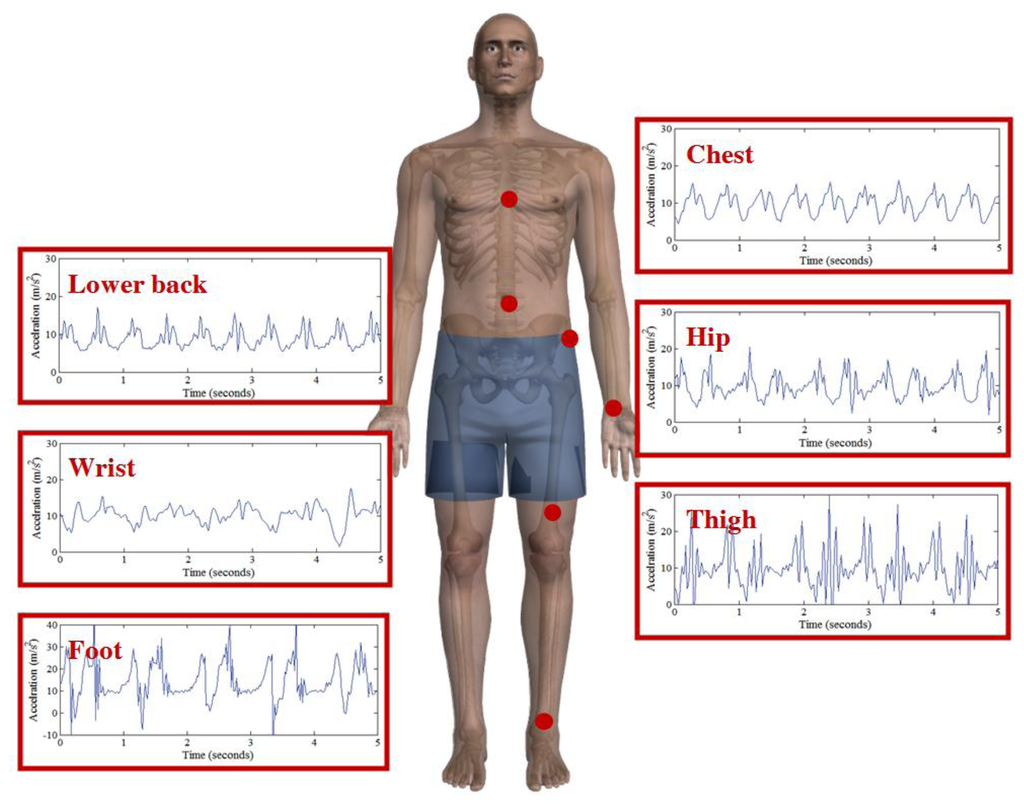
\includegraphics[width=0.8\textwidth]{Images/Chapter1/accelerometer-placement.png}
  \caption{تفاوت داده‌های تولیدی توسط حسگر شتاب‌سنج قرار گرفته در نقاط مختلف بدن}
  \label{fig:accelerometer-placement}
\end{figure}

علاوه بر مشکل تعمیم مدل بر روی داده‌های جدید، چالش برچسب‌گذاری داده‌ها نیز وجود دارد. چرا که برای برچسب‌گذاری داده‌های خام، نیاز به نیروی انسانی وجود دارد. برای مثال، مجموعه داده‌ی
\verb|ImageNet|
شامل 3.1 میلیون تصویر از 1000 کلاس مختلف می‌باشد که هر کدام از این تصاویر کاملا توسط نیروی انسانی برچسب خورده‌اند\cite{deng2009imagenet}.
طبیعتا برچسب‌گذاری این داده‌ها کاری بسیار طاقت‌فرسا و پرهزینه می‌باشد؛ اما برچسب‌گذاری داده‌های تصویری به مراتب ساده‌تر از برچسب‌گذاری داده‌های حسگرها می‌باشد. چرا که داده‌های تصویری برای افراد آشنا هستند و اشخاص می‌توانند با نگاه به تصاویر متوجه شوند که تصویر چه برچسبی را خواهد داشت. اما برای داده‌های حسگرها نمی‌توان صرفا از روی داده‌ی خام حسگر، فعالیت انجام شده‌ی مربوطه را به‌دست آورد. بنابراین برای برچسب‌گذاری داده‌ی حسگرها بایستی یک متخصص در تمام مدت آزمایش حرکات شخص مورد آزمایش را زیر نظر بگیرد و برچسب‌گذاری کند. این امر باعث می‌شود که برای تولید حجم زیادی داده‌ی برچسب‌دار برای مسئله‌ی شناسایی فعالیت انسان، زمان و هزینه‌ی بسیار زیادی صرف شود و علاوه بر آن داده‌ها در محیط آزمایشگاهی که با دنیای واقعی متفاوت هستند تولید شوند.

با توجه به دلایل ذکر شده، نیاز به روش‌هایی است که وابستگی مدل‌ها را به داده‌های برچسب‌خورده کاهش داده و در عین حال قدرت تعمیم آن‌ها را افزایش دهند. یکی از رویکردهای نوین برای رسیدن به این هدف، بهره‌گیری از یادگیری خودنظارتی\LTRfootnote{Self-Supervised Learning}
(که زیرمجموعه‌ای از یادگیری بدون نظارت\LTRfootnote{Unsupervised Learning} است)
می‌باشد. در این رویکرد، مدل با استفاده از ساختارهای درونی و الگوهای موجود در داده‌های بدون برچسب، پیش‌وظایفی را تحت عنوان
وظایف پوششی\LTRfootnote{Pretext tasks (Auxiliary tasks)}
اجرا می‌کند و مدل از آن‌ها برای یادگیری
بازنمایی‌های\LTRfootnote{Representation}
مفید بهره می‌برد. این پیش‌وظایف می‌تواند شامل مواردی مانند شناسایی چرخش\cite{gidaris2018unsupervised}،
روش‌های مبتنی بر ایجاد داده مانند تکمیل بخش‌های حذف‌شده از داده\cite{he2022masked}
و روش‌های مبتنی بر یادگیری تباینی\LTRfootnote{Contrastive Learning}\cite{chen2020simple,grill2020bootstrap,caron2020unsupervised}
باشند. همچنین در بسیاری از این روش‌ها، به‌منظور تقویت اثربخشی فرایند یادگیری، از تکنیک‌های
داده‌افزایی\LTRfootnote{Data Augmentation}
(مانند ایجاد نسخه‌های متغیر از یک نمونه‌ی داده با حفظ معنای کلی آن از طریق روش‌هایی مانند افزودن نویز و ایجاد برش بر روی داده‌ها) بهره گرفته می‌شود. با انجام این وظایف و حل این‌گونه مسائل، یک تابع هزینه نیز برای مدل تعریف می‌شود که مدل در طی فرایند کمینه کردن این تابع هزینه، بازنمایی‌های خوبی از داده یاد می‌گیرد که از وزن‌های تصادفی اولیه‌ی مدل عملکرد بسیار بهتری دارند.
سپس با استفاده از این بازنمایی‌ها می‌توان در مراحل بعدی برای حل وظایف دارای برچسب (مانند دسته‌بندی فعالیت‌ها) مدل را
تنظیم دقیق\LTRfootnote{Fine-tune}
کرد و عملکرد قابل قبولی را حتی با حجم کمی از داده‌های برچسب‌خورده به‌دست آورد\cite{gidaris2018unsupervised}.
استفاده از یادگیری خودنظارتی، نه تنها هزینه‌های مربوط به برچسب‌گذاری را به‌طور چشم‌گیری کاهش می‌دهد، بلکه با بهره‌گیری از حجم زیاد داده‌های بدون برچسب، قابلیت تعمیم مدل را نیز در مواجهه با داده‌هایی از توزیع‌های متفاوت افزایش می‌دهد. بدین صورت که می‌توان مدل را بر روی یک مجموعه داده‌ی بسیار بزرگ اما بدون برچسب پیش‌آموزش داد و سپس به‌وسیله‌ی
یادگیری انتقالی\LTRfootnote{Transfer Learning}،
بر روی مجموعه داده‌ی کوچک تنظیم دقیق انجام داد. تحقیقات نشان داده‌اند که پیش‌آموزش مدل به‌روش خودنظارتی و سپس تنظیم دقیق بر روی تنها بخش کوچکی از مجموعه داده‌ی مقصد
(یادگیری با نمونه‌ی اندک\LTRfootnote{Few-shot learning})،
عملکرد بهتری را نسبت به پیش‌آموزش به روش نظارت‌شده نشان می‌دهد\cite{chen2020big,yuan2024self}.
این ویژگی به‌ویژه در مسئله‌ی شناسایی فعالیت انسان که در آن تنوع بالایی در نحوه‌ی انجام فعالیت وجود دارد و همچنین کوچک‌ترین تغییراتی مانند وجود حیوان خانگی می‌تواند عملکرد مدل را مختل کند، از اهمیت بالایی برخوردار است. از این رو، استفاده از یادگیری خودنظارتی به عنوان یک راهکار جایگزین یا مکمل یادگیری نظارت‌شده گامی مؤثر در جهت ارتقای کارایی مدل‌ها در شرایط دنیای واقعی برداشته است.

\section{دستاوردهای پژوهش}

دستاوردهای کلی این پژوهش شامل موارد زیر می‌شوند:

\begin{itemize}
\item{استفاده از یک رویکرد یادگیری خودنظارتی تباینی بر مبنای خوشه‌بندی\LTRfootnote{Clustering}}
\item{استفاده از تبدیل موجک\LTRfootnote{Wavelet Transform} برای بهره‌گیری از مولفه‌های فرکانسی داده}
\item{بهبود روش‌های تولید داده‌ی افزوده برای تبدیل موجک}
\item{آزمایش و ارزیابی مدل ارائه شده در یادگیری انتقالی}
\end{itemize}

\section{ساختار مطالب}
در این پایان‌نامه،‌ فصل دوم به مرور پیشینه پژوهش و روش‌هایی که تاکنون در حوزه شناسایی فعالیت انسان، یادگیری خودنظارتی و کاربردهای یادگیری خودنظارتی در شناسایی فعالیت انسان ارائه شده‌اند اختصاص دارد. فصل سوم به معرفی مدل پیشنهادی این پژوهش پرداخته و ساختار مدل، الگوریتم‌های به‌کاررفته و نحوه استفاده از آن‌ها بررسی می‌گردد. در فصل چهارم، نتایج حاصل از آزمایش‌های انجام‌شده با استفاده از روش پیشنهادی در مقایسه با روش پایه ارائه می‌گردد و با تحلیل این نتایج، فصل خاتمه می‌یابد. در نهایت،‌ فصل پنجم به جمع‌بندی و نتیجه‌گیری و ارائه‌ی پیشنهاداتی برای کارهای آینده اختصاص دارد.

\chapter{ادبیات موضوع و کارهای پیشین}
\clearpage

در این فصل ابتدا به معرفی و بررسی مسئله‌ی شناسایی فعالیت‌های انسانی و پژوهش‌های انجام‌شده در این زمینه می‌پردازیم. در ادامه، به بررسی روش‌های یادگیری خودنظارتی، کاربرد آن‌ها در حوزه‌ی شناسایی فعالیت انسان، و پژوهش‌های مرتبط در این زمینه خواهیم پرداخت.

شناسایی فعالیت‌های انسانی یکی از مسائل مهم و پرکاربرد در حوزه‌های مختلف از جمله سلامت، خانه‌های هوشمند و پایش رفتار کاربران به‌شمار می‌رود. همان‌گونه که در فصل مقدمه نیز بیان شد، دو رویکرد کلی برای این مسئله وجود دارد: رویکرد مبتنی بر داده‌های تصویری و رویکرد مبتنی بر داده‌های حسگری. در این پژوهش، تمرکز اصلی بر استفاده از داده‌های حسگرها بوده و از این رو، روش‌های انتخاب‌شده نیز بر پایه‌ی این نوع داده‌ها طراحی و ارزیابی شده‌اند.

\section{شناسایی فعالیت انسان}

پیشرفت‌های مختلف در تکنولوژی، باعث شده‌اند که حسگرها با هزینه‌ی اندک تولید شوند و داده‌های تولید شده توسط آن‌ها با سرعت بالا پردازش شوند که در نتیجه‌ی آن کار با حسگرها در عمل ساده می‌شود و باعث تحقیقات متعددی در این حوزه شده است. علاوه بر آن، سیستم‌های هوشمند برای عملکرد مناسب نیازمند این هستند که فعالیت انجام شده توسط کاربر شناسایی شود تا سیستم بتواند به‌خوبی کار خود را انجام دهد. در ادامه چند مورد از کاربردهای کلی شناسایی فعالیت انسان در دنیای واقعی را شرح می‌دهیم:

\begin{itemize}
\item{سیستم‌های مراقبتی}

در بیشتر سیستم‌های سنتی مراقبتی، بیماران و افراد تحت مراقبت بایستی ارزیابی‌های دوره‌ای را انجام دهند که این موضوع علاوه بر زمان‌بر و هزینه‌بر بودن، دقیق نیست. چرا که این ارزیابی‌های دوره‌ای تنها وضعیت بیمار در لحظه را مورد سنجش قرار می‌دهند و ممکن است در یک زمانی بیمار مراجعه کند که علائم به خوبی دیده نشوند. به دلایل ذکر شده، سیستم‌های مراقبتی و پزشکی استقبال گسترده‌ای از روش‌های شناسایی فعالیت مبتنی بر انواع حسگرها کرده‌اند و تلاش‌ها در راستای هوشمندسازی هر چه بیشتر سیستم‌های مراقبتی ادامه دارد.

\item{دستیار زندگی در خانه‌های هوشمند}

از سیستم‌های شناسایی فعالیت می‌توان برای مراقبت از بیماران یا سالمندان در منزل و همچنین به‌عنوان دستیار زندگی بهره گرفت. برای مثال، سامانه‌ای هوشمند برای شناسایی فعالیت توسط الاقباری و همکاران طراحی شده که علاوه بر شناسایی فعالیت‌های روزمره، قابلیت تشخیص ناهنجاری‌ها\LTRfootnote{Anomaly} (مانند زمین خوردن فرد یا هر گونه اختلال در داده‌های حسگرها) و پیش‌بینی فعالیت بعدی (مثلاً پیش‌بینی ورود فرد به اتاق خواب و فعال‌سازی سیستم تهویه) را نیز دارد. چنین سیستمی می‌تواند به‌عنوان یک دستیار زندگی در خانه‌های هوشمند عملکرد مؤثری از خود نشان دهد \cite{alaghbari2022activities}.
‪
\end{itemize}

\subsection{تعریف مسئله}

برای مسئله‌ی شناسایی فعالیت انسان دو تعریف کلی می‌توان ارائه داد.

\noindent\textbf{تعریف اول:}


فرض کنید مجموعه‌ای به صورت \( S = \{s_0, s_1, \ldots, s_{k-1}\} \) در اختیار داریم که شامل \(k\) دنباله زمانی از اندازه‌گیری‌های مربوط به ویژگی‌های مختلف است. این داده‌ها در بازه‌ی زمانی \( I = [t_{\alpha}, t_{\omega}] \) ثبت شده‌اند. در مسئله‌ی تشخیص فعالیت، هدف این است که بازه‌ی زمانی \( I \) را به زیربازه‌هایی مانند \( I_0, I_1, \ldots, I_{r-1} \) تقسیم کنیم و برای هر زیربازه، برچسبی که بیانگر نوع فعالیت است اختصاص دهیم، به‌گونه‌ای که این برچسب‌گذاری با داده‌های \( S \) تطابق داشته باشد.

بر اساس این تعریف، زیربازه‌ها باید ناتهی و بدون هم‌پوشانی باشند و کل بازه زمانی \( I \) را پوشش دهند، یعنی \( I = \bigcup_{i=0}^{r-1} I_i \). بنابراین، فرض می‌شود که در هر لحظه تنها یک فعالیت در حال انجام است. هرچند این فرض در برخی شرایط دنیای واقعی ممکن است برقرار نباشد. برای نمونه، یک فرد ممکن است همزمان در حال آشپزی و مصرف دارو باشد. این مدل ساده، چارچوبی پایه برای طراحی سیستم‌های تشخیص فعالیت فراهم می‌کند.



\noindent\textbf{تعریف دوم:}


مجموعه‌ای از \( m \) پنجره زمانی به صورت \( W = \{w_0, w_1, \ldots, w_{m-1}\} \) را در نظر بگیرید، که هر پنجره‌ی \( w_i \) شامل توالی زمانی از مشاهدات سنسورها است. برای هر پنجره‌ی زمانی، داده‌های مربوطه با مجموعه‌ای مانند \( S_i = \{s_{i,0}, \ldots, s_{i,k-1}\} \) نمایش داده می‌شوند. همچنین فرض می‌کنیم مجموعه‌ای از برچسب‌ها تحت عنوان \( L = \{l_0, \ldots, l_{m-1}\} \) موجود است که هر عنصر آن نشان‌دهنده‌ی یک نوع فعالیت در بازه‌ی متناظر با یک پنجره‌ی زمانی می‌باشد.

در این صورت، می‌خواهیم تابعی تعریف کنیم به صورت \( f: S_i \mapsto L \) که بتواند با دریافت داده‌های هر پنجره \( S_i \)، مناسب‌ترین فعالیت از \( L \) را انتخاب کند. در واقع، این تابع تلاش می‌کند تشخیص دهد که در پنجره‌ی زمانی \( w_i \) کدام فعالیت غالب بوده است. اگرچه این شیوه به فرض غالب بودن یک فعالیت در هر پنجره استوار است، اما با در نظر گرفتن هم‌پوشانی جزئی یا نویز در داده‌ها، می‌تواند تخمینی مناسب از واقعیت ارائه دهد.

نکته‌ی مهم اینجاست که اگر دو پنجره زمانی پشت سر هم باشند، برچسب آن‌ها ممکن است مشابه باشد یا حتی در مرز پنجره‌ها، فعالیتی مشترک رخ دهد. با این حال، این روش باعث می‌شود مسئله به صورت برچسب‌گذاری دنباله‌ای از پنجره‌ها ساده‌سازی شده و امکان آموزش مدل‌های یادگیری ماشین فراهم گردد.

در مجموع، این مدل به ما اجازه می‌دهد با وجود پیچیدگی‌های ذاتی رفتارهای انسانی، از طریق تحلیل پنجره‌ای و نگاشت آن به برچسب‌ها، فرایند تشخیص فعالیت را قابل پیاده‌سازی و آموزش‌پذیر سازیم. این روش به‌ویژه در محیط‌های دارای داده‌های زیاد و پیوسته که فعالیت‌ها با یکدگیر همپوشانی دارند، بسیار کاربردی و موثر خواهد بود.

رویکرد کلی برای حل مسئله‌ی شناسایی فعالیت بدین صورت است که ابتدا نیاز به یک مجموعه داده‌ی
برچسب‌دار داریم. سپس با استفاده از این مجموعه داده‌ی برچسب‌دار، سعی می‌کنیم ویژگی‌هایی را استخراج کنیم و از آن‌ها برای آموزش مدل استفاده کنیم. بدین منظور چالش‌های متعددی بوجود می‌آیند که برای حل آن‌ها رویکردهای مختلفی توسط محققان ارائه شده‌اند که در ادامه به بررسی تعدادی از آن‌ها می‌پردازیم.

\subsection{سابقه پژوهش}

در زمینه‌ی شناسایی فعالیت‌های انسانی در کاربردهای مختلف کارهای متعددی انجام شده است. همرلا و همکاران\cite{hammerla2015pd}
حسگرهای پوشیدنی را به کفش‌های ۳۴ شخص مختلف دارای بیماری
پارکینسون\LTRfootnote{Parkinson's Disease}
متصل کردند. وظیفه‌ی این حسگرها اندازه‌گیری سرعت و شیوه راه رفتن افراد بود. سپس با استخراج ویژگی‌ها از روی مقادیر خام تولیدی توسط حسگرها و با استفاده از
ماشین بولتزمن محدود (\verb|RBM|\LTRfootnote{Restricted Boltzmann Machine}
اقدام به تشخیص بیماری پارکینسون در این افراد کردند.

یک کاربرد دیگر سیستم‌های شناسایی فعالیت که به آن اشاره کردیم، استفاده از آن برای دستیار زندگی و نظارت در خانه‌ی هوشمند می‌باشد. می‌توان از این سیستم‌ها برای مراقبت از بیماران مبتلا به
بیماری فراموشی\LTRfootnote{Alzheimer's Disease} و سالمندان استفاده کرد. محققان یک روش بر مبنای
مدل‌های پنهان مارکوف\LTRfootnote{Hidden Markov Models}
ارائه دادند که می‌تواند فعالیت‌های فرد ساکن خانه را شناسایی کند و موارد اضطراری و موارد مربوط به سلامت را گزارش دهد\cite{asghari2018activity}

به‌طور کلی، روش‌های مربوط به شناسایی فعالیت‌های انسانی به روش‌های مبتنی بر یادگیری ماشین و یادگیری عمیق روی آورده‌اند. مدل‌های یادگیری عمیق بسیاری برای برای شناسایی فعالیت پیشنهاد شده استو این مدل‌ها دقت خوبی را در آموزش با داده‌های برچسب‌دار به اندازه‌ی کافی
ارائه می‌کنند\cite{cook2013transfer}.
علاوه بر آن، روش‌های یادگیری عمیق در کاربردهای استخراج ویژگی در مسائل شناسایی فعالیت که داده‌های ورودی دارای ابعاد بالایی هستند به‌کار گرفته شده‌اند. روش‌های
داده محور\cite{chen2015deep}
و مدل محور چندوجهی\LTRfootnote{Multi-modal}\cite{ha2015multi}
دو روش کاربرد مدل عمیق در مسائل تشخیص فعالیت هستند.

یک راهکار که در گذشته به نتایج خوبی دست یافت، استفاده از روش‌های سنتی یادگیری ماشین است. روش
کا-نزدیک‌ترین همسایه (\verb|KNN|)
اگرچه یک روش ساده است،‌اما برای مثال توسط
فوستر و همکاران\cite{foerster1999detection}
برای شناسایی وضعیت بدن و جهت حرکت با استفاده از داده‌های حسگر به‌کار گرفته شد و نتایج خوبی از خود نشان داد. از دیگر روش‌های مورد استفاده نیز می‌توان
مدل‌های پنهان مارکوف\cite{asghari2018activity}،
جنگل تصادفی\LTRfootnote{Random Forest}\cite{attal2015physical}
و ماشین بردار پشتیبان (\verb|SVM|\LTRfootnote{Support Vector Machine})\cite{attal2015physical}
را نام برد که در دسته‌بدنی و شناسایی فعالیت‌های انسانی دارای عملکرد نسبتا خوبی هستند. مزیت این روش‌ها این است که بر خلاف روش‌های مبتنی بر یادگیری عمیق،‌ نیازمند تعداد داده‌ی بسیار زیادی نیستند و با تعداد داده‌ی کم می‌توانند نتایج خوبی را از خود نشان دهند\cite{chen2021deep}.
اما مشکلی که این روش‌ها دارند این است که نیازمند متخصص برای
استخراج ویژگی دستی\LTRfootnote{Handcrafted Features}
هستند و علاوه بر نیاز به متخصص، ویژگی‌های استخراج شده به اندازه‌ی کافی
انتزاعی\LTRfootnote{Abstract}
و پرکاربرد نیستند. بنابراین نمی‌توان به این روش‌ها در دنیای امروز که توزیع و ابعاد داده‌ها از پیچیدگی بالایی برخوردار هستند اکتفا کرد.

با پیشرفت شبکه‌های عصبی و فراهم شدن حجم زیاد داده‌ی برچسب‌دار و همه‌گیر شدن روش‌های مبتنی بر یادگیری عمیق، در سال‌های اخیر روش‌های شناسایی فعالیت نیز به استفاده از شبکه‌های عصبی روی آورده‌اند. چرا که داده‌ها در حوزه‌ی شناسایی فعالیت‌های انسانی عموما پیچیده و دارای ابعاد بالا و در برخی موارد چند وجهی هستند. محققان نشان دادند که با در نظر گرفتن داده‌ها بصورت چندوجهی و ترکیب داده‌های انواع مختلفی از حسگرها،‌به نتایج بهتری نسبت به حالتی که تنها از یک حسگر (مانند یک شتاب‌سنج) استفاده شده است می‌توان دست یافت\cite{guo2016wearable}.
علاوه بر آن، شبکه‌های عصبی عمیق به‌دلیل ساختار چند لایه و پیچیده‌ای که دارند، هر لایه می‌تواند ویژگی‌های مختلفی را از داده استخراج کند و نتیجتا امکان کار با داده‌های پیچیده‌تر را برایمان فراهم می‌کنند. برای استخراج ویژگی توسط شبکه‌های عصبی دیگر نیاز چندانی به مهندسی ویژگی به‌صورت پیچیده و کاملا دستی نخواهیم داشت و با ساختارهای خاصی می‌توان ویژگی‌ها را به‌صورت کاملا خودکار استخراج کرد. برای مثال، از شبکه‌های پیچشی یک بعدی و دو بعدی می‌توان در استخراج ویژگی‌ها و
وابستگی‌های مکانی\LTRfootnote{Spatial Dependencies}
(مثلا در تصاویر)
و همینطور از شبکه‌های بازگشتی\LTRfootnote{Recurrent Neural Network}
مانند حافظه‌ی کوتاه‌مدت بلند (\verb|LSTM|\LTRfootnote{Long Short-Term Memory})
یا واحد بازگشتی دروازه‌ای (\verb|GRU|\LTRfootnote{Gate Recurrent Unit})
در استخراج ویژگی‌ها و وابستگی‌های زمانی\LTRfootnote{Temporal Dependencies} استفاده کرد.

الاقباری و همکاران\cite{alaghbari2022activities}
در مقاله‌ی خود ۳ روش مختلف برای شناسایی فعالیت، شناسایی ناهنجاری و پیش‌بینی فعالیت ارائه دادند. آن‌ها برای هر فعالیت، یک مجموعه از \verb|R| ویژگی را تعریف می‌کنند که این ویژگی‌ها شامل موارد زیر می‌باشند:
\begin{enumerate}
    \item زمانی که برای انجام شدن فعالیت سپری شده است.
    \item تعداد حسگرهایی که در طول انجام فعالیت فعال بوده اند.
    \item تعداد دفعاتی که این فعالیت در طول روز انجام شده است.
    \item وضعیت (روشن/خاموش) تمام حسگرها
\end{enumerate}

با استفاده از تمامی این ویژگی‌ها مسئله به جای تحلیل سری به یک مسئله‌ی ساده‌تر تبدیل می‌شود که توسط
یک پرسپترون چند لایه (\verb|MLP|\LTRfootnote{Multi-Layer Perceptron})
عملیات دسته‌بندی و شناسایی فعالیت انجام می‌شود. در همین حین که شبکه‌ی پرسپترون چند لایه مشغول شناسایی فعالیت است، یک
شبکه‌ی خودکدگذار بیش‌کامل (\verb|OCDAE|\LTRfootnote{Over-Complete Deep Auto-Encoder})
وظیفه‌ی شناسایی ناهنجاری را دارد. بدین صورت که  همان \verb|R| ویژگی به این شبکه نیز داده می‌شوند و این شبکه سعی می‌کند که خروجی را از روی ورودی بازسازی کند. اگر که
خطای بازسازی\LTRfootnote{Reconstruction Error}
کم بود، بدین معناست که فعالیت مربوطه مانند یکی از فعالیت‌هایی است که شبکه قبلا بر روی آن آموزش دیده و در غیر اینصورت یک ناهنجاری شناسایی می‌شود.
\begin{figure}[htbp]
  \centering
  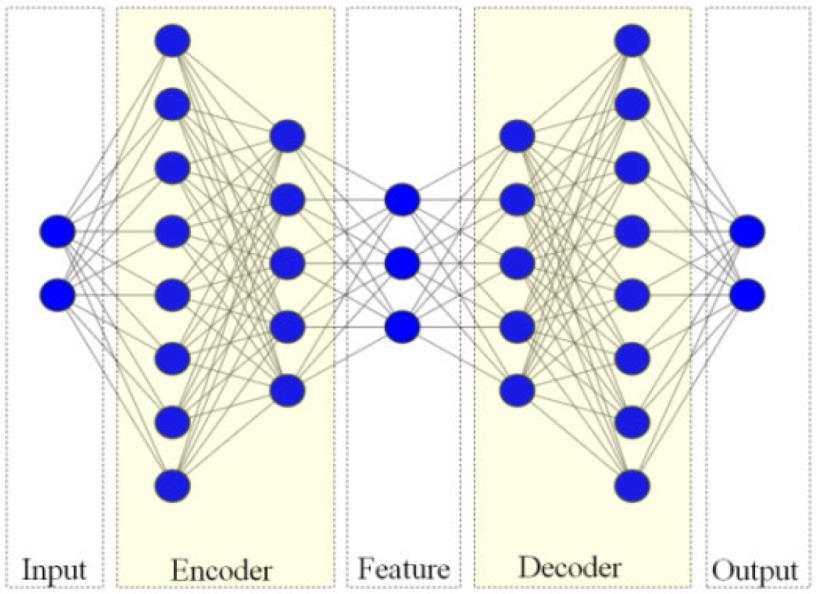
\includegraphics[width=0.8\textwidth]{Images/Chapter2/ocd-ae.png}
  \caption{ساختار خودکدگذار عمیق بیش‌کامل}
  \label{fig:ocd-ae}
\end{figure}
در عین حال که این ۲ شبکه کار می‌کنند، اگر که ناهنجاری شناسایی نشود خروجی شبکه‌ی شناسایی کننده‌ی فعالیت به‌عنوان فعالیت فعلی در نظر گرفته می‌شود و سپس توسط یک شبکه‌ی حافظه‌ی کوتاه‌مدت بلند، فعالیت بعدی پیش‌بینی می‌شود. شکل کلی ساختار پیاده شده در این مقاله به فرم شکل \ref{fig:alaghbari-framework} می‌باشد.
\begin{figure}[htbp]
  \centering
  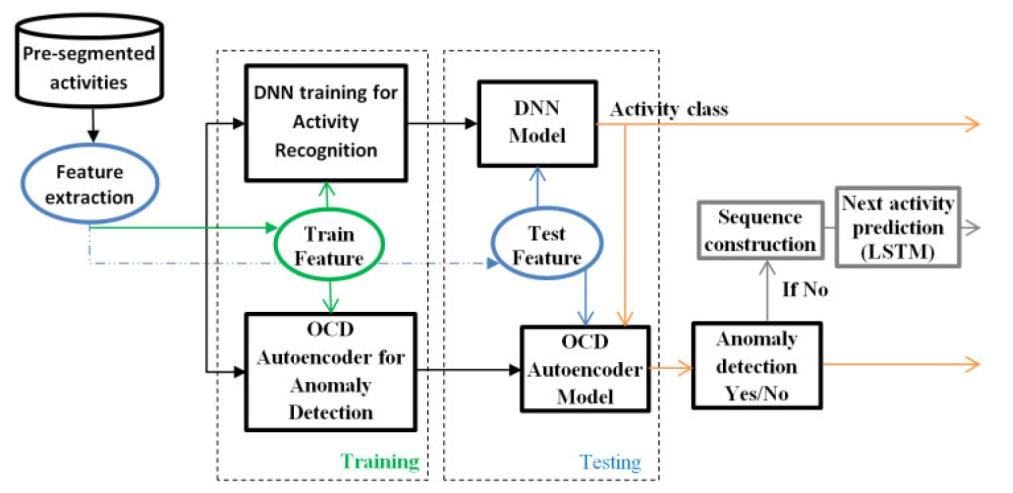
\includegraphics[width=0.8\textwidth]{Images/Chapter2/alaghbari-framework.png}
  \caption{معماری سیستم تشخیص فعالیت، ناهنجاری و پیش‌بینی فعالیت بعدی}
  \label{fig:alaghbari-framework}
\end{figure}

گائو و همکاران\cite{gao2021danhar}
یک روش بر مبنای سازوکار توجه\LTRfootnote{Attention Mechanism}
و توجه دوگانه\LTRfootnote{Dual Attention}
ارائه دادند. سازوکار توجه به شبکه‌ی عصبی این امکان را می‌دهد که به مرور یاد بگیرد که به کدام بخش‌های داده توجه بیشتری نشان دهد. برای مثال سازوکار توجه در داده‌ی تصویری به شبکه این امکان را می‌دهد که به بخش‌های مهم‌تر تصویر اهمیت بیشتری نشان بدهد و شبکه بتواند ویژگی‌های مهم‌تری را استخراج کند. توجه دوگانه بدین صورت عمل می‌کند که سازوکار توجه به‌طور همزمان برای دو نوع داده (مثلا تصویر و داده‌ی دنباله‌ای مانند متن) به‌کار گرفته شود.

بدین ترتیب گائو و همکاران از توجه دوگانه برای مسئله‌ی شناسایی فعالیت انسان استفاده کردند. روش ارائه شده چند بخش اصلی دارد:
\begin{enumerate}
    \item \textbf{ورودی داده‌های سنسورها:}
    سیگنال‌های چند-کاناله‌ی حسگرها (مانند شتاب‌سنج و ژیروسکوپ) به عنوان ورودی به مدل داده می‌شوند.

    \item \textbf{استخراج ویژگی با شبکه‌های پیچشی:}
    با عبور داده‌ها از چندین لایه شبکه‌ی پیچشی، ویژگی‌های سطح پایین و میانی استخراج می‌شوند.

    \item \textbf{ماژول توجه دوگانه:}
    پس از استخراج ویژگی، ویژگی‌های به‌دست‌آمده به ماژول توجه دوگانه داده می‌شوند. این ماژول شامل:
    \begin{itemize}
        \item \textbf{توجه کانالی\LTRfootnote{Channel Attention}:} محاسبه‌ی وزن برای هر کانال از ویژگی‌ها به‌منظور تعیین اهمیت سنسورها و ویژگی‌های مختلف و تقویت ویژگی‌های مهم.
        \item \textbf{توجه زمانی\LTRfootnote{Temporal Attention}:} محاسبه‌ی وزن برای هر گام زمانی به‌منظور تمرکز روی بازه‌های زمانی مهم در طول فعالیت.
    \end{itemize}
    ویژگی‌های خروجی از این دو توجه به‌ترتیب روی ویژگی‌ها ضرب می‌شوند و بازنمایی غنی‌شده‌ای از داده تولید می‌شود.

    \item \textbf{تکرار فرایند استخراج ویژگی و توجه:}
    فرایند استخراج ویژگی و ماژول توجه دوگانه یک بار دیگر تکرار می‌شود تا ویژگی‌های سطح بالاتری استخراج شوند.

    \item \textbf{لایه‌های دسته‌بندی:}
    در نهایت، ویژگی‌های استخراج و وزن‌دهی شده به لایه‌های تماما متصل\LTRfootnote{Fully Connected} داده می‌شوند تا فعالیت مربوطه پیش‌بینی شود.
\end{enumerate}
\begin{figure}[htbp]
  \centering
  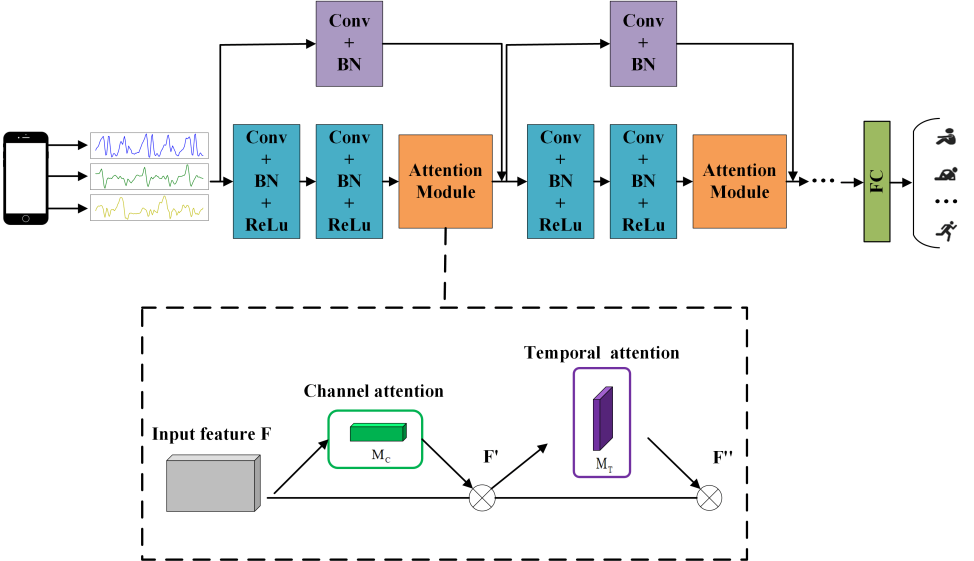
\includegraphics[width=0.8\textwidth]{Images/Chapter2/danhar.png}
  \caption{معماری سیستم توجه دوگانه بر روی داده‌های حسگر}
  \label{fig:danhar}
\end{figure}

وانگ و همکاران\cite{wang2020wearable} یک روش مبتنی بر ترکیب شبکه پیچشی و شبکه حافظه کوتاه‌مدت بلند ارائه کردند که به دقت بالایی دست یافت. در این روش، از داده‌های مربوط به سری زمانی دو حسگر ۳ کاناله شتاب‌سنج و ژیروسکوپ ابتدا
پنجره‌های لغزان\LTRfootnote{Sliding Windows}
دارای همپوشانی استخراج می‌شوند و سپس داده‌های هر ۶ کانال حسگرها به صورت یک تصویر در کنار هم قرار می‌گیرند. بدین صورت یک تصویر به طول پنجره‌ی لغزان و عرض ۶ خواهیم داشت. سپس بر روی این شبه تصاویر لایه‌های پیچشی اعمال می‌شوند و آرایه‌ای از این شبه تصاویر توسط لایه‌های پیچشی پردازش می‌شوند تا ویژگی‌های هر پنجره که با دیگر پنجره‌ها همپوشانی دارد استخراج شوند. سپس این دنباله ویژگی‌های استخراج شده به یک شبکه حافظه کوتاه‌مدت بلند داده می‌شود که خروجی آن مجموعه‌ای از بردارها است که شامل وابستگی‌های زمانی و توالی فعالیت‌ها می‌باشد. این بردارها به لایه‌ی تماما متصل داده می‌شوند تا ویژگی‌های کلی فعالیت با یکدیگر
ترکیب\LTRfootnote{Fusion}
شده و به‌صورت یکپارچه استخراج شوند. ضمنا جهت پایداری بیشتر یادگیری و دستیابی به دقت بالاتر، نویسندگان مقاله از
نرمال‌سازی دسته‌ای\LTRfootnote{Batch Normalization}
استفاده کردند.

\section{یادگیری خودنظارتی}

همانطور که در بخش قبل بررسی کردیم، شبکه‌های عصبی عمیق در مواردی که داده‌ها از پیچیدگی بالایی برخوردار هستند و ابعاد داده‌های ورودی بالا هستند، شدیدا از روش‌های سنتی یادگیری ماشین عملکرد بهتر و قدرتمندتری دارند و نتایج دقیق‌تری را از خود نشان می‌دهند. در واقع می‌توان گفت که در کاربردهای پیشرفته‌ی دنیای امروز استفاده از یادگیری عمیق به روش‌های یادگیری ماشین سنتی در اکثر مواقع ترجیح داده می‌شوند. اما چالش اصلی روش‌های مبتنی بر یادگیری عمیق نیاز شدید این روش‌ها به حجم زیادی داده برچسب‌گذاری شده می‌باشد. آنچه که در دنیای امروز شدیدا فراوان و در دسترس است، انواع داده بدون برچسب می‌باشد و به‌طور کلی جمع‌آوری داده‌ی خام کاری نسبتا ساده و کم‌هزینه می‌باشد. اما برچسب‌گذاری داده‌ها کاری شدیدا پرهزینه و زمان‌بر می‌باشد. در واقع یکی از اصلی‌ترین
گلوگاه‌های\LTRfootnote{Bottleneck}
آموزش شبکه‌های عصبی عمیق، جمع‌آوری داده‌ی آموزشی دارای برچسب می‌باشد.

علاوه بر هزینه‌ها و چالش‌های ناشی از برچسب‌گذاری داده‌ها، یادگیری تحت نظارت دارای مشکلاتی مانند 
خطای تعمیم\LTRfootnote{Generalization Error}،
همبستگی‌های کاذب\LTRfootnote{Spurious Correlations}
و برچسب‌گذاری‌های غلط غیر عمدی و یا عمدی ناشی از حملات خصمانه\LTRfootnote{Adversarial Attacks}
می‌باشد\cite{liu2021self}.

با توجه به تمامی چالش‌های ذکر شده، ضروری است که به سراغ روش‌هایی برویم که وابستگی ما را به مجموعه داده‌های برچسب‌دار کاهش دهند. هدف اصلی، دستیابی به قابلیت اجرای مانند دسته‌بندی تنها با اتکا به حجم به مراتب کمتری از داده‌های برچسب‌خورده است.

برای تحقق این هدف، رویکردهایی مانند یادگیری خودنظارتی بسیار کارآمد هستند. روش‌های مبتنی بر یادگیری خودنظارتی به ما اجازه می‌دهند تا از ظرفیت عظیم داده‌های بدون برجسب که به وفور یافت می‌وشند و دسترسی به آن‌ها کم‌هزینه‌تر است بهره ببریم. در این شیوه، مدل ابتدا با استفاده از داده‌های خام و بدون برچسب، یک درک پایه‌ای و غنی از ساختار و ویژگی‌های داده‌ها پیدا می‌کند. سپس این مدل پیش‌آموخته را می‌توان با مقدار بسیار اندکی از داده‌های برچسب‌دار برای عملیات نهایی مورد نظر تنظیم دقیق کنیم. این رویکرد نه تنها باعث صرفه‌جویی چشمگیری در هزینه و زمان برچسب‌زنی می‌شود، بلکه به مدل اجازه می‌دهد تا با یادگیری از گستره وسیع‌تری از داده‌ها، به تعمیم‌پذیری و عملکرد بهتری دست یابد.

\begin{figure}[htbp]
  \centering
  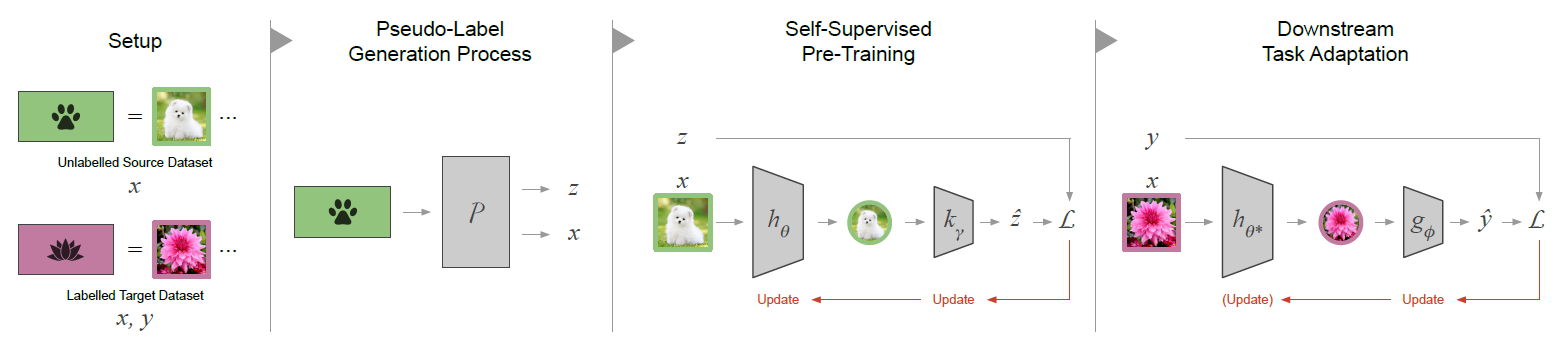
\includegraphics[width=1.0\textwidth]{Images/Chapter2/selfsupervised-overview.png}
  \caption{ساختار کلی سیستم‌های یادگیری خودنظارتی}
  \label{fig:selfsupervised-overview}
\end{figure}

\subsection{تعریف یادگیری خودنظارتی}

پیش از ارائه‌ی یک تعریف برای یادگیری خودنظارتی، برای درک بهتر مفاهیم بکار گرفته شده در این پایان‌نامه به بیان برخی از اصطلاحات که در این حوزه رایج هستند می‌پردازیم:

\begin{itemize}
    \item \textbf{شبه برچسب:}
    در حقیقت، شبه‌برچسب‌ها برچسب‌هایی هستند که معمولا به‌صورت خودکار و بر اساس ویژگی‌های داده‌ها در فاز اول آموزش (پیش‌آموزش) برای هر داده تولید می‌شوند. برای مثال در وظیفه‌ی پوششی شناسایی میزان چرخش تصویر، شبه برچسب مربوطه میزان چرخش اعمال شده به این تصویر می‌باشد.
    \item \textbf{وظیفه پوششی:}
    وظیفه پوششی در واقع وظیفه‌ای است که برای اجرای فاز پیش‌آموزش خودنظارتی طراحی شده و هدف آن یادگیری ویژگی‌های سطح بالا از روی داده‌های خام با کمک شبه‌برچسب‌ها می‌باشد. این وظیفه در حقیقت معماری شبکه و نحوه یادگیری ویژگی‌ها در فاز پیش‌آموزش خودنظارتی را تعیین می‌کند.
    \item \textbf{وظیفه پایین‌دستی\LTRfootnote{Downstream Task}:}
    وظیفه پایین‌دستی در واقع همان وظیفه اصلی است که پس از فاز پیش‌آموزش خودنظارتی انجام می‌شود که به‌طور کلی به دو منظور انجام می‌شود. هدف اول، ارزیابی کیفیت ویژگی‌های استخراج شده توسط شبکه‌ی پیش‌آموزش دیده و هدف دوم، آموزش نهایی مدل برای هدف اصلی (مثلا شناسایی فعالیت انسان یا دسته‌بندی تصاویر) می‌باشد. در واقع وظیفه‌ی پایین‌دستی شامل وظایف مستقل از پیش‌آموزش خودنظارتی است که مدل پیش‌آموزش دیده شده را به‌صورت کاربردی مورد ارزیابی قرار می‌دهد و آن را برای کاربردهای دنیای واقعی آماده می‌کند.
\end{itemize}

یادگیری خودنظارتی، یک رویکرد یادگیری ماشین است که در آن مدل بدون استفاده از برچسب‌های داده‌ها و مجموعه داده‌ی برچسب‌دار، از داده‌های بدون برچسب برای یادگیری بازنمایی‌های مفید استفاده می‌کند. در این روش، با ایجاد شبه برچسب‌ها از داده‌های ورودی بدون برچسب (مثلا حذف بخشی از داده و تلاش برای بازسازی آن) یک وظیفه پوششی تعریف می‌کنیم تا مدل بتواند ساختارها و الگوهای درونی داده را یاد بگیرد. سپس این بازنمایی‌های آموخته شده می‌توانند برای حل وظایف پایین‌دستی اصلی مانند دسته‌بندی مورد استفاده قرار بگیرند. نکته‌ی حائز اهمیت در اینجا این است که با تعداد بسیار کمتری داده‌ی برچسب‌دار می‌توان آموزش مدل را انجام داد و به قدرت تعمیم بالایی دست یافت.

\begin{figure}[htbp]
  \centering
  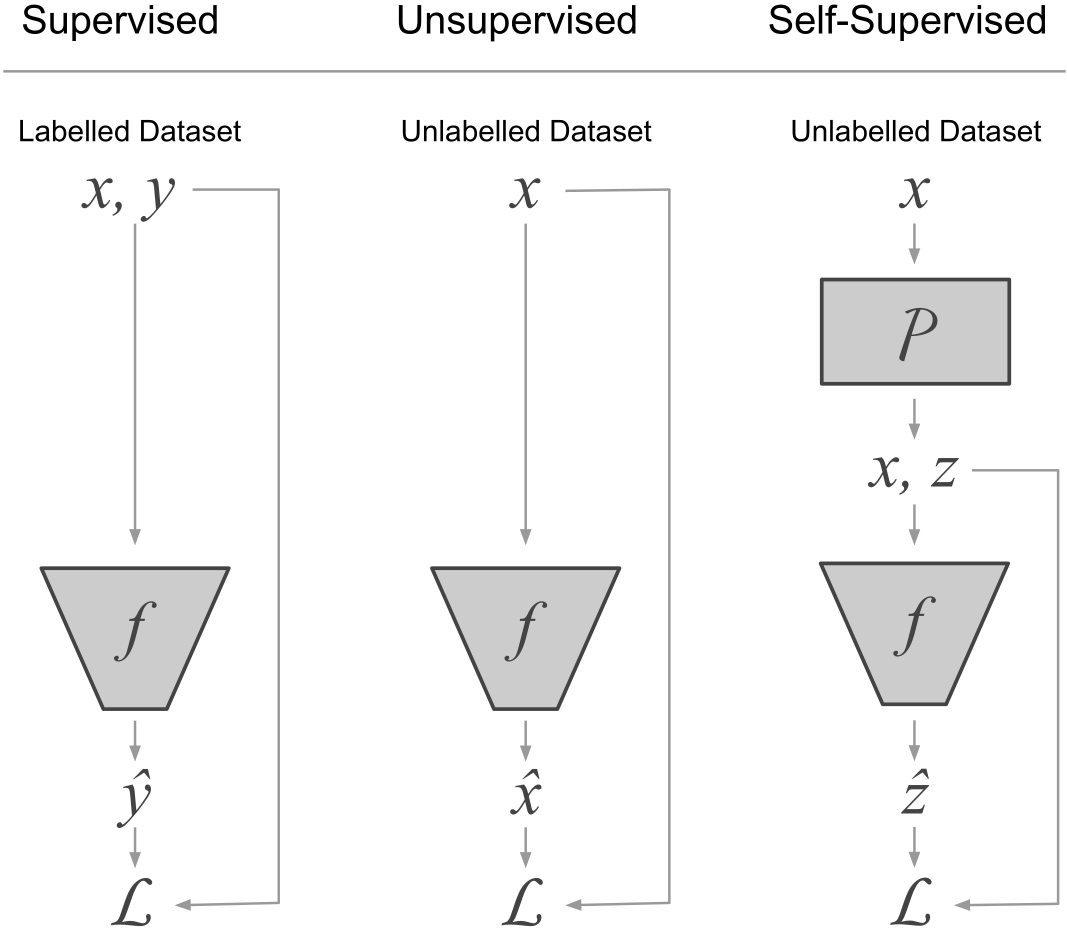
\includegraphics[width=0.7\textwidth]{Images/Chapter2/self-vs-unsupervised.png}
  \caption{ساختار کلی سیستم‌های یادگیری خودنظارتی}
  \label{fig:self-vs-unsupervised}
\end{figure}

همانطور که در شکل \ref{fig:self-vs-unsupervised}
دیده می‌شود، یادگیری خودنظارتی در اصل نوعی از یادگیری بدون نظارت است\cite{ericsson2022self}.
یادگیری بدون نظارت شامل الگوریتم‌هایی مانند انواع
الگوریتم‌های خوشه‌بندی\LTRfootnote{Clustering}،
شبکه‌ی مولد تخاصمی (\verb|GAN|\LTRfootnote{Generative Adversarial Network})
و خودکدگذار متغیر (\verb|VAE|\LTRfootnote{Variation Auto-Encoder})
می‌باشد. یادگیری خودنظارتی نیز در این موضوع که مجموعه داده بدون برچسب می‌باشد با یادگیری بدون نظارت مشترک است. اما معماری کلی و
بهینه‌سازی\LTRfootnote{Optimization}
مدل‌های یادگیری خودنظارتی به روش‌های یادگیری نظارت‌شده نزدیک‌تر است. چرا که سیگنال نظارت را توسط شبه برچسب‌ها و وظایف پوششی اعمال می‌کنیم و با شبه برچسب‌ها می‌توان دقیقا مانند یک برچسب واقعی رفتار کنیم و عمل دسته‌بندی و بهینه‌سازی مدل را با محاسبه‌ی خطای دسته‌بندی انجام دهیم.

\subsubsection{فرمول‌بندی یادگیری خودنظارتی}

در یادگیری خودنظارتی، برخلاف یادگیری با نظارت که به داده‌های جفت‌شده‌ی $X_i$ و $Y_i$ نیاز دارد (که $Y_i$ توسط نیروی انسانی برچسب‌گذاری می‌شود)، از برچسب‌هایی استفاده می‌شود که به صورت خودکار و بدون نیاز به مداخله‌ی انسانی تولید می‌شوند. این برچسب‌های خودکار یا شبه‌برچسب‌ها ($P_i$) مستقیماً از ویژگی‌های درونی داده‌ها (مانند تصاویر یا داده‌های سری‌زمانی) و با استفاده از قواعد و طراحی الگوریتمی مناسب استخراج می‌گردند. بنابراین با داشتن $N$ نمونه داده‌ی آموزشی، تابع هزینه در یادگیری با نظارت طبق رابطه‌ی زیر محاسبه می‌شود \cite{jing2020self}:

\begin{equation}
\label{eq:1-2}
loss(D) = \min_{\theta} \frac{1}{N} \sum_{i=1}^{N} loss(f_θ(X_i), Y_i)
\end{equation}

اما در فاز نخست یادگیری خودنظارتی که با هدف یادگیری بازنمایی‌های غنی از داده‌ها و استخراج ویژگی‌های باکیفیت بدون نیاز به برچسب انسانی انجام می‌شود، تابع هزینه‌ی رابطه‌ی \ref{eq:1-2} به شکل زیر تغییر پیدا می‌کند:

\begin{equation}
\label{eq:2-2}
loss(D) = \min_{\theta} \frac{1}{N} \sum_{i=1}^{N} loss(f_θ(X_i), P_i)
\end{equation}

در این معادلات، $f_θ(X_i)$ به این معنا است که ابتدا خروجی شبکه برای $X_i$ محاسبه می‌گردد و سپس مقدار آن با برچسب‌ها یا شبه برچسب‌ها مقایسه می‌شود و هزینه محاسبه می‌گردد. این فرایند باعث می‌شود که شبکه به‌تدریج پارامترهای خود را به گونه‌ای تنظیم نماید که خروجی‌های تولید شده بیشترین تطابق را با برچسب‌های موجود داشته باشند و در نتیجه مدل قادر به یادگیری الگوهای موثر و معنادار از داده‌های ورودی گردد.

پس از پایان این مرحله، مدل آموزش‌دیده در فاز پیش‌آموزش خودنظارتی آماده می‌شود تا در مرحله‌ی بعدی، یعنی آموزش با نظارت در وظایف پایین‌دستی مورد استفاده قرار گیرد. در این مرحله، از بازنمایی‌های یادگرفته‌شده توسط مدل برای بهبود کارایی و کاهش نیاز به داده‌های برچسب‌خورده‌ی فراوان استفاده می‌شود و فرایند یادگیری انتقالی به اجرا درمی‌آید.

\subsection{سابقه پژوهش}

به‌طور کلی کارهای انجام شده در حوزه‌ی یادگیری خودنظارتی را می‌توان بر حسب ماهیت وظیفه‌ی پوششی مورد استفاده به چند دسته‌ی کلی تقسیم‌بندی کرد:

\begin{enumerate}

\item \textbf{روش‌های زمینه‌محور\LTRfootnote{Context-based}:} \
در این دسته از روش‌ها، هدف مدل، یادگیری روابط میان اجزای مختلف داده با استفاده از زمینه‌ی محلی یا سراسری آن است. این روش‌ها معمولاً بر پایه‌ی روش‌هایی مانند پیش‌بینی موقعیت نسبی بخش‌های داده، ترتیب وقوع رویدادها، یا ویژگی‌های ساختاری مانند شناسایی جهت چرخش یا ترتیب قطعات بنا می‌شوند. از آنجا که این وظایف معمولاً نیاز به بازسازی کامل داده ندارند و تنها از اطلاعات ضمنی در خود داده استفاده می‌کنند، پیاده‌سازی نسبتاً ساده‌تری دارند و در حوزه‌هایی نظیر پردازش تصویر و تحلیل سیگنال کاربرد گسترده‌ای یافته‌اند.

\item \textbf{روش‌های بازسازی‌محور\LTRfootnote{Reconstruction-based}:} \
در این روش‌ها، شبکه تلاش می‌کند تا ورودی ناقص، دارای نویز یا کدگذاری‌شده را بازسازی کند. این دسته شامل خانواده‌ی گسترده‌ای از روش‌های مولد\LTRfootnote{Generative}
نیز می‌شود، از جمله خوکدگذارها، حذف نویز، رنگی‌سازی تصاویر، و پر کردن بخش‌های حذف‌شده از داده. تمرکز اصلی این رویکردها بر حفظ اطلاعات کامل از ورودی در بازنمایی‌های آموخته‌شده است. چنین بازنمایی‌هایی معمولاً ظرفیت بالایی برای انتقال به وظایف پایین‌دستی مانند طبقه‌بندی یا تشخیص دارند.

\item \textbf{روش‌های برچسب معنایی‌محور\LTRfootnote{Semantic Label-based}:} \
در این رویکردها، هدف از وظیفه‌ی پوششی، پیش‌بینی برچسب‌هایی است که به‌صورت خودکار و بدون دخالت انسان از داده استخراج شده‌اند، اما نمایانگر مفاهیم سطح بالای معنایی هستند. برای نمونه، دسته‌بندی داده‌ها بر اساس خوشه‌بندی بازنمایی‌های اولیه یا پیش‌بینی ویژگی‌هایی که نمایانگر ساختار مفهومی داده هستند. در واقع، این روش‌ها سعی می‌کنند با اجرای الگوریتم‌هایی، یک یا چند برچسب برای داده‌ها استخراج کنند و یادگیری را با استفاده از این برچسب‌ها انجام می‌دهیم. به همین دلیل، معمولاً از مکانیزم‌هایی مانند خوشه‌بندی، خودتقطیر\LTRfootnote{Self-distillation}،
یا یادگیری مبتنی بر نماینده‌ها بهره می‌برند. در این پایان‌نامه با جزئیات به آن نمی‌پردازیم اما نمونه‌ای از کاربرد این روش را می‌توان در مقاله‌ی ارائه شده توسط دتون و همکاران\cite{detone2018superpoint}
مشاهده نمود.

\item \textbf{روش‌های تباینی:} \
این دسته از روش‌ها بر اساس اصل نزدیک‌سازی نمونه‌های مشابه و دورسازی نمونه‌های ناسازگار از یکدیگر عمل می‌کنند. در این رویکرد، نمونه‌های مثبت (مانند دو نمایش\LTRfootnote{View}
مختلف از یک داده) باید در فضای بازنمایی به یکدیگر نزدیک شوند و نمونه‌های منفی (مانند دو نمایش مختلف از دو داده‌ی مختلف) از هم فاصله بگیرند. این مکانیزم باعث می‌شود که مدل، بازنمایی‌هایی مقاوم نسبت به تغییرات بی‌اهمیت یاد بگیرد. روش‌های تباینی نقش مهمی در موفقیت یادگیری خودنظارتی مدرن داشته‌اند و پایه‌گذار بسیاری از مدل‌های پیشرفته در حوزه‌های تصویر، ویدیو و سیگنال هستند.

\end{enumerate}

در ادامه، به بررسی دقیق‌تر هریک از دسته‌های یادگیری خودنظارتی معرفی شده در بالا پرداخته و نمونه‌هایی از روش‌های برجسته در هر دسته معرفی می‌شوند.

\subsubsection{روش‌های زمینه‌محور}

در روش‌های زمینه‌محور، ایده‌ی اصلی استفاده از اطلاعات زمینه‌ای موجود در خود داده برای تعریف یک وظیفه‌ی یادگیری است. این وظایف معمولا بر پایه‌ی روابط مکانی، زمانی یا ساختاری میان اجزای مختلف یک نمونه شکل می‌گیرند. چنین روش‌هایی با بهره‌گیری از ساختار درونی داده، سعی در استخراج بازنمایی‌هایی دارند که بتوانند موقعیت، ترتیب، یا سایر روابط میان اجزا را درک کنند. این دسته از روش‌ها به‌ویژه در حوزه‌های بینایی ماشین و تحلیل سیگنال، نقطه‌ی آغاز پژوهش‌های جدی در یادگیری خودنظارتی بوده‌اند و هنوز هم کاربرد گسترده‌ای دارند.\newline\newline

\noindent\textbf{وظیفه‌ی پوششی پیش‌بینی چرخش:}

یکی از وظایف پوششی مشهور در حوزه‌ی یادگیری خودنظارتی، پیش‌بینی میزان چرخش اعمال‌شده بر تصویر است. این وظیفه که نخستین بار در مقاله‌ی \lr{RotNet} \cite{gidaris2018unsupervised} معرفی شد، بر این فرض استوار است که یک شبکه‌ی عصبی تنها در صورتی قادر به تشخیص زاویه‌ی چرخش یک تصویر خواهد بود که بتواند به درک عمیقی از ساختار درونی و مفاهیم معنایی موجود در تصویر دست یابد. از این رو، پیش‌بینی چرخش به‌عنوان یک وظیفه‌ی ساده و مشخص، در عمل منجر به یادگیری بازنمایی‌هایی می‌شود که برای بسیاری از وظایف پایین‌دستی نیز قابل انتقال هستند.

در پیاده‌سازی اولیه‌ی این ایده، تصویر ورودی به‌صورت تصادفی یکی از چهار چرخش صفر، ۹۰، ۱۸۰ یا ۲۷۰ درجه را دریافت می‌کند. مدل باید زاویه‌ی صحیح را از میان چهار گزینه تشخیص دهد. برای این منظور، ساختار مدل از چندین لایه‌ی پیچشی  برای استخراج ویژگی استفاده می‌کند و در نهایت به یک لایه‌ی کاملاً متصل با چهار نورون خروجی منتهی می‌شود که هر نورون نمایانگر یکی از کلاس‌های زاویه‌ی چرخش است. این ساختار در شکل \ref{fig:rotnet} نمایش داده شده است.

\begin{figure}[htbp]
\centering
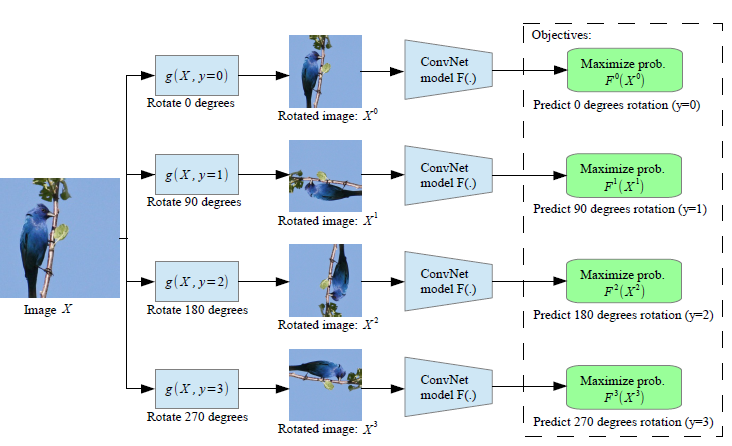
\includegraphics[width=0.8\textwidth]{Images/Chapter2/rotnet.png}
\caption{ساختار کلی شبکه‌ی پیش‌بینی چرخش}
\label{fig:rotnet}
\end{figure}

برتری اصلی این روش در آن است که بدون استفاده از هیچ‌گونه برچسب دستی، مدل را وادار می‌کند تا ساختار اشیاء، موقعیت اجزای تصویر و ویژگی‌های کلان معنایی را در بازنمایی‌های درونی خود بیاموزد. این بازنمایی‌ها در مراحل بعدی می‌توانند برای وظایفی نظیر طبقه‌بندی تصویر یا شناسایی اشیاء مورد استفاده قرار گیرند.

\begin{table}[htbp]
\centering
\caption{مقایسه‌ی عملکرد روش پیش‌بینی چرخش }
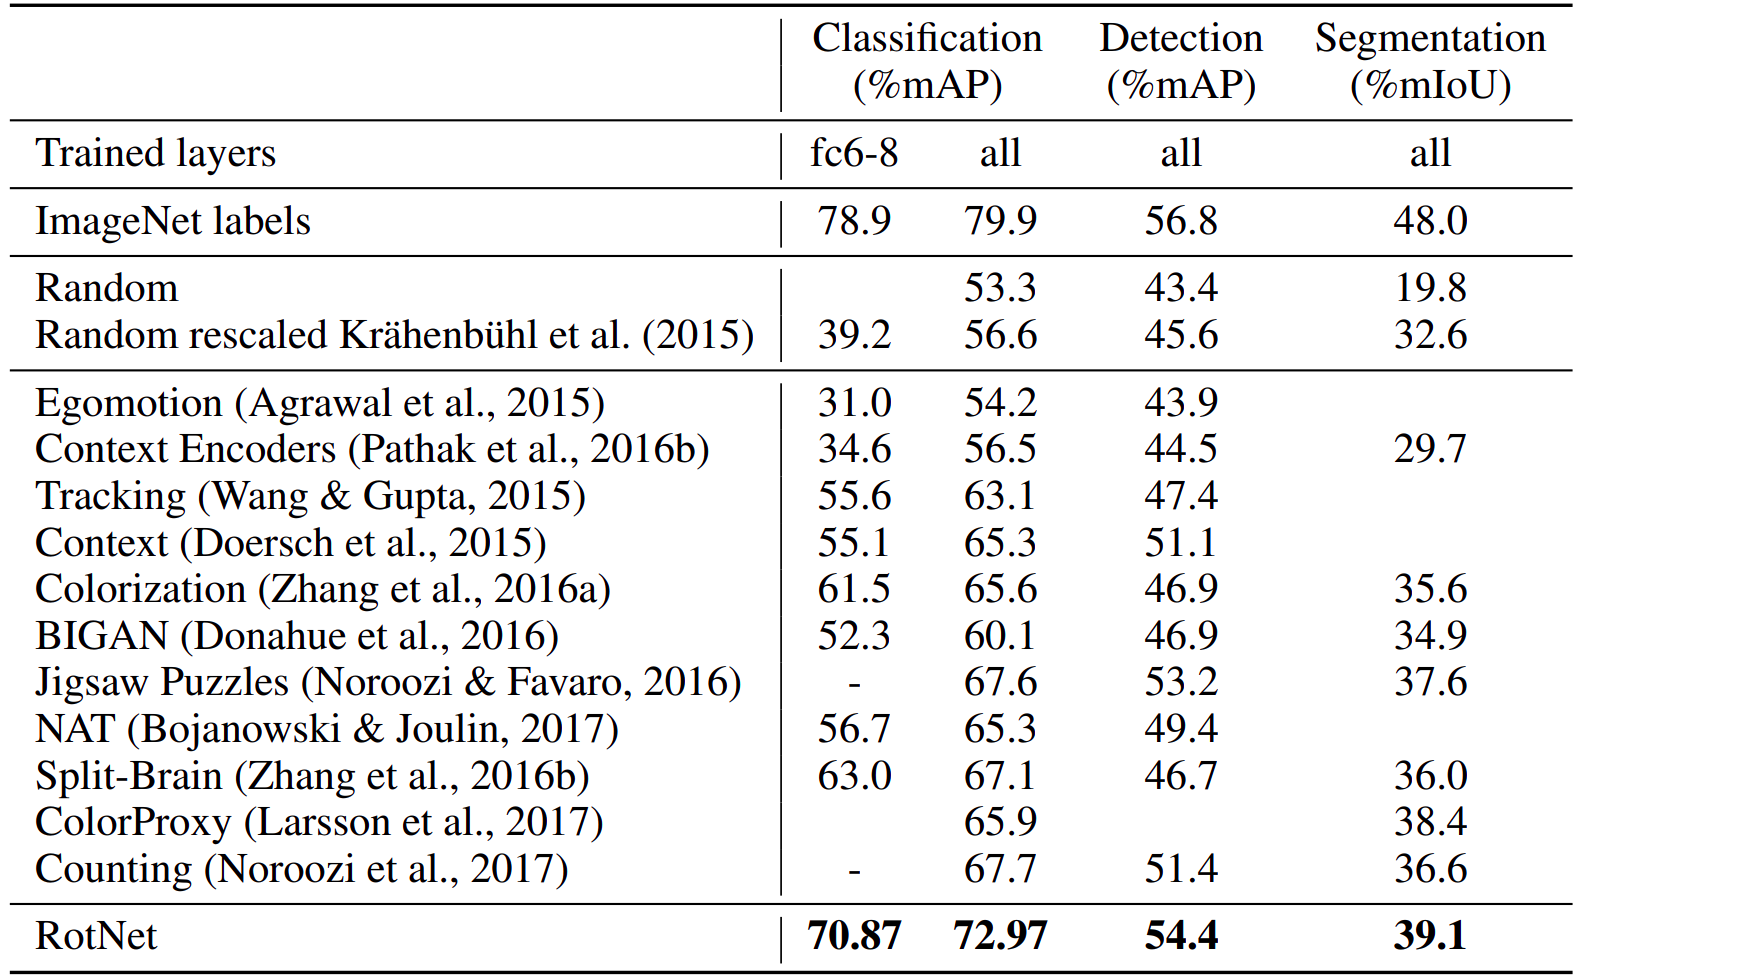
\includegraphics[width=0.8\textwidth]{Images/Chapter2/rotnet-results.png}
\label{tab:rotnet-results}
\end{table}

همان‌گونه که در جدول
\ref{tab:rotnet-results}
دیده می‌شود، عملکرد مدل پیش‌آموزش‌دیده با استفاده از وظیفه‌ی پوششی پیش‌بینی چرخش و سپس تنظیم دقیق برای انجام وظیفه‌ی پایین‌دستی اصلی، نه‌تنها از سایر روش‌های خودنظارتی و بدون نظارت موجود در زمان خود پیشی گرفته، بلکه عملکردی نزدیک به مدل‌های نظارت‌شده نیز از خود نشان داده است. این امر نشان‌دهنده‌ی قدرت وظایف ساده‌ی زمینه‌محور در هدایت مدل به سمت درک معنایی از داده‌های ورودی است.\newline

\noindent\textbf{وظیفه‌ی پوششی حل پازل\LTRfootnote{Jigsaw Puzzle}:}

یکی دیگر از روش‌های برجسته در یادگیری خودنظارتی زمینه‌محور، وظیفه‌ی حل پازل است که نخستین بار توسط نوروزی و فاوارو در مقاله‌ای تأثیرگذار ارائه شد \cite{noroozi2016unsupervised}. ایده‌ی اصلی این روش بر آن استوار است که مدل برای تشخیص نحوه‌ی قرارگیری صحیح اجزای تصویر، ناگزیر به درک دقیق ساختار داخلی تصویر، موقعیت اجزای اشیاء، و روابط مکانی بین آن‌ها خواهد بود. این درک ساختاری موجب می‌شود که مدل به بازنمایی‌هایی دست یابد که نه‌تنها ویژگی‌های محلی تصویر (مانند لبه‌ها و بافت‌ها) بلکه مفاهیم سطح بالای معنایی (مانند موقعیت اعضای یک شیء یا ارتباط بین اشیاء) را نیز منعکس کنند.

در فرایند این وظیفه‌ی پوششی، ابتدا تصویر اصلی به یک برش با ابعاد \lr{$225 \times 225$} تبدیل می‌شود. سپس این تصویر به ۹ قسمت مساوی \lr{$75 \times 75$} تقسیم شده و از هر کدام، یک برش تصادفی \lr{$64 \times 64$} استخراج می‌شود. هدف از این کار، حذف مرزهای دقیق بین قطعات و جلوگیری از وابستگی مدل به صرفِ تشخیص مرزها برای حل پازل است؛ به‌عبارت دیگر، مدل باید به جای تکیه بر نشانه‌های مصنوعی، ویژگی‌های معنایی واقعی تصویر را فرا بگیرد.

پس از آن، قطعات تصویر به صورت یک بردار ۹ تایی مسطح‌سازی شده و یکی از ۱۰۰ جایگشت از پیش تعیین‌شده روی آن اعمال می‌شود. این ۱۰۰ جایگشت از میان \lr{۹!} جایگشت ممکن به‌گونه‌ای انتخاب شده‌اند که دشوارترین حالات ممکن را پوشش دهند و بدین‌ترتیب شبکه را به یادگیری عمیق‌تر وادار کنند. جایگشت اعمال‌شده به عنوان شبه‌برچسب در نظر گرفته می‌شود که تنها در موقعیت جایگشت صحیح مقدار یک و در سایر نقاط صفر است.

معماری مدل، مطابق شکل \ref{fig:jigsaw}، از ۹ بار اجرای شبکه‌ی \lr{AlexNet} (با وزن‌های مشترک) برای استخراج ویژگی از هر قطعه استفاده می‌کند. خروجی‌های حاصل از این شبکه‌ها سپس در کنار هم قرار گرفته و به یک یا چند لایه‌ی تماما متصل داده می‌شوند تا جایگشت صحیح پیش‌بینی شود. تابع خروجی \lr{softmax} بر بردار خروجی اعمال شده و هدف آموزش، کاهش خطای پیش‌بینی نسبت به شبه‌برچسب جایگشت است.

\begin{figure}[htbp]
\centering
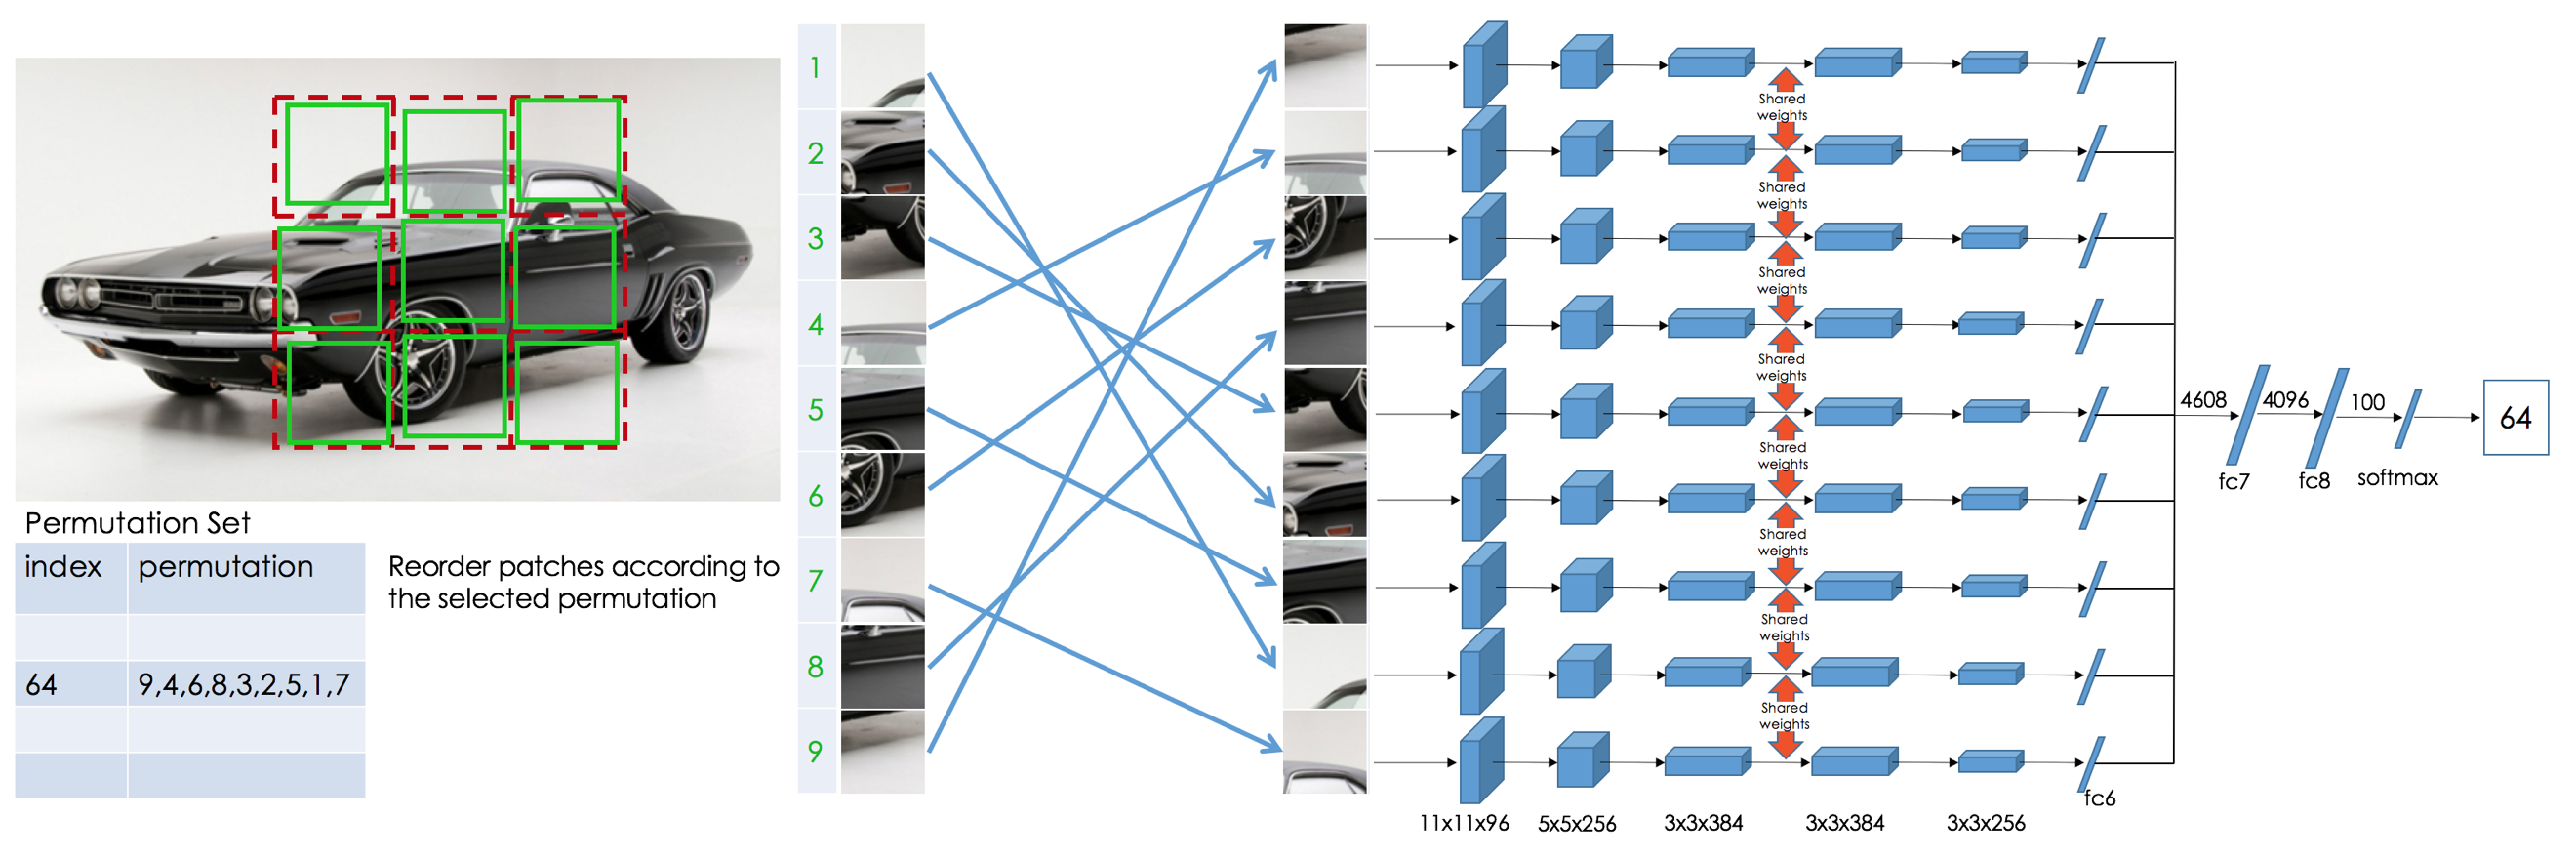
\includegraphics[width=1\textwidth]{Images/Chapter2/jigsaw.png}
\caption{ساختار کلی شبکه‌ی حل پازل}
\label{fig:jigsaw}
\end{figure}

مطالعه‌ی انجام‌شده در این مقاله نشان داد که مدل آموزش‌دیده با این وظیفه‌ی پوششی، قادر به یادگیری بازنمایی‌هایی با کیفیت بالا بوده که در وظایف پایین‌دستی همچون طبقه‌بندی تصویر و شناسایی اشیاء عملکرد قابل توجهی داشته‌اند. همچنین این روش راه را برای توسعه‌ی سایر وظایف زمینه‌محور در یادگیری خودنظارتی هموار ساخت و مبنایی برای کارهای بعدی\cite{li2021jigsawgan,park2024fine} در این حوزه شد. \newline

\noindent\textbf{وظیفه‌ی پوششی پیش‌بینی ترتیب صحیح در دنباله:}

یکی دیگر از وظایف پوششی مبتنی بر زمینه، وظیفه‌ی پیش‌بینی درستی یا نادرستی ترتیب زمانی فریم‌های یک ویدیو است. این وظیفه نخستین بار توسط میسرا و همکارانش در مقاله‌ای با عنوان \lr{Shuffle and Learn} \cite{misra2016shuffle} معرفی شد. ایده‌ی اصلی این روش آن است که فریم‌های استخراج‌شده از یک ویدیو را به‌صورت یک دنباله‌ی تصویری به مدل می‌دهیم و از آن انتظار داریم که تشخیص دهد آیا ترتیب زمانی این فریم‌ها حفظ شده است یا به‌طور تصادفی به هم ریخته شده‌اند. در واقع، این روش یک مسئله‌ی طبقه‌بندی دودویی را تعریف می‌کند که خروجی آن مشخص می‌سازد آیا دنباله‌ی ورودی طبیعی و معنادار است یا نه.

برای افزایش دشواری این وظیفه و در نتیجه به‌دست آوردن بازنمایی‌های باکیفیت‌تر، در مرحله‌ی انتخاب فریم‌ها، از یک راهبرد هوشمندانه بهره گرفته می‌شود. همانطور که در شکل \ref{fig:video-permutation} نشان داده شده است، فریم‌هایی از ویدیو انتخاب می‌شوند که دارای بیشترین تفاوت‌ بصری با یکدیگر هستند. این کار موجب می‌شود مدل نتواند صرفا بر پایه‌ی اطلاعات سطح پایین مانند رنگ یا بافت، تصمیم‌گیری کند، بلکه ناگزیر شود برای تشخیص ترتیب صحیح، به درک عمیق‌تری از محتوای ویدیویی و روابط زمانی میان فریم‌ها برسد.

\begin{figure}[htbp]
\centering
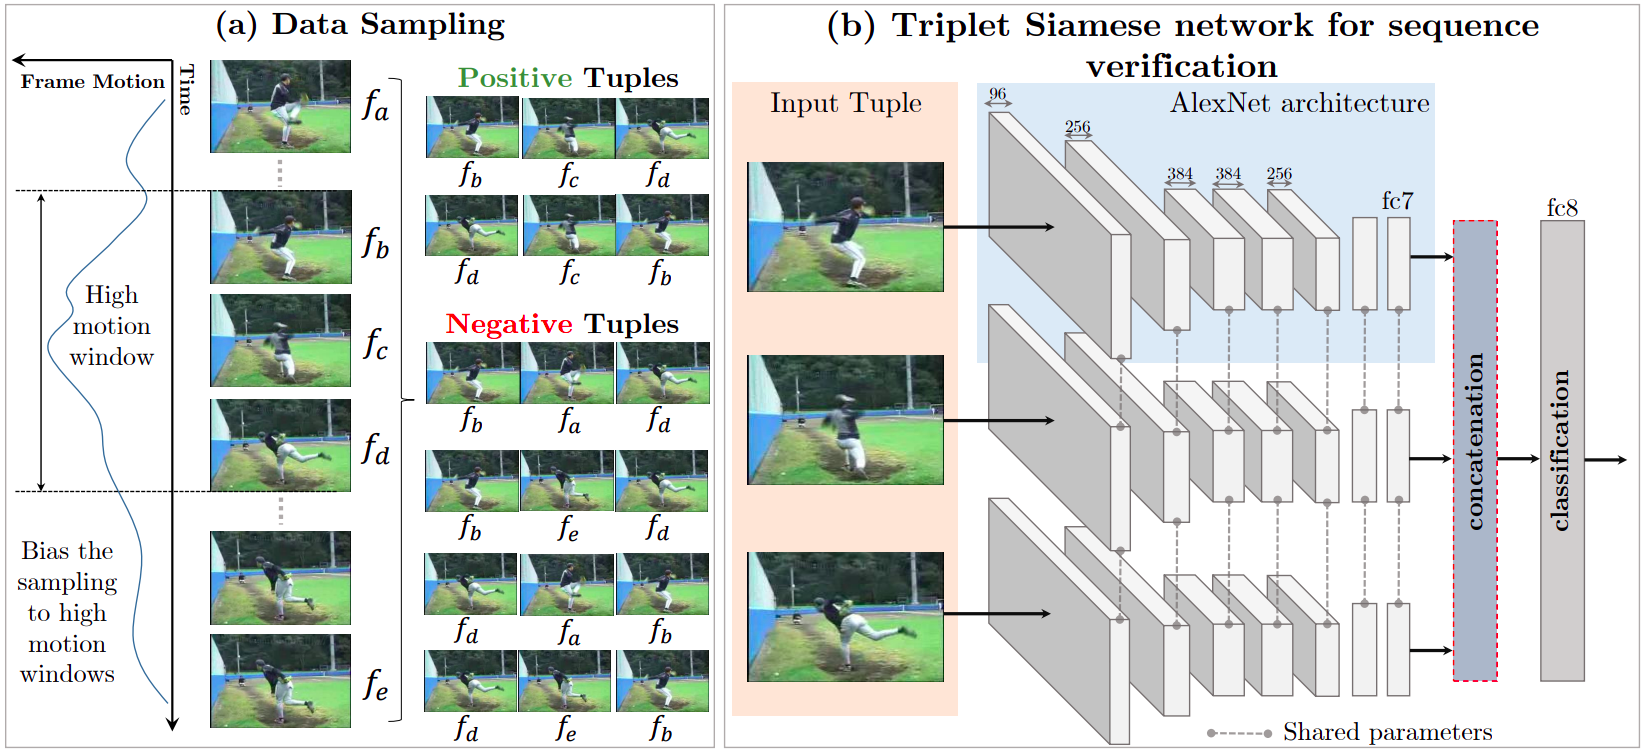
\includegraphics[width=1\textwidth]{Images/Chapter2/video-permutation.png}
\caption{ساختار کلی شبکه‌ی بررسی درستی ترتیب فریم‌های ویدیویی}
\label{fig:video-permutation}
\end{figure}

ساختار کلی شبکه‌ی مورد استفاده نیز شباهت زیادی به روش حل پازل تصویری دارد که پیش‌تر معرفی شد (شکل \ref{fig:jigsaw}). در اینجا نیز از یک شبکه‌ی عصبی برای استخراج ویژگی‌های هر فریم استفاده می‌شود و سپس ویژگی‌های استخراج‌شده در سطحی بالاتر با یکدیگر ترکیب می‌شوند تا تصمیم‌گیری نهایی صورت گیرد. اگرچه این دو روش در ظاهر شباهت‌های زیادی دارند، اما در عمل بر نوع داده‌های متفاوتی تکیه دارند (تصویر در برابر ویدیو) و همچنین اهداف طبقه‌بندی‌شان نیز تفاوت دارد (تشخیص ترتیب صحیح در برابر پیش‌بینی جایگشت دقیق).

علاوه بر داده‌های ویدیویی، این رویکرد در حوزه‌های غیرتصویری نیز مورد استفاده قرار گرفته است. برای مثال، بنویل و همکاران \cite{banville2019self} در مطالعه‌ای بر روی سیگنال‌های مغزی ثبت‌شده با استفاده از الکتروانسفالوگرافی\footnote{الکتروانسفالوگرافی یا نوار مغزی، روشی برای ثبت فعالیت الکتریکی مغز است. در این روش الکترودهایی بر روی پوست سر قرار داده می‌شوند تا امواج مغزی را ثبت کرده و به تشخیص اختلالاتی مانند صرع، مشکلات خواب و آسیب‌های مغزی کمک کنند} (\lr{EEG})،
ایده‌ی تشخیص ترتیب زمانی را به داده‌های چندکاناله‌ی \lr{EEG} تعمیم دادند. این کار نشان می‌دهد که وظایف پوششی مبتنی بر ترتیب، نه تنها در داده‌های بصری، بلکه در داده‌های زمانی پیچیده نیز قابل کاربرد و اثربخش هستند.

\subsubsection{روش‌های بازسازی‌محور}

حال به سراغ دسته‌ی دیگری از روش‌های وظایف پوششی تحت عنوان بازسازی‌محور می‌رویم. در این دسته، ایده‌ی اصلی آن است که مدل با مشاهده‌ی بخشی از داده، یا نسخه‌ای ناقص، فشرده یا مخدوش‌شده‌ی آن، تلاش کند نسخه‌ی کامل یا اصلی داده را بازسازی کند. این فرایند باعث می‌شود مدل ناگزیر به استخراج اطلاعات بنیادی و ساختاری از داده باشد. روش‌های بازسازی‌محور، به‌ویژه در یادگیری نمایش‌های عمیق و قابل انتقال، اهمیت زیادی دارند و بسیاری از آن‌ها با روش‌های مولد نیز همپوشانی دارند؛ چراکه در هر دو، بازتولید داده نقش کلیدی دارد.\newline

\noindent\textbf{خودکدگذارها:}

یکی از نخستین و پایه‌ای‌ترین روش‌های بازسازی‌محور که پایه‌ی بسیاری از دیگر الگوریتم‌های یادگیری خودنظارتی به شمار می‌رود، روش خودر‌مزگذار است. در این چارچوب، یک شبکه‌ی عصبی دو بخشی طراحی می‌شود: بخش نخست، با عنوان کدگذار، داده‌ی ورودی را به یک نمایش فشرده یا بردار ویژگی در فضای نهان نگاشت می‌کند؛ و بخش دوم، یعنی رمزگشا، تلاش می‌کند تا داده‌ی اولیه را از روی همین نمایش بازسازی کند. هدف اصلی، یادگیری یک بازنمایی نهفته است که بتواند ساختارهای اصلی داده را در خود حفظ کرده و بازسازی دقیقی از ورودی ارائه دهد. بدین ترتیب، شبکه بدون نیاز به برچسب‌گذاری، تنها با مشاهده‌ی داده‌های خام و بازسازی آن‌ها، ویژگی‌هایی را می‌آموزد که برای فهم عمیق‌تر محتوا مفید هستند.

روش خودکدگذار را می‌توان یکی از مصداق‌های روشن یادگیری خودنظارتی دانست؛ زیرا وظیفه‌ی آموزشی آن (یعنی بازسازی ورودی) تنها با استفاده از داده‌های خام تعریف می‌شود، بی‌آنکه نیازی به برچسب‌های انسانی باشد. از آن‌جا که خود داده‌ی ورودی نقش برچسب را ایفا می‌کند، ساختار یادگیری آن به‌طور طبیعی در قالب خودنظارتی جای می‌گیرد. این چارچوب، نه‌تنها به‌عنوان یک روش مستقل برای استخراج ویژگی‌های قابل‌انتقال کاربرد دارد، بلکه پایه‌گذار بسیاری از دیگر رویکردهای پیشرفته‌تر مانند خودکدگذار متغیر و خودکدگذار حذف نویز\LTRfootnote{Denoising Auto-Encoder} بوده است.

یکی از گسترش‌های مهم خودکدگذار، خودر‌مزگذار حذف نویز است که برای نخستین بار توسط ونسنت و همکاران \cite{vincent2008extracting} معرفی شد. در این روش، ورودی اصلی به‌صورت مصنوعی دچار اختلال یا نویز می‌شود و مدل موظف است نسخه‌ی اصلی و بدون نویز را بازسازی کند. هدف از این فرایند، واداشتن مدل به یادگیری ویژگی‌هایی مقاوم و پایدار نسبت به اختلالات سطحی داده است. به‌عبارت دیگر، مدل نمی‌تواند صرفا با حفظ جزییات ظاهری داده موفق به بازسازی شود و ناچار است ساختارهای بنیادین‌تری از داده را درک کند. این ویژگی، خودکدگذار حذف نویز را به ابزاری مناسب برای یادگیری نمایش‌های قابل تعمیم در حوزه‌های مختلف مانند بینایی ماشین، پردازش سیگنال و یادگیری انتقالی تبدیل کرده است.\newline


\noindent\textbf{ترمیم تصویر:}

وظیفه پوششی ترمیم تصویر\LTRfootnote{Image Inpainting}
که توسط پاتاک و همکاران\cite{pathak2016context}
ارائه شد، از خودکدگذاری تحت عنوان
کدگذار زمینه‌ای\LTRfootnote{Context Encoder}
استفاده می‌کند تا بتواند یک شبکه‌ی پیچشی را طوری آموزش دهد که بخش‌های حذف‌شده و آسیب‌دیده از تصویر را بازسازی و ترمیم نماید. شبکه برای این که بتواند این وظیفه را به خوبی انجام دهد باید توانایی درک مفاهیم موجود در داده را داشته باشد.
در شکل \ref{fig:inpainting-losses}
یک نمونه از عملکرد این روش را با استفاده از دو تابع هزینه‌ی مختلف می‌توان دید.

\begin{figure}[htb!]
\centering
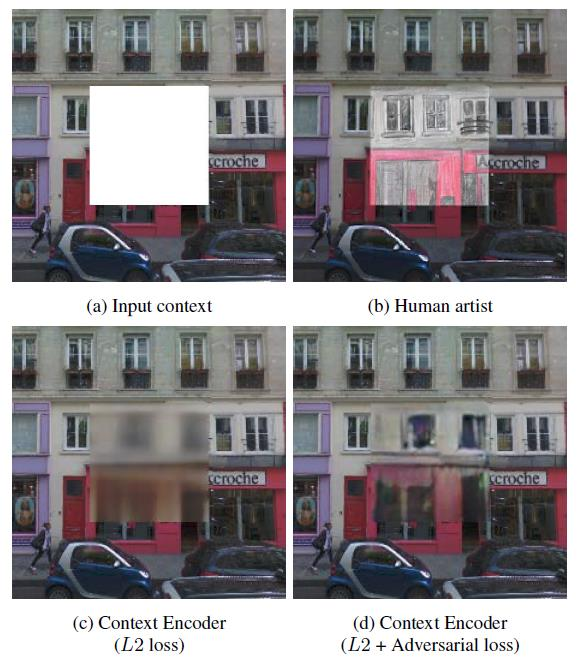
\includegraphics[width=0.7\textwidth]{Images/Chapter2/inpainting-losses.png}
\caption{عملکرد کدگذار زمینه‌ای برای ترمیم تصاویر}
\label{fig:inpainting-losses}
\end{figure}

معماری کلی کدگذار زمینه‌ای این‌گونه است که ابتدا یک یا چند ناحیه از تصاویر را به صورت تصادفی حذف می‌کنیم. این نواحی تصادفی می‌توانند انواع اشکال هندسی مانند دایره و مربع و یا حتی کاملا تصادفی باشد. سپس این تصویر تخریب شده به ورودی شبکه‌ی رمگذار داده می‌شود که معماری کلی آن شباهت زیادی به شبکه‌ی
\lr{AlexNet}
دارد. شبکه‌ی کدگذار یک ماتریس به فرم
$C \times W \times H$
به ازای هر نمونه می‌دهد که در آن $C$ بیانگر تعداد کانال‌ها و $W$ و $H$ بیانگر عرض و ارتفاع ماتریس خروجی هستند. در معماری شبکه‌ی کدگذار زمینه‌ای، برای افزایش ظرفیت یادگیری مدل، خروجی مدل مستقیما به رمزگشا داده نمی‌شود. بلکه از یک لایه‌ی تمام متصل استفاده می‌شود. برای استفاده از لایه‌ی تماما متصل معمولا از
روش‌های ادغام\LTRfootnote{Pooling Methods}
مانند ادغام حداکثر استفاده می‌شود. این‌گونه ابعاد از
$C \times W \times H$
به $C$ تغییر می‌کند.
اما ایراد ادغام این است که می‌تواند اطلاعات باارزش را از بین ببرد. علاوه بر آن اگر بخواهیم که بدون استفاده از ادغام از لایه‌ی تماما متصل استفاده کنیم، باید خروجی را به فرم برداری به طول
$C \times W \times H$
درآوریم که حدود ۱۰۰ میلیون پارامتر به شبکه اضافه می‌کند. این کار علاوه بر پردازش پیچیده، مشکل بیش‌برازش را نیز به‌دنبال خواهد داشت. به‌همین منظور محققان در این مقاله از یک لایه‌ی
تماما متصل درون‌کانالی\LTRfootnote{Channel-wise Fully Connected}
استفاده کردند. بدین صورت که هر یک از
$C$
کانال را به یک بردار به طول
$W \times H$
تبدیل می‌کنیم. سپس یک لایه خواهیم داشت که در دل خود
$C$
لایه‌ی تمام متصل مانند شکل \ref{fig:inpainting-architecture} دارد.
نتیجتا خروجی کدگذار به ورودی رمزگشا همراه با یک لایه‌ی غیر خطی متصل خواهد شد، اطلاعاتی از بین نخواهد رفت و تعداد پارامترهای قابل یادگیری مقدار اندکی افزایش خواهند یافت که برای ما قابل تحمل هستند.

\begin{figure}[htb!]
\centering
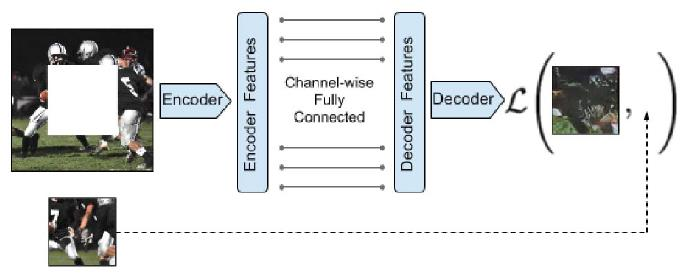
\includegraphics[width=1.0\textwidth]{Images/Chapter2/inpainting-architecture.png}
\caption{معماری کدگذار زمینه‌ای}
\label{fig:inpainting-architecture}
\end{figure}

در رمزگشا با استفاده از لایه‌های
پیچشی معکوس\footnote{منظور از «لایه‌ی پیچشی معکوس»، همان عملیات
\lr{transposed convolution} یا \lr{deconvolution}
است که برای بزرگ‌نمایی ویژگی‌ها در شبکه‌های مولد یا رمزگشا به‌کار می‌رود.}،
ویژگی‌های فشرده شده را به ابعاد تصویر ورودی می‌رسانیم. مثلا ویژگی‌های ورودی به رمزگشا اگر دارای ۶۴ کانال با طول و عرض ۱۶ باشند، آن را به ۳ کانال با طول و عرض ۲۵۶ می‌رسانیم. سپس سیگنال نظارت که همان تصویر سالم است اعمال می‌شود و با استفاده از یک تابع هزینه، آموزش شبکه انجام می‌شود. تابع هزینه‌ی ابتدایی،
میانگین مربعات خطا (\lr{MSE}\LTRfootnote{Mean Squared Error}
می‌باشد
که در فرمول \ref{eq:mse} قابل مشاهده است.
\begin{equation}
    \label{eq:mse}
    L_{rec}(x) = \| \hat{M} \odot (x - F((1 -   \hat{M}) \odot x)) \|_2
\end{equation}
اما همانطور که در شکل \ref{fig:inpainting-losses} بخش \lr{c}
قابل مشاهده است، این تابع هزینه یک خروجی محو شده به ما می‌دهد. محققان برای بهبود خروجی تولید شده از تابع هزینه‌ی تخاصمی استفاده کردند. در واقع از یک شبکه‌ی اضافه تحت عنوان
تفکیک‌کننده\LTRfootnote{Discriminator}
بر پایه‌ی شبکه‌ی مولد تخاصمی استفاده کردند. در اینجا خروجی رمزگشا حکم مولد را خواهد داشت. بنابراین فرمول‌بندی آن به فرم فرمول \ref{eq:adversarial} در می‌آید.
البته در نهایت از ترکیب هزینه‌ی \lr{mse}
و تخاصمی استفاده می‌شود که به فرم فرمول
\ref{eq:combined}
نهایی می‌شود. همانطور که در شکل
\ref{fig:inpainting-losses}
بخش \lr{d}
نیز دیده می‌شود، خروجی دقیق‌تر و بهتری به‌دست می‌آید.
\begin{equation}
    \label{eq:adversarial}
    L_{adv} = \max_{D} \mathbb{E}_{x \in X} [\log(D(x)) + \log(1 - D(F((1 - \hat{M}) \odot x)))]
\end{equation}
\begin{equation}
    \label{eq:combined}
    L = \lambda_{rec} L_{rec} + \lambda_{adv} L_{adv}
\end{equation}
در مقاله، مقدار
$\lambda_{adv}$ برابر با
$0.001$ و مقدار $\lambda_{rec}$ برابر با
$0.999$ قرار داده شده است.
بنابراین هدف اصلی بازتولید دقیق تصویر می‌باشد اما مقدار کمی هزینه‌ی تخاصمی نیز برای وضوح تصاویر تولید شده استفاده شده است.

روش ترمیم تصویر با استفاده از کدگذار زمینه‌ای علاوه بر اینکه وظیفه‌ی اصلی خود یعنی بازسازی نواحی حذف‌شده را انجام می‌دهد، به عنوان یک سیستم پیش‌آموزش قدرتمند برای استخراج ویژگی‌های بصری نیز عمل می‌کند. در حقیقت پس از آموزش کدگذار روی تصاویر بدون برچسب، می‌توان آن را بر روی یک مجموعه داده‌ی دارای برچسب تنظیم دقیق کرد و وظایفی مانند دسته‌بندی را انجام داد.

\subsubsection{یادگیری تباینی}

با وجود پیشرفت‌هایی که روش‌های پیشین یادگیری خودنظارتی در زمان خود به همراه داشتند، همچنان عملکرد آن‌ها فاصله‌ی محسوسی با روش‌های نظارت‌شده کامل داشت. این شکاف عملکردی تا حد زیادی با ظهور یادگیری تباینی در چارچوب یادگیری خودنظارتی کاهش یافت. بهره‌گیری از ایده‌های تباینی منجر به رشد قابل‌توجهی در کیفیت بازنمایی‌های استخراج‌شده از داده‌ها شد، به‌طوری‌که عملکرد مدل‌های بدون‌نظارت در برخی وظایف به سطوح قابل‌مقایسه‌ای با روش‌های نظارت‌شده رسید. در سال‌های اخیر، تمرکز بسیاری از مقالات بر توسعه و بهبود روش‌های خودنظارتی تباینی بر روی انواع داده‌های مختلف از جمله تصویر و سیگنال بوده است. در ادامه، ابتدا به شرح مفهوم یادگیری تباینی پرداخته و سپس برخی از روش‌های شاخص مبتنی بر این رویکرد را مرور می‌کنیم.\newline

\noindent\textbf{تعریف یادگیری تباینی}

یادگیری تباینی در بستر یادگیری خودنظارتی، رویکردی مبتنی بر تمایز است که تلاش می‌کند بازنمایی‌هایی مشابه برای نمونه‌های با مفهوم یکسان و بازنمایی‌هایی متمایز برای نمونه‌های ناهم‌معنا ایجاد کند. این امر معمولاً با بهره‌گیری از تکنیک‌های داده‌افزایی محقق می‌شود؛ به‌این‌ترتیب که از یک داده‌ی واحد چندین نسخه‌ی تغییریافته تولید شده و به‌عنوان نمونه‌های «مثبت» در نظر گرفته می‌شوند، در حالی که داده‌های متفاوت، نمونه‌های «منفی» تلقی می‌گردند. هدف از آموزش مدل، نزدیک کردن بازنمایی نمونه‌های مثبت به یکدیگر و دور ساختن آن‌ها از نمونه‌های منفی است.

برای مثال، فرض کنید از مجموعه داده، دو نمونه‌ی $A$ و $B$ انتخاب می‌شوند و سپس با اعمال داده‌افزایی، نمونه‌های $A_1$ و $B_1$ از آن‌ها ساخته می‌شوند. مدل باید یاد بگیرد که $A$ و $A_1$ را به‌عنوان نمونه‌های مشابه و $A$ و $B_1$ را به‌عنوان نمونه‌های متفاوت در نظر بگیرد. این فرایند با تعریف یک تابع هزینه بر پایه‌ی بردارهای بازنمایی حاصل از یک کدگذار پیاده‌سازی می‌شود (شکل \ref{fig:contrastive}) \cite{jaiswal2020survey}. در نهایت، کدگذار آموزش‌دیده قادر خواهد بود بازنمایی‌هایی غنی و قابل‌انتقال برای استفاده در وظایف یادگیری پایین‌دستی فراهم آورد.

\begin{figure}[htb!]
\centering
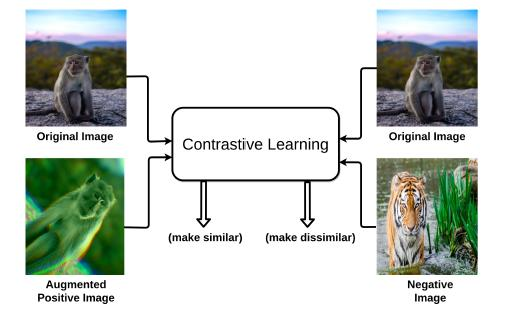
\includegraphics[width=0.7\textwidth]{Images/Chapter2/contrastive.png}
\caption{نمونه‌ای از فرایند یادگیری تباینی}
\label{fig:contrastive}
\end{figure}

در ادامه به بررسی تعدادی از روش‌ها و مقالات منتشر شده در این حوزه می‌پردازیم.\newline

\noindent\textbf{روش کدگذاری پیش‌بینی‌کننده‌ی تباینی (\lr{CPC\LTRfootnote{Contrastive Predictive Coding}})}\label{sec:CPC}

روش کدگذاری پیش‌بینی‌کننده‌ی تباینی یا به اختصار \lr{CPC}
که نخستین بار در سال ۲۰۱۸ توسط
\lr{Oord}
و همکاران\cite{oord2018representation}
معرفی شد، یکی از اولین تلاش‌های موفق برای استفاده از یادگیری تباینی در استخراج بازنمایی‌های غنی و قابل انتقال از داده‌های بدون برچسب بود. این روش، به‌ویژه در داده‌های ترتیبی مانند صوت و سیگنال، عملکرد قابل‌توجهی از خود نشان داده و در حوزه‌هایی مانند تشخیص گفتار کاربرد یافته است.

ایده‌ی اصلی این روش بر پایه‌ی پیش‌بینی اطلاعات آینده از روی گذشته است. اما بر خلاف بسیاری از دیگر روش‌های
خودهمبسته\LTRfootnote{Autoregressive}
که آینده را با تولید داده‌ی اصلی پیش‌بینی می‌کنند، یک مدل مولد نیست. بلکه یک مدل تباینی است که هدف آن پیش‌بینی بازنمایی مربوط به آینده با استفاده از تابع هزینه تباینی است.

\begin{figure}[htb!]
\centering
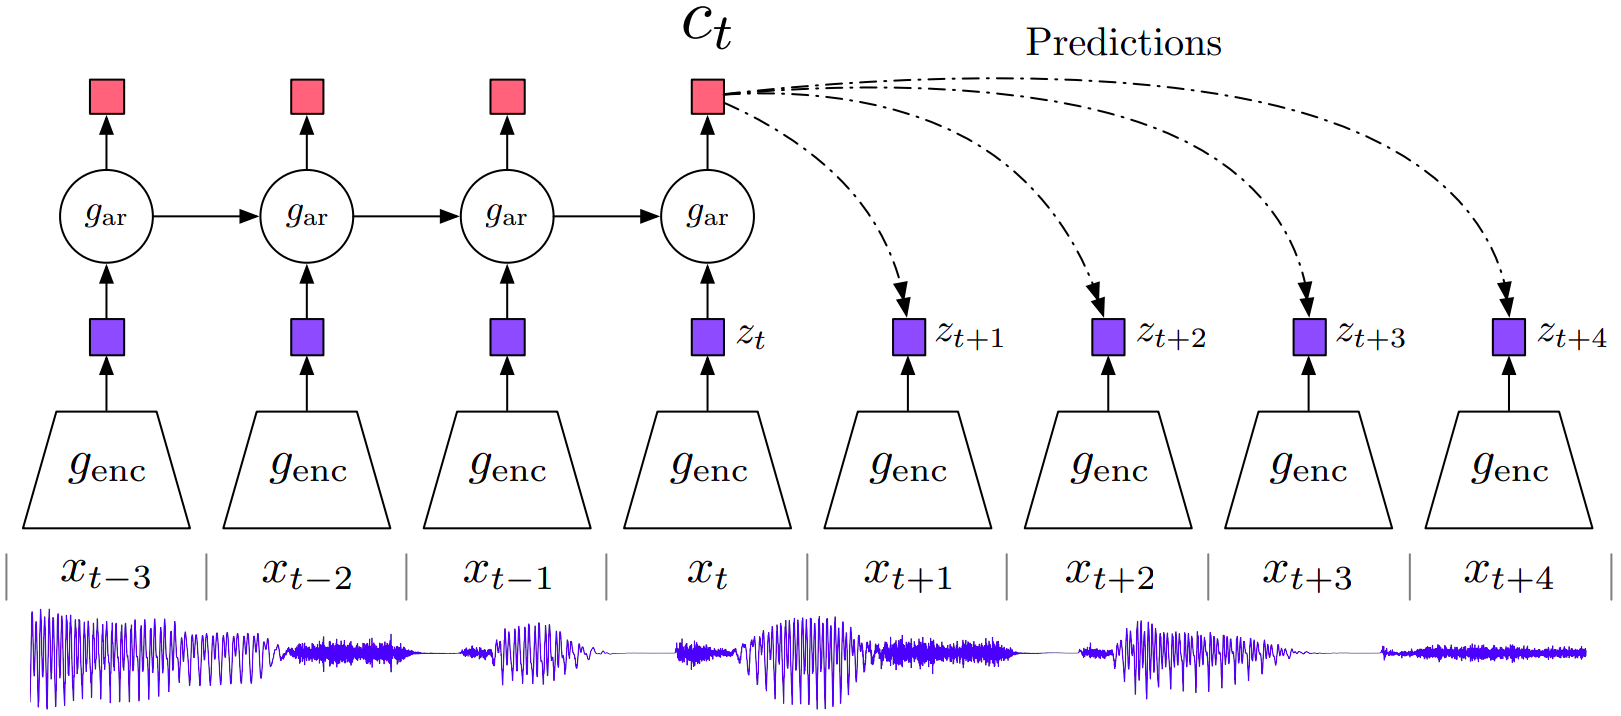
\includegraphics[width=1\textwidth]{Images/Chapter2/cpc.png}
\caption{ساختار کلی روش \lr{CPC}}
\label{fig:cpc}
\end{figure}

با این فرض که مجموعه داده ورودی سری زمانی می‌باشد،
فرض کنید در $x_t$ هستیم
که هر $x_t$
بیانگر یک پنجره از سری زمانی می‌باشد که می‌تواند دارای همپوشانی با پنجره‌های مجاور باشد. با استفاده از یک شبکه‌ی پیچشی ($g_{enc}$)، بردارهای بازنمایی برای پنجره‌های از
$x_{t-n}$ تا $x_t$ می‌سازیم.
سپس با استفاده از یک شبکه‌ی بازگشتی مانند واحد بازگشتی دروازه‌ای ($g_{ar}$)،
از روی
$g_{enc}(x_{t-n})$ تا $g_{enc}(x_t)$
یک بردار زمینه تحت عنوان $c_t$
تولید می‌کنیم.

حال به نوآوری این روش می‌رسیم. در روش \lr{CPC}
به‌جای این که از بردار $c_t$
برای تخمین مستقیم توزیع احتمالاتی $k$ قدم آینده استفاده شود
(یعنی $p_k(x_{t+k}|c_t)$)،
از یک نسبت چگالی\LTRfootnote{Density Ratio}
استفاده می‌شود که هدف آن حفظ اطلاعات متقابل بین بازنمایی آینده
$z_{t+k}$ و بردار زمینه $c_t$ است.
این نسبت چگالی به‌صورت معادله \ref{eq:density-ratio} مدل‌سازی می‌شود
که در آن تابع امتیازدهی $f_k$
میزان شباهت بازنمایی آینده و زمینه را نشان می‌دهد. برای پیاده‌سازی، از یک مدل ساده به فرم
معادله \ref{eq:density-ratio-simple}
استفاده شده است که در آن $W_k$
یک ماتریس تبدیل خطی قابل آموزش برای گام زمانی $k$ است.
این مدل با محاسبه‌ی شباهت بین بردار
$z_{t+k}$
(که یک نماینده‌ی بازنمایی برای آینده است)
و بردار زمینه‌ی $c_t$،
تلاش می‌کند که امتیاز را برای
$z_{t+k}$های مثبت بیشینه
و برای $z_{t+k}$های منفی کمینه کند
\begin{equation}
\label{eq:density-ratio}
f_k(z_{t+k}, c_t) \propto \frac{p(z_{t+k}|c_t)}{p(z_{t+k})}
\end{equation}
\begin{equation}
\label{eq:density-ratio-simple}
f_k(z_{t+k}, c_t) = \exp \left( z_{t+k}^T W_k c_t \right)
\end{equation}
برای آموزش مدل، از تابع هزینه‌ی
\lr{InfoNCE\LTRfootnote{Information Noise-Contrastive Estimation}} به فرم معادله‌ی \ref{eq:infonce}
استفاده می‌شود که در آن $X$ شامل $N$
نمونه‌ی تصادفی است که یکی از آن‌ها نمونه‌ی مثبت و $N-1$
تای دیگر نمونه‌های منفی هستند. هدف مدل این است که امتیاز شباهت $f_k$
برای نمونه‌ی واقعی نسبت به نمونه‌های منفی بیشتر باشد. بدین ترتیب، مدل می‌آموزد که بازنمایی $c_t$
شامل اطلاعات مفیدی برای پیش‌بینی آینده‌ی داده باشد.
\begin{equation}
\label{eq:infonce}
\mathcal{L}_N = - \mathbb{E}_X \left[ \log \frac{f_k(x_{t+k}, c_t)}{\sum_{x_j \in X} f_k(x_j, c_t)} \right]
\end{equation}
در نهایت، پس از پایان مرحله‌ی پیش‌‌آموزش، می‌توان از کدگذار آموزش‌دیده به‌عنوان یک استخراج‌کننده‌ی ویژگی استفاده کرد و بازنمایی‌های به‌دست‌آمده را در وظایف پایین‌دستی مانند دسته‌بندی به‌کار برد.\newline

\noindent\textbf{استفاده از بانک حافظه\LTRfootnote{Memory Bank} و تکانه\LTRfootnote{Momentum}:}

یکی از چالش‌های اصلی در پیاده‌سازی موثر یادگیری تباینی، نیاز به مجموعه‌ای بزرگ و متنوع از نمونه‌های منفی است. برای اینکه مدل بتواند تمایز درستی بین نمونه‌های مثبت و منفی قائل شود، باید در هر تکرار آموزشی تعداد زیادی نمونه‌ی منفی داشته باشد. این در حالی است که در یک دسته از ورودی، تنها تعداد محدودی از نمونه‌ی منفی در دسترس است. به همین منظور، محققان روشی تحت عنوان
بانک حافظه\cite{wu2018unsupervised}
را ارائه دادند.

در این روش، به‌جای آن که فقط از داده‌های موجود در دسته‌ی ورودی فعلی استفاده شود، یک بردار بازنمایی برای هر نمونه در کل مجموعه داده محاسبه و در یک بانک حافظه ذخیره می‌شود. در طول آموزش، این بانک به‌طور تدریجی به‌روزرسانی شده و از آن برای استخراج نمونه‌های منفی استفاده می‌شود. فرض اصلی این روش (مانند بیشتر روش‌های دیگر تباینی) این است که هر نمونه در مجموعه داده به‌عنوان یک کلاس منحصربه‌فرد در نظر گرفته شود و بنابراین یادگیری بازنمایی به‌صورت تباینی بر اساس تفاوت بین نمونه‌ها صورت می‌گیرد.
\begin{equation}
\label{eq:membank-infonce}
\mathcal{L}_i = -\log \frac{\exp(z_i^\top v_i / \tau)}{\sum_{j=1}^{K} \exp(z_i^\top v_j / \tau)}
\end{equation}

تابع هزینه به‌کاررفته در این روش به فرم معادله‌ی \ref{eq:membank-infonce}
می‌باشد که همان تابع هزینه‌ی \lr{InfoNCE}
می‌باشد. در این فرمول:
\begin{itemize}
    \item $z_i$ بردار بازنمایی نمونه‌ی ورودی است که توسط شبکه کدگذار تولید شده است.
    \item $v_i$ بازنمایی ذخیره شده‌ی همان نمونه در بانک حافظه است (مثبت).
    \item $v_j$ دیگر نمونه‌های استخراج‌شده از بانک حافظه‌اند.
    \item $\tau$ پارامتر دما است که بسته به مقدار آن باعث هموارسازی یا تیزکردن نمودار خروجی می‌شود.
\end{itemize}
با وجود عملکرد قابل قبول، یکی از مشکلات این روش آن است که بانک حافظه به‌صورت مستقیم از پارامترهای کدگذار فعلی به‌روزرسانی نمی‌شود و در طول آموزش بین بازنمایی‌های فعلی و آنچه در حافظه ذخیره شده، ناسازگاری‌هایی به‌وجود خواهد آمد. این موضوع می‌تواند مانع از یادگیری پایدار شود.

در راستای رفع مشکل ناهماهنگی بانک حافظه، روش تباین تکانه یا به اختصار
\lr{Moco\LTRfootnote{Momentum Contrast}}
توسط \lr{He} و همکاران\cite{he2020momentum} معرفی شد.
ایده‌ی اصلی این روش استفاده از دو شبکه کدگذار است؛
یک کدگذار جستار\LTRfootnote{Query Encoder}
و یک کدگذار کلید\LTRfootnote{Key Encoder}.
کدگذار جستار مستقیما از طریق پس‌انتشار به‌روزرسانی می‌شود؛ در حالی که کدگذار کلید با استفاده از به‌روزرسانی تکانه‌ای روی کدگذار جستار به‌روزرسانی می‌شود. فرم به‌روزرسانی تکانه‌ای برای پارامترهای کدگذار کلید به شکل زیر تعریف می‌شود:
\begin{equation}
\theta_k \leftarrow m \cdot \theta_k + (1 - m) \cdot \theta_q
\end{equation}
که در آن:
\begin{itemize}
    \item $\theta_q$ پارامترهای کدگذار جستار است.
    \item $\theta_k$ پارامترهای کدگذار کلید است.
    \item $m$ ضریب تکانه است که با قرار دادن مقادیر نزدیک به ۱ (در مقاله برابر با $0.999$ می‌باشد) باعث می‌شود تغییرات پارامترهای کلید آهسته‌تر و پیوسته‌تر باشد.
\end{itemize}
\begin{figure}[htb!]
\centering
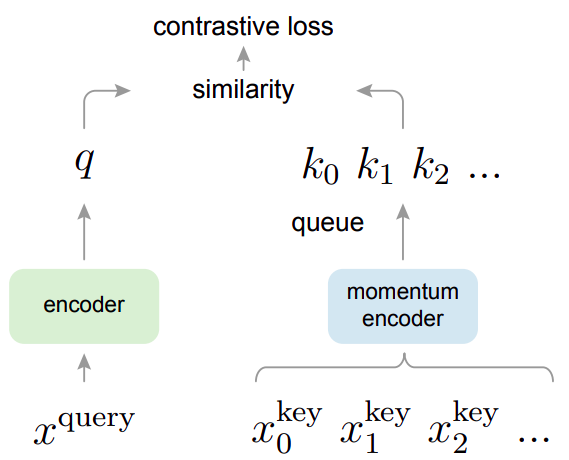
\includegraphics[width=0.6\textwidth]{Images/Chapter2/moco.png}
\caption{ساختار کلی روش \lr{MoCo}}
\label{fig:moco}
\end{figure}
از طرفی، \lr{MoCo}
به‌جای استفاده از یک بانک حافظه‌ی کامل که تمام داده‌ها را نگهداری می‌کند،
از یک صف حافظه\LTRfootnote{Queue}
استفاده می‌کند. در این صف، بازنمایی‌های کلید تولید شده از نمونه‌های قبلی ذخیره می‌شوند. به‌مرور زمان، نمونه‌های قدیمی از صف خارج شده و نمونه‌های جدید جای آن‌ها را می‌گیرند. این ساختار حافظه‌ی پویا، ضمن صرفه‌جویی در حافظه، امکان دسترسی به هزاران نمونه‌ی منفی را در هر تکرار آموزشی فراهم می‌کند. تابع هزینه مورد استفاده در \lr{MoCo}
نیز نوعی از \lr{InfoNCE} است:
\begin{equation}
\mathcal{L}_q = -\log \frac{\exp(q \cdot k^+ / \tau)}{\sum_{i=0}^{K} \exp(q \cdot k_i / \tau)}
\end{equation}
که در آن:
\begin{itemize}
    \item $q$ بازنمایی حاصل از کدگذار جستار است.
    \item $k^+$ نمونه‌های مثبت تولید شده توسط کدگذار کلید است
    \item $k_i$ نمونه‌های منفی ذخیره‌شده در صف حافظه هستند.
    \item $\tau$ پارامتر دما است.
\end{itemize}
روش \lr{MoCo}
به‌دلیل استفاده از کدگذار کلید با به‌روزرسانی تکانه‌ای، انسجام میان بازنمایی‌های فعلی و نمونه‌های منفی ذخیره‌شده را حفظ می‌کند و در عین حال بدون نیاز به پردازش مجدد تمام داده‌ها، بازنمایی‌های به‌روز و موثری تولید می‌نماید. این مدل باعث پایداری بیشتر آموزش و بهبود دقت مدل‌های پیش‌آموزش‌یافته شد.\newline

\noindent\textbf{یادگیری تباینی ساده اما قدرتمند: روش \lr{SimCLR}}\label{sec:simclr}

روش یادگیری تباینی ساده که به‌اختصار
\lr{SimCLR\LTRfootnote{Simple Framework for Contrastive Learning of Visual Representations}}
نامیده می‌شود، یکی از اثرگذارترین و پایه‌ای‌ترین روش‌های یادگیری تباینی خودنظارتی است که توسط
چن و همکاران\cite{chen2020simple}
معرفی شد. برخلاف روش‌هایی مانند
\lr{MoCo}
که به ساختارهای پیچیده‌ای نظیر صف حافظه و کدگذار تکانه‌ای نیاز دارند،
\lr{SimCLR}
با ساختاری بسیار ساده، توانست بازنمایی‌های قدرتمندی را برای تصاویر یاد بگیرد و عملکرد قابل مقایسه با روش‌های نظارت‌شده به‌دست آورد. سادگی معماری در کنار داده‌افزایی قوی و دسته‌های بزرگ داده آموزشی کلید عملکرد خوب این روش است.

فرایند آموزش در \lr{SimCLR}
از چهار جزء اصلی تشکیل شده است:
\begin{enumerate}
    \item داده‌افزایی قوی
    \item شبکه کدگذار
    \item شبکه نگاشت\LTRfootnote{Projection Head}
    \item تابع هزینه \lr{InfoNCE}
\end{enumerate}

در ادامه هر یک از این اجزا را بررسی می‌کنیم.

\noindent\textbf{داده‌افزایی قوی:}
دو تابع داده‌افزایی به‌صورت تصادفی بر روی هر ورودی $xـk$
اعمال می‌شود و در نتیجه‌ی آن دو نمایش
$x_{2k-1}$ و $x_{2k}$ تولید می‌گردند.
ترکیب‌های متعددی از تابع‌های تبدیل مختلف موجود در شکل
\ref{fig:simclr-augmentations}
به‌صورت تصادفی می‌توانند استفاده شوند تا خروجی‌های مختلف و تصادفی برای هر داده ایجاد شوند. برای مثال یکی از توابع مورد استفاده می‌تواند به‌این صورت باشد که با یک احتمال برش انجام دهد، با یک احتمال تصویر را قرینه و برعکس کند، نویز تصادفی گوسی با میانگین
$\mu$ و انحراف معیار $\sigma$
اعمال کند و رنگ تصویر را به‌صورت تصادفی تغییر دهد. نتیجتا با دو بار اعمال این تابع تصادفی بر روی هر ورودی، دو داده‌ی افزوده خواهیم داشت که باید شباهتشان را با یکدیگر بیشینه کنیم. هر چه شدت اعمال روش‌های افزایش داده بیشتر باشد، تفکیک بین داده‌های مثبت و منفی را برای مدل سخت‌تر می‌کند؛ اما همین امر می‌تواند باعث شود که مدل وادار به یادگیری بازنمایی‌های مفیدتر و کاربردی‌تر شود. همچنین هر چه تعداد نمونه‌های منفی درون یک دسته‌ی آموزشی بیشتر باشد، مدل نمونه‌های بیشتری را می‌بیند و به‌همین ترتیب تباین بهتری می‌تواند انجام دهد و یادگیری قوی‌تر و پایدارتر می‌شود.
\begin{figure}[t!]
\centering
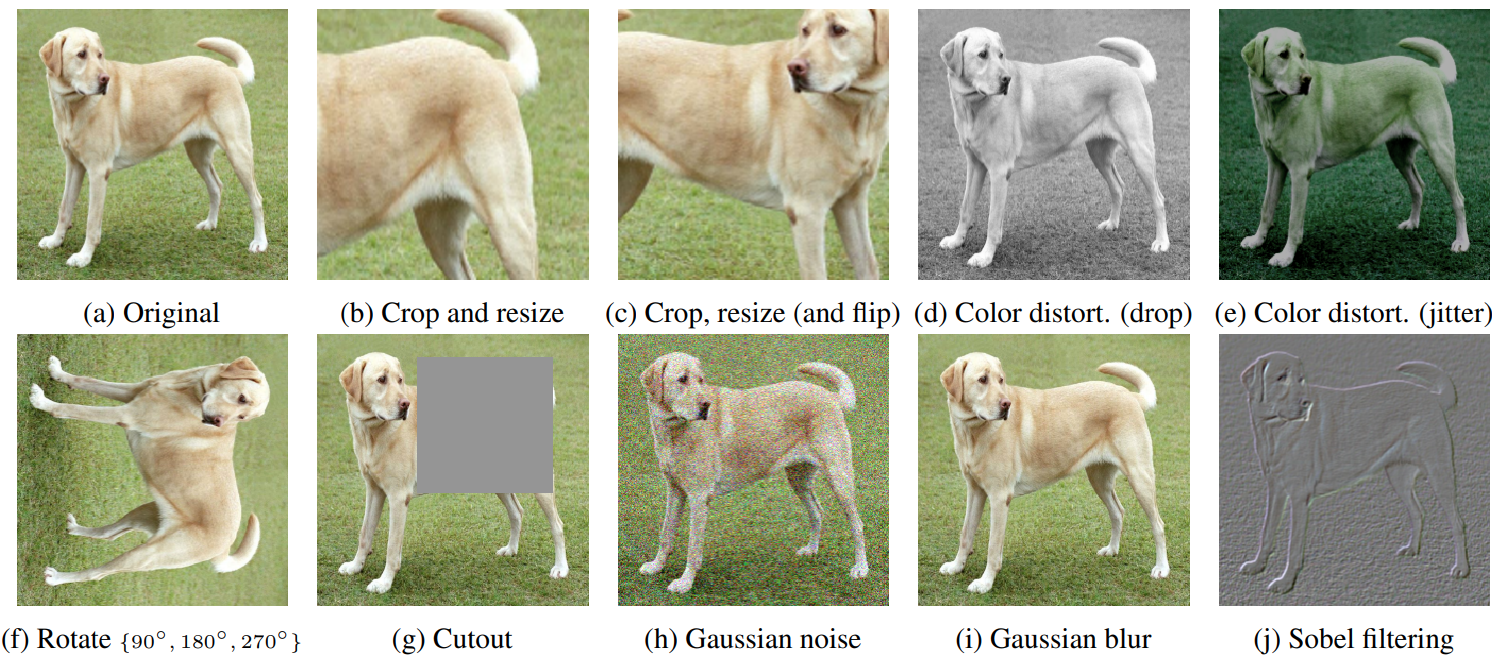
\includegraphics[width=1\textwidth]{Images/Chapter2/simclr-augmentations.png}
\caption{روش‌های ایجاد داده‌ی افزوده}
\label{fig:simclr-augmentations}
\end{figure}

\noindent\textbf{شبکه کدگذار:}
برای هر نما $x_\ell$،
با استفاده از کدگذار $f_\theta$ مبتنی بر شبکه‌ی پیچشی،
یک بردار بازنمایی $h_\ell$
به فرم معادله \ref{eq:simclr-encoder} می‌سازیم.
\begin{equation}
\label{eq:simclr-encoder}
h_\ell = f_\theta(x_\ell)\in\mathbb{R}^d
\end{equation}
در مقاله، از یک شبکه \lr{ResNet}
بدون لایه‌ی دسته‌بندی کننده استفاده شده است و
$h_\ell$
بعد از تجمیع سراسری به‌دست می‌آید. در ارزیابی پایین‌دستی از همین $h$
به‌عنوان بازنمایی نهایی برای هر نمونه استفاده می‌شود.

\noindent\textbf{شبکه نگاشت:}
یکی از نوآوری‌های روش \lr{SimCLR}،
استفاده از یک شبکه تماما متصل کم‌عمق (یک لایه پنهان) تحت عنوان شبکه نگاشت می‌باشد. با استفاده از این شبکه، خروجی $h_\ell$
تبدیل به $z_\ell$ می‌شود.
\begin{equation}
\label{eq:simclr-projection}
\boldsymbol{z}_\ell = g_\phi(\boldsymbol{h}_\ell) = \boldsymbol{W}^{(2)} \sigma(\boldsymbol{W}^{(1)} \boldsymbol{h}_\ell)
\end{equation}
نویسندگان مقاله نشان دادند که استفاده از یک شبکه نگاشت و یک تابع فعال‌ساز غیر خطی و سپس اعمال هزینه‌ی تباینی بر روی
$z$
عملکرد بهتری را نسبت به استفاده از
$h$
برای محاسبات هزینه‌ی تباینی می‌دهد. ایده‌ی شهودی برای این کار این است که
$g_\phi$
جذب‌کننده‌ی هزینه‌ی تباینی باشد تا
$f_\theta$
بازنمایی‌های عمومی‌تری را بیاموزد.
در معادله \ref{eq:simclr-projection}،
$W^{(1)}$ و $W^{(2)}$ پارامترهای شبکه‌ی نگاشت و
$\sigma$ تابع فعال‌ساز غیر خطی می‌باشد که معمولا از تابع \lr{ReLU\LTRfootnote{Rectified Linear Unit}} استفاده می‌شود.

\noindent\textbf{تابع هزینه تباینی:}
فرض کنید یک دسته آموزشی شامل $N$
نمونه ورودی باشد. پس با دو نما از هر تصویر،
$2N$
نمونه آموزشی خواهیم داشت. سپس برای دو نمونه‌ی مثبت $i$ و $j$ معادله
\ref{eq:simclr-loss} را خواهیم داشت.
\begin{equation}
\label{eq:simclr-loss}
    \ell_{i,j} = -\log \frac{\exp(sim(\boldsymbol{z}_i, \boldsymbol{z}_j) / \tau)}{\sum_{k=1}^{2N} 1_{[k \neq i]} \exp(sim(\boldsymbol{z}_i, \boldsymbol{z}_k) / \tau)}
\end{equation}
\begin{equation}
    \label{eq:simclr-cosine}
    sim(\boldsymbol{u}, \boldsymbol{v}) = \boldsymbol{u}^\top \boldsymbol{v} / \|\boldsymbol{u}\| \|\boldsymbol{v}\|
\end{equation}
\begin{figure}[t]
\centering
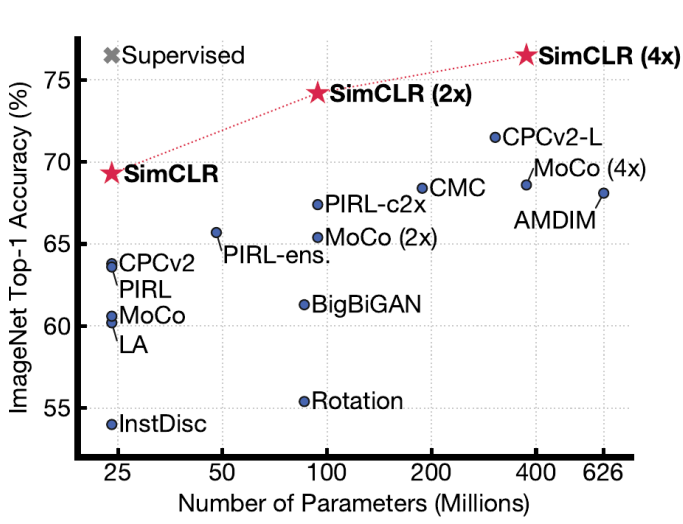
\includegraphics[width=0.6\textwidth]{Images/Chapter2/simclr-results.png}
\caption{دقت روش \lr{SimCLR}}
\label{fig:simclr-results}
\end{figure}
در این معادله،
$1_{[k \neq i]}\in\{0,1\}$
بیانگر تابع نشانگر\LTRfootnote{Indicator function}
می‌باشد که برای تمامی $k$ها
نابرابر با $i$
برابر با یک می‌باشد.
پارامتر $\tau$
تمرکز توزیع را کنترل می‌کند. هر چه
$\tau$
کوچک‌تر، شیب‌ها تیزتر
تابع $sim$
نیز بیانگر یک معیار سنجش شباهت بین نمونه‌ها می‌باشد. در مقاله اصلی از تابع
شباهت کسینوسی\LTRfootnote{Cosine Similarity}
استفاده شده که فرمول آن به فرم معادله
\ref{eq:simclr-cosine} می‌باشد.
شباهت کسینوسی بیانگر کسینوس زاویه‌ی بین دو بردار می‌باشد. هر چه دو بردار در یک جهت باشند، کسینوس زاویه‌ی بین آن‌ها بیشینه و به یک نزدیک می‌شود و هر چه در خلاف جهت یکدیگر باشند، کسینوس زاویه‌ی بین آن‌ها کمینه و به  منفی یک نزدیک می‌شود. بنابراین این تابع هزینه
$f_\theta$ و به تبع آن $g_\phi$
را وادار می‌کند که نگاشت مربوط به نمونه‌های مثبت در یک جهت قرار گیرند و تا جای ممکن در جهت مخالف نسبت به دیگر نمونه‌های دسته باشند.

تابع هزینه استفاده شده در معادله \ref{eq:simclr-loss}،
آنتروپی متقاطع نرمال‌شده با مقیاس دمایی
(\lr{NT-Xent}\LTRfootnote{Normalized Temperature-scaled Cross-Entropy loss}) است که فرمی از تابع \lr{InfoNCE}
می‌باشد. می‌توان نشان داد که با افزایش تعداد منفی‌ها و کمینه کردن این هزینه، کران پایین روی
اطلاعات متقابل\LTRfootnote{Mutual Information}
بین نماها افزایش می‌یابد. یعنی این که با کمینه کردن این تابع هزینه هنگامی که از تعداد نمونه‌های زیادی در یک دسته استفاده کرده‌ایم، مدل یاد می‌گیرد که اطلاعات متقابل بین نمونه‌های مثبت را افزایش دهد و در واقع بازنمایی‌های پایدارتر و کاربردی‌تری را از روی داده‌ها بیاموزد.
\begin{table}[t]
\centering
\caption{دقت روش \lr{SimCLR} در یادگیری انتقالی}
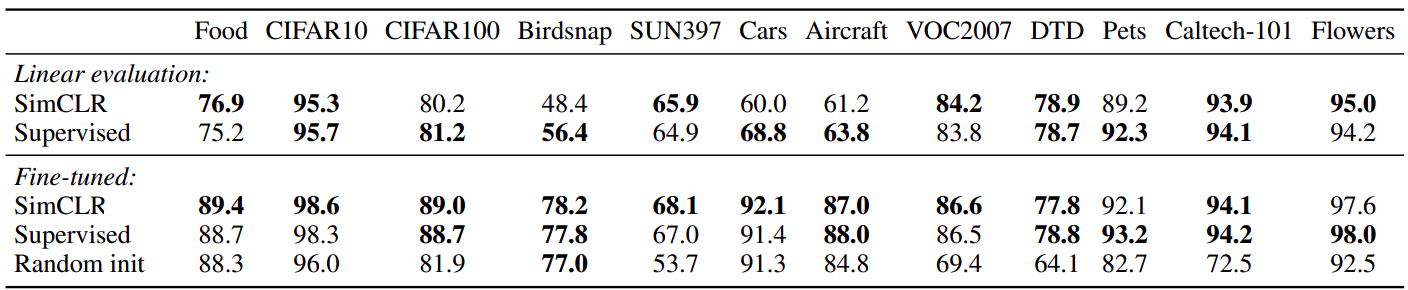
\includegraphics[width=1\textwidth]{Images/Chapter2/simclr-transfer.png}
\label{tab:simclr-transfer}
\end{table}
در نهایت پس از پایان پیش‌آموزش مدل، شبکه‌ی نگاشت به‌کل کنار گذاشته می‌شود چرا که برای وظیفه‌ی یادگیری تباینی و هزینه‌ی \lr{NT-Xent}
آموزش دیده بود. سپس یک شبکه‌ی تماما متصل دیگر به‌عنوان یک دسته‌بند به‌جای شبکه‌ی نگاشت قرار داده می‌شود و یادگیری را بر روی مجموعه داده برچسب‌دار انجام می‌دهیم.

همانطور که در شکل \ref{fig:simclr-results}
می‌توان دید، با افزایش پارامترها دقت روش \lr{SimCLR}
بهبود بسیاری یافته؛ تا جایی که به دقت روش نظارت‌شده رسیده و قابل مقایسه با آن شده است. اما نکته‌ی بسیار مهم روش \lr{SimCLR}
قابلیت تعمیم‌پذیری آن است. همانطور که در جدول \ref{tab:simclr-transfer}
می‌توان دید، عملکرد روش \lr{SimCLR}
در یادگیری انتقالی با روش‌های نظارت‌شده برابری می‌کند و در بسیاری از موارد از آن‌ها پیشی گرفته است.

\subsubsection{پردازش زبان طبیعی}
پردازش زبان طبیعی\LTRfootnote{Natural Language Processing - NLP} یکی از مهم‌ترین شاخه‌های هوش مصنوعی است که هدف آن تعامل مؤثر میان انسان و ماشین از طریق زبان طبیعی می‌باشد. در سال‌های اخیر، یادگیری خودنظارتی پیشرفت‌های شگرفی را در این حوزه رقم زده است. این رویکرد با بهره‌گیری از حجم عظیمی از داده‌های بدون برچسب و تعریف وظایف پیش‌بینی کمکی (مانند پیش‌بینی واژه‌های حذف‌شده یا پیش‌بینی جمله‌ی بعدی) و همچنین با بهره‌گیری از مدل مبدل\LTRfootnote{Transformer}\cite{vaswani2017attention}، امکان یادگیری نمایش‌های زبانی قدرتمند و غنی را فراهم ساخته است. مزیت اصلی این روش در مقایسه با یادگیری نظارت‌شده، عدم نیاز به برچسب‌گذاری دستی داده‌ها و قابلیت تعمیم بهتر مدل به وظایف گوناگون زبان طبیعی است. ظهور مدل‌هایی همچون \lr{BERT\LTRfootnote{Bidirectional Encoder Representations from Transformers}} و \lr{GPT\LTRfootnote{Generative Pre-Trained Transformer}}، که بر مبنای یادگیری خودنظارتی آموزش دیده‌اند، باعث ایجاد جهشی چشمگیر در کیفیت حل مسائل متنوع پردازش زبان طبیعی مانند ترجمه ماشینی، درک مطلب، و تولید متن شده است. علاوه بر این، استفاده از تمام داده‌های متنی موجود در آموزش، این امکان را فراهم می‌کند که اندازه و ظرفیت مدل (تعداد پارامترها) را به‌طور قابل‌توجهی افزایش دهیم، بی‌آن‌که به‌سادگی دچار بیش‌برازش شویم. این رویکرد منجر به پیدایش نسل جدیدی از مدل‌ها شده که با نام مدل‌های زبانی بزرگ (\lr{LLM\LTRfootnote{Large Language Models}}) شناخته می‌شوند و قادرند طیف گسترده‌ای از وظایف زبانی را تنها با یک فرایند آموزش عمومی، بدون نیاز به بازآموزی ویژه، انجام دهند. در ادامه، دو مدل \lr{BERT} و \lr{GPT} به‌عنوان نمونه‌های شاخص این رویکرد مورد بررسی قرار می‌گیرند.\newline

\noindent\textbf{مدل \lr{BERT}}

مدل \lr{BERT} که توسط \lr{Devlin} و همکاران\cite{devlin2019bert} معرفی شد،
یک معماری بر مدل مبدل است که با هدف یادگیری بازنمایی‌های زبانی عمیق و دوسویه طراحی شده است. بر خلاف مدل‌های پیشین که جهت پردازش را محدود به چپ‌به‌راست یا راست‌به‌چپ می‌کردند،
\lr{BERT}
از خودتوجهی دوسویه\LTRfootnote{Bidirectional Self-attention}
بهره می‌گیرد و در هر لایه به تمام کلمات موجود در جمله، هم از سمت چپ و هم از سمت راست، توجه می‌کند. این ویژگی باعث می‌شود که مدل بتواند وابستگی‌های معنایی پیچیده را به‌شکل دقیق‌تری مدل‌سازی کند.

مدل \lr{BERT} با استفاده از دو وظیفه‌ی پوششی آموزش داده می‌شود:
\begin{enumerate}
    \item \textbf{وظیفه مدل‌سازی زبان پوشیده\LTRfootnote{Masked Language Modeling}:}
    در این روش، درصدی از توکن‌های ورودی به‌صورت تصادفی با یک نشانه ویژه جایگزین می‌شوند و مدل باید با استفاده از بافت دوطرفه، توکن‌های پوشیده را پیش‌بینی کند. این کار باعث می‌شود که مدل به‌طور همزمان از اطلاعات گذشته و آینده در جمله بهره ببرد.
    \item \textbf{وظیفه پیش‌بینی جمله بعدی:}
    در این وظیفه، به مدل دو جمله ارائه می‌شود و مدل باید تشخیص دهد که آیا جمله دوم واقعا در متن اصلی پس از جمله اول آمده یا خیر. این مرحله به \lr{BERT} کمک می‌کند تا روابط سطح جمله و انسجام متنی را بیاموزد.
\end{enumerate}
پس از پیش‌آموزش، \lr{BERT} می‌تواند برای طیف وسیعی از وظایف زبانی مانند دسته‌بندی متون، پاسخ به پرسش، برچسب‌گذاری توالی و استنتاج معنایی تنظیم دقیق شود.\newline

\noindent\textbf{مدل \lr{GPT}}

مدل‌های \lr{GPT}\cite{radford2019language} که توسط \lr{OpenAI} معرفی شدند، همانند مدل \lr{BERT}
بر پایه معماری مبدل ساخته شده‌اند. اما برخلاف \lr{BERT}
که از کدگذار مدل مبدل استفاده می‌کند، مدل \lr{GPT}
فقط از رمزگشای مدل مبدل استفاده می‌کند. ایده‌ی اصلی \lr{GPT}
این است که:
\begin{enumerate}
    \item یک مدل زبانی بزرگ و قدرتمند را به صورت پیش‌آموزش روی یک مجموعه‌داده بسیار عظیم و بدون برچسب، با هدف پیش‌بینی کلمه بعدی آموزش دهد.
    \item مدل پیش‌آموزش یافته را با تنظیم دقیق روی داده‌های برچسب‌دار برای وظایف خاص مانند پرسش و پاسخ تطبیق دهد.
\end{enumerate}
نحوه آموزش \lr{GPT} به فرم مدل‌سازی زبانی خودهمبسته است. یعنی احتمال یک توالی
$(x_1, x_2, \dots, x)$
را به شکل معادله زیر مدل می‌کند:
\begin{equation}
P(x_1, x_2, \dots, x_T) = \prod_{t=1}^{T} P(x_t | x_1, \dots, x_{t-1})
\end{equation}
بنابراین مدل در طول آموزش، سعی دارد که کلمات بعدی متن ورودی را صرفا با دانستن کلمات قبلی پیش‌بینی کند.

سپس مدل بر روی مجموعه داده برچسب‌دار تنظیم دقیق می‌شود و از آن برای وظایفی مانند پرسش و پاسخ استفاده می‌شود.

\section{شناسایی فعالیت انسان با استفاده از یادگیری خودنظارتی}

در فصل حاضر، ابتدا روش‌ها و رویکردهای متداول در حوزه‌ی شناسایی فعالیت انسان با استفاده از داده‌های حسگر بررسی شد و سپس یادگیری خودنظارتی به عنوان یکی از رویکردهای نوین یادگیری ماشین که بدون نیاز به داده‌های برچسب‌خورده قادر به استخراج ویژگی‌های معنادار است، معرفی گردید. ترکیب این دو حوزه، یعنی به‌کارگیری یادگیری خودنظارتی در مسئله‌ی شناسایی فعالیت انسان، به دلیل پتانسیل بالای آن در کاهش وابستگی به داده‌های برچسب‌خورده و استفاده‌ی موثر از داده‌های خام، در سال‌های اخیر مورد توجه گسترده‌ی پژوهشگران قرار گرفته است.

با توجه به این که فرایند برچسب‌گذاری داده‌های حسگر، به‌ویژه در سناریوهای واقعی و مقیاس بزرگ، زمان‌بر، پرهزینه و مستعد خطا است، وجود رویکردهایی که بتوانند از داده‌های بدون برچسب بهره‌برداری کنند، اهمیت بالایی دارد. علاوه بر آن، چالش‌های دیگری نیز برای مسئله‌ی شناسایی فعالیت وجود دارند که به‌طور خلاصه شامل موارد زیر می‌باشد:
\begin{enumerate}
    \item وقتی که کاربران مختلف یک فعالیت را انجام می‌دهند، به‌دلیل تفاوت‌هایی که در فیزیولوژی افراد وجود دارد، ممکن است که برای یک فعالیت مشابه داده‌های دارای توزیع‌های نسبتا متفاوت تولید شود.
    \item حرکت کاربر در طول زمان بسته به مواردی مانند خستگی ممکن است تغییر کند.
    \item ویژگی‌های مربوط به سالمندان و جوانان متفاوت هستند.
    \item در استفاده‌ی عملی از شناسایی فعالیت توسط یادگیری عمیق با تعداد زیادی کاربران جدید مواجه خواهیم شد.
\end{enumerate}
یادگیری خودنظارتی با تعریف وظایف کمکی و استفاده از ساختار ذاتی داده‌ها، این امکان را فراهم می‌سازد که بازنمایی‌های غنی و تعمیم‌پذیری از داده‌های خام به‌دست آید، که در ادامه می‌توان آن‌ها را در مدل‌های نظارت‌شده برای شناسایی فعالیت انسان به‌کار گرفت. از سوی دیگر، حجم بسیار بالای داده‌های خام حسگر که از دستگاه‌هایی نظیر تلفن‌های همراه، ساعت‌های هوشمند، مچ‌بندهای سلامتی و سامانه‌های سنجش محیطی به دست می‌آید، فرصت کم‌نظیری برای بهره‌گیری از این رویکرد فراهم می‌کند. با این حال، به‌کارگیری یادگیری خودنظارتی در حوزه‌ی شناسایی فعالیت انسان با چالش‌هایی نیز همراه است؛ از جمله طراحی وظایف کمکی مناسب برای داده‌های زمانی چندحسگری و استفاده از روش‌های مناسب برای داده‌افزایی.

در ادامه به بررسی پژوهش‌های انجام شده در زمینه‌ی شناسایی فعالیت با استفاده از یادگیری خودنظارتی می‌پردازیم.

\subsection{سابقه پژوهش}

در حوزه‌ی شناسایی فعالیت انسان با استفاده از یادگیری خودنظارتی کارهای متعددی انجام شده است. در این بخش به بررسی تعدادی از روش‌های موفقیت‌آمیز در این حوزه می‌پردازیم.

\subsubsection{شناسایی فعالیت مبتنی بر روش \lr{CPC}}

با تکیه بر توضیحاتی که پیش‌تر در بخش \ref{sec:CPC} درباره‌ی روش \lr{CPC}\cite{oord2018representation} ارائه شد، در اینجا نحوه‌ی استفاده از آن در شناسایی فعالیت انسان بررسی می‌شود. \lr{Haresamudram} و همکاران\cite{haresamudram2021contrastive} از روش \lr{CPC} برای ایجاد بازنمایی ویژگی از داده‌های حسگر بهره برده‌اند. در این مطالعه، داده‌های خام حسگرها به قطعات زمانی هم‌پوشان تقسیم می‌شوند. سپس یک شبکه‌ی کدگذار مبتنی بر شبکه‌های پیچشی، بازنمایی‌های سطح بالا را برای هر قطعه استخراج می‌کند. پس از آن، همانند روش \lr{CPC}، از یک مدل مبتنی بر \lr{GRU} به‌عنوان کدگذار خودهمبسته استفاده شده و هزینه‌ی تباینی بر روی پیش‌بینی بازنمایی‌ها اعمال می‌شود.

\begin{table}[htbp]
\centering
\caption{نتایج روش \lr{CPC} در شناسایی فعالیت}
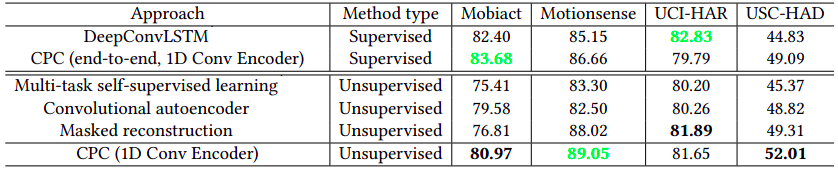
\includegraphics[width=1\textwidth]{Images/Chapter2/har-cpc-results.png}
\label{tab:har-cpc-results}
\end{table}

پس از اتمام مرحله‌ی پیش‌آموزش، کدگذار آموزش‌دیده با وزن‌های تثبیت‌شده برای استخراج ویژگی به یک مدل دسته‌بندی کاملاً متصل منتقل می‌شود تا آموزش نظارت‌شده انجام شود. همان‌طور که در جدول \ref{tab:har-cpc-results} مشاهده می‌شود، عملکرد این روش در بیشتر معیارها قابل قبول است و در برخی موارد حتی از مدل‌های کاملاً نظارت‌شده پیشی گرفته است.

\subsubsection{شناسایی فعالیت مبتنی بر روش \lr{SimCLR}}

روش \lr{SimCLR}\cite{chen2020simple} که پیش‌تر در بخش \ref{sec:simclr} معرفی شد، یکی از چارچوب‌های مطرح در یادگیری خودنظارتی مبتنی بر یادگیری تباینی است؛ اما این روش در اصل برای داده‌های تصویری ارائه شده و برای استفاده بر روی داده‌های حسگر نیازمند تغییرات و انطباق‌هایی است.

خارتدینف و همکاران\cite{khaertdinov2021contrastive} چارچوبی با عنوان \lr{CSSHAR}\LTRfootnote{Contrastive Self-Supervised Human Activity Recognition} ارائه دادند که نسخه‌ی سازگارشده‌ی \lr{SimCLR} برای شناسایی فعالیت انسان با داده‌های حسگر است. در این رویکرد، به‌جای شبکه‌های پیچشی، از یک معماری مبتنی بر مبدل (\lr{Transformer}) برای استخراج ویژگی استفاده شده است. همچنین به دلیل ماهیت متفاوت سیگنال‌های زمانی نسبت به تصاویر، مجموعه‌ای از داده‌افزایی‌های اختصاصی برای حسگرها طراحی شده که شامل موارد زیر است:

\begin{itemize}
\item \textbf{افزودن نویز:} اضافه‌کردن نویز گوسی تصادفی به سیگنال.
\item \textbf{مقیاس‌گذاری\LTRfootnote{Scaling}:} ضرب دامنه‌ی سیگنال در ضریب تصادفی از یک توزیع گوسی.
\item \textbf{چرخاندن:} معکوس‌کردن علامت نمونه‌های انتخاب‌شده به‌صورت تصادفی.
\item \textbf{جایگشت\LTRfootnote{Permutation}:} تقسیم سیگنال به چند بخش و جابه‌جایی تصادفی مقادیر در این بخش‌ها.
\end{itemize}

بسته به ویژگی‌های مجموعه‌داده، ممکن است همه یا تنها تعدادی از این تبدیلات به‌کار گرفته شوند که این انتخاب به‌صورت تجربی و با آزمون و خطا انجام می‌شود. پس از ایجاد نماهای مختلف از هر نمونه، آن‌ها به یک شبکه‌ی نگاشت (\lr{Projection Head}) وارد می‌شوند و تابع هزینه‌ی تباینی \lr{NT-Xent} برای یادگیری بازنمایی‌ها به‌کار می‌رود. در مرحله‌ی تنظیم دقیق، شبکه‌ی نگاشت حذف‌شده و یک دسته‌بند کاملاً متصل جایگزین آن می‌گردد. در این مرحله، وزن‌های کدگذار مبتنی بر مبدل ثابت نگه داشته می‌شوند تا سرعت آموزش افزایش یابد.

\begin{table}[htbp]
\centering
\caption{نتایج روش \lr{CSSHAR}}
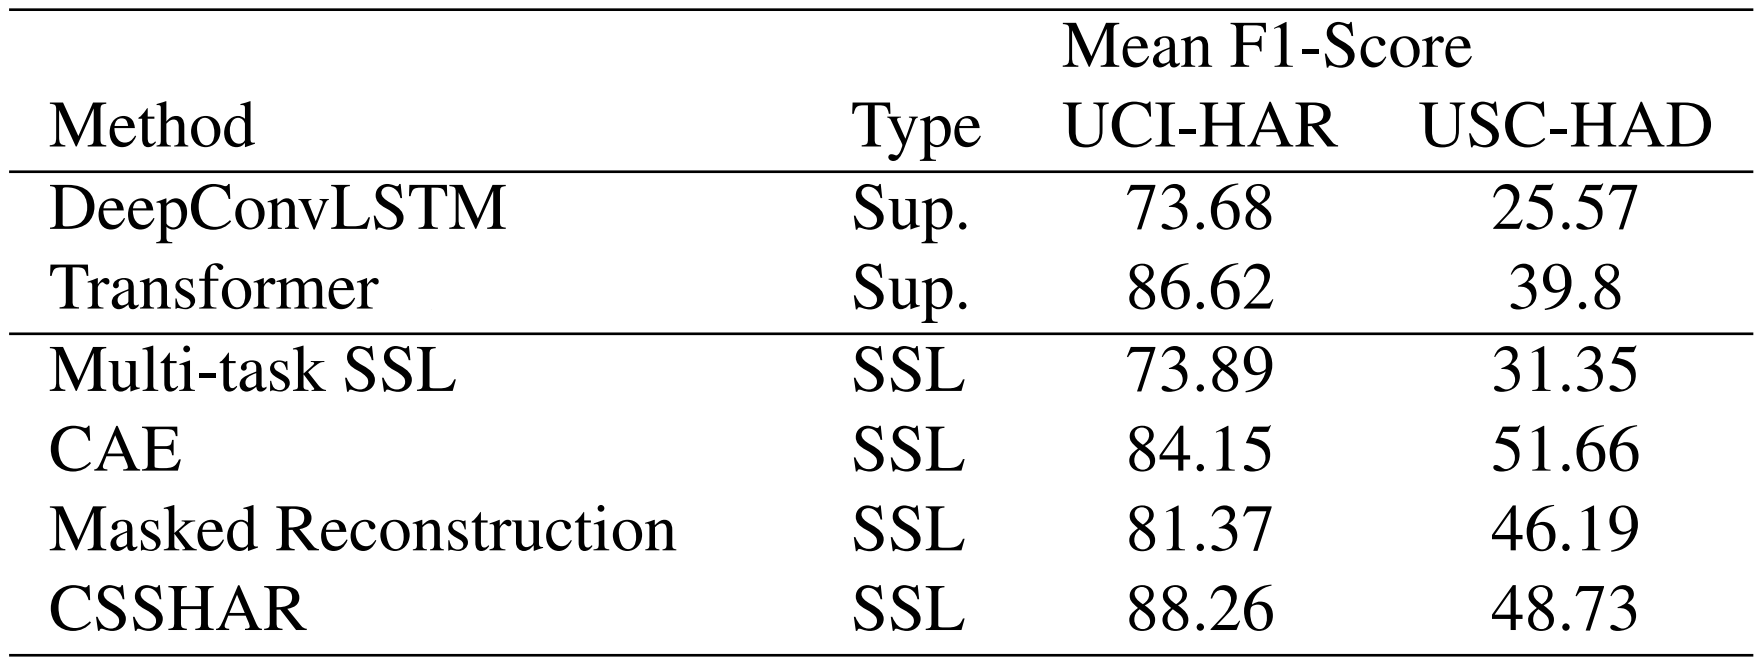
\includegraphics[width=0.75\textwidth]{Images/Chapter2/csshar-results.png}
\label{tab:csshar-results}
\end{table}

همان‌طور که در جدول \ref{tab:csshar-results} مشاهده می‌شود، ترکیب سازوکار یادگیری تباینی \lr{SimCLR} با توانایی مبدل در مدل‌سازی وابستگی‌های طولانی‌مدت سیگنال، به بهبود قابل‌توجه دقت در شناسایی فعالیت منجر شده است. این روش به‌ویژه در شرایطی که داده‌های برچسب‌خورده محدود هستند، عملکردی رقابتی یا حتی برتر نسبت به مدل‌های نظارت‌شده نشان داده است.

\subsubsection{شناسایی فعالیت مبتنی بر یادگیری مشارکتی}

جین و همکاران \cite{jain2022collossl} یک چارچوب یادگیری خودنظارتی نوین و مشارکتی\LTRfootnote{Collaborative} تحت عنوان \lr{ColloSSL} را برای پیش‌آموزش مدل‌های بازشناسی فعالیت انسان ارائه دادند. این روش برای محیط‌هایی طراحی شده است که در آن چندین حسگر به‌طور همزمان داده‌های مربوط به یک فعالیت را ثبت می‌کنند. این محیط، یک سیستم چند دستگاهی همگام با زمان (\lr{TSMDS}\LTRfootnote{Time-Synchronous Multi-Device System}) نامیده می‌شود که در آن، داده‌های ثبت‌شده توسط حسگرهای مختلف کاملا همگام هستند.

ایده‌ی اصلی \lr{ColloSSL} این است که به‌جای تولید داده‌های افزوده به‌صورت مصنوعی (مانند افزودن نویز یا دوران)، از داده‌های حسگرهای مختلف به‌عنوان تبدیل‌های طبیعی \LTRfootnote{Natural Transformations} از یکدیگر استفاده شود. به عبارت دیگر، داده‌ی ثبت‌شده توسط حسگر روی مچ دست و حسگر روی قفسه‌ی سینه، دو «نما» یا «دیدگاه» متفاوت از یک فعالیت یکسان (مثلا راه‌رفتن) هستند. هدف یادگیری تباینی در این روش، نزدیک کردن بازنمایی این نماهای مختلف از یک فعالیت و دورکردن آن‌ها از بازنمایی فعالیت‌های دیگر است.

\begin{figure}[t]
\centering
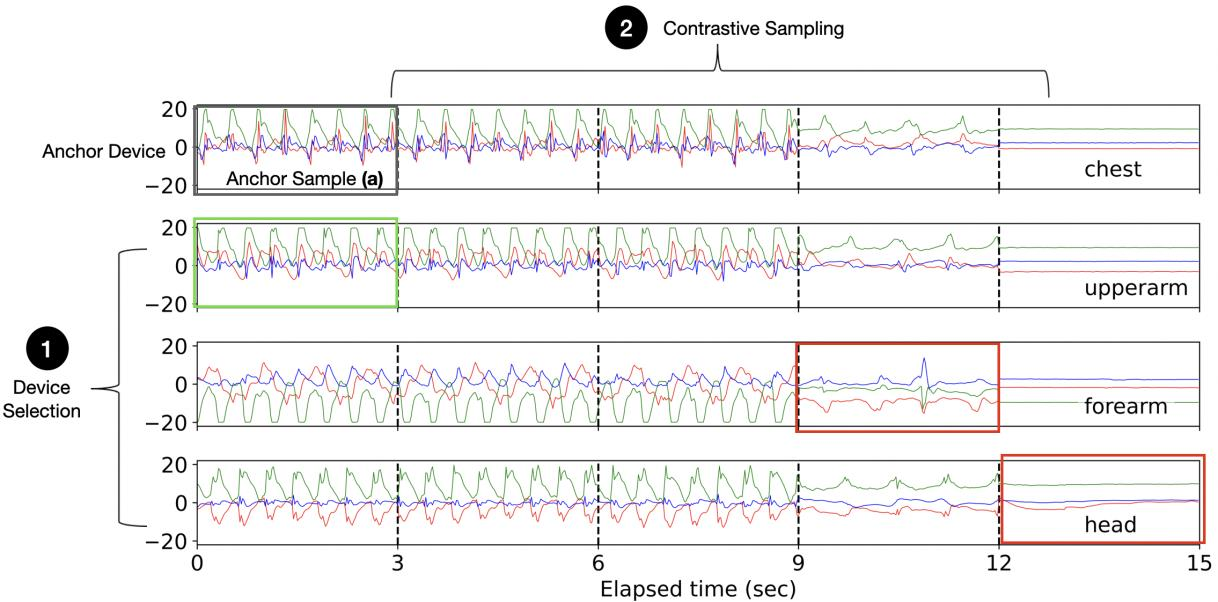
\includegraphics[width=1\textwidth]{Images/Chapter2/collossl.png}
\caption{انتخاب حسگرهای مثبت و منفی در \lr{ColloSSL}}

\label{fig:collossl}

\end{figure}

برای مثال، همانطور که در شکل \ref{fig:collossl} نمایش داده شده است، فرض کنید می‌خواهیم مدل را با محوریت داده‌های حسگر قفسه سینه پیش‌آموزش دهیم. در این حالت، این حسگر به‌عنوان دستگاه محوری \LTRfootnote{Anchor Device} انتخاب می‌شود. سپس، نمونه‌های داده از این دستگاه با نمونه‌های سایر دستگاه‌ها مقایسه می‌شوند. فرایند کلی یادگیری در این مقاله به‌صورت زیر است:

\begin{enumerate}
\item ابتدا، یک استخراج‌کننده‌ی ویژگی (در این مقاله، یک شبکه‌ی پیچشی یک‌بعدی با سه لایه) با وزن‌های تصادفی مقداردهی اولیه می‌شود.
\item یک دسته‌ی تصادفی از داده‌ها انتخاب می‌شود. این دسته شامل پنجره‌های زمانی (مثلا به طول ۳ ثانیه) از تمام حسگرها است. نکته‌ی کلیدی این است که این پنجره‌ها از نظر زمانی با یکدیگر همگام هستند.
\item برای شروع یادگیری تباینی، یک نمونه از یک دستگاه خاص (مثلاً قفسه سینه) به‌عنوان نمونه‌ی محوری \LTRfootnote{Anchor Sample} انتخاب می‌شود.
\item نمونه‌های زمانی متناظر با نمونه‌ی محوری از سایر دستگاه‌ها (مانند مچ، ران و غیره) به‌عنوان نمونه‌های مثبت در نظر گرفته می‌شوند. این نمونه‌ها دیدگاه‌های متفاوتی از همان فعالیت در همان لحظه هستند.
\item تمام نمونه‌های دیگر در آن دسته (که متعلق به پنجره‌های زمانی دیگری هستند) به‌عنوان نمونه‌های منفی انتخاب می‌شوند.
\item تمام این نمونه‌ها (محوری، مثبت و منفی) به استخراج‌کننده‌ی ویژگی داده می‌شوند تا بازنمایی نهفته‌ی آن‌ها استخراج شود. سپس با استفاده از یک تابع زیان تباینی، مدل آموزش داده می‌شود. هدف این تابع زیان، به حداکثر رساندن شباهت بین بازنمایی نمونه‌ی محوری و نمونه‌های مثبت، و به حداقل رساندن شباهت آن با نمونه‌های منفی است.
\item مراحل ۳ تا ۶ برای تمام نمونه‌های موجود در دسته تکرار می‌شوند تا مدل به‌طور کامل یاد بگیرد که چگونه بازنمایی‌های معناداری از فعالیت‌ها استخراج کند. این فرایند با انتخاب دسته‌های جدید ادامه می‌یابد.
\end{enumerate}

در نهایت، مزیت کلیدی چارچوب \lr{ColloSSL} در تعریف هوشمندانه‌ی وظیفه‌ی پیش‌آموزشی آن نهفته است. این روش با بهره‌گیری از داده‌های همگامِ حسگرهای مختلف، یک سیگنال نظارتی غنی و طبیعی را بدون نیاز به هیچ‌گونه برچسب‌گذاری انسانی یا افزونه‌سازی مصنوعی ایجاد می‌کند. در نتیجه، استخراج‌کننده‌ی ویژگی حاصل، بازنمایی‌هایی عمیق و پایدار از فعالیت‌های انسانی را فرا می‌گیرد که می‌تواند به‌عنوان یک پایه‌ی قدرتمند برای بهبود عملکرد و کاهش نیاز به داده‌های برچسب‌دار در مدل‌های دسته‌بندی نهایی عمل کند.

\section{جمع‌بندی}

در این فصل، ادبیات موضوع و کارهای پیشین در حوزه‌ی شناسایی فعالیت انسان و یادگیری خودنظارتی مورد بررسی قرار گرفت. ابتدا به بررسی روش‌های شناسایی فعالیت انسان پرداختیم. سپس چالش اصلی روش‌های یادگیری عمیق، یعنی نیاز به حجم بالای داده‌های برچسب‌دار، تشریح شد. در ادامه، یادگیری خودنظارتی به‌عنوان یک راهکار موثر برای غلبه بر این محدودیت معرفی گردید که با تعریف وظایف پوششی بر روی داده‌های خام، به یادگیری بازنمایی‌های غنی می‌پردازد. در نهایت، با مرور پژوهش‌های ترکیبی در این دو حوزه، نشان داده شد که اقتباس روش‌های خودنظارتی، به‌ویژه رویکردهای تباینی، برای داده‌های حسگری به نتایج امیدوارکننده‌ای منجر شده و می‌تواند عملکردی قابل مقایسه با روش‌های کاملاً نظارت‌شده، با نیاز به مراتب کمتری به داده‌های برچسب‌دار، ارائه دهد.

\chapter{روش پیشنهادی}
\clearpage

در این فصل، به تشریح کامل روش پیشنهادی می‌پردازیم. نخست، به‌عنوان پیش‌نیاز، به تعریف تبدیل موجک\LTRfootnote{Wavelet Transform} و
اسکالوگرام\LTRfootnote{Scalogram}
خواهیم پرداخت. سپس، روش پایه و معماری آن را به تفصیل مورد بررسی قرار می‌دهیم. در نهایت، با تحلیل این معماری، زمینه‌های مستعد بهبود در آن شناسایی شده و سپس نوآوری‌های ارائه شده در این پژوهش که برای رفع این چالش‌ها طراحی شده‌اند، به تفصیل تشریح خواهند شد.

\section{تبدیل موجک}

تبدیل موجک یکی از ابزارهای قدرتمند در پردازش سیگنال است که برای تحلیل سیگنال‌ها در هر دو حوزه‌ی زمان و فرکانس به صورت همزمان به کار می‌رود. این ویژگی، تبدیل موجک را از ابزارهای کلاسیک مانند
تبدیل فوریه\LTRfootnote{Fourier Transform}
متمایز می‌سازد. تبدیل فوریه، سیگنال را به مولفه‌های فرکانسی تشکیل‌دهنده‌ی آن از طریق دو طیف دامنه و فاز تجزیه می‌کند. طیف دامنه نشان می‌دهد که هر مولفه‌ی فرکانسی با چه شدتی در کل سیگنال حضور دارد، اما اطلاعاتی در مورد زمان وقوع آن ارائه نمی‌دهد. اگرچه طیف فاز به صورت غیرمستقیم حاوی اطلاعات زمانی است، اما تفسیر آن برای محلی‌سازی رویدادها در زمان بسیار دشوار و غیرمستقیم است. به عبارت دیگر، تبدیل فوریه در نمایش همزمان رویدادها در حوزه‌ی زمان و فرکانس دارای محدودیت است. در مقابل، تبدیل موجک با استفاده از توابعی به نام
موجک مادر\LTRfootnote{Mother Wavelet}
که در زمان و فرکانس محدود هستند، این محدودیت را برطرف می‌سازد.

ایده‌ی اصلی در تبدیل موجک، مقایسه‌ی سیگنال با نسخه‌های جابه‌جا شده و مقیاس‌گذاری شده از یک موجک مادر است. جابه‌جایی به منظور محلی‌سازی تحلیل در زمان و مقیاس‌گذاری به منظور محلی‌سازی تحلیل در فرکانس انجام می‌شود. مقیاس‌های کوچک (فشرده‌سازی موجک) متناظر با فرکانس‌های بالا و مقیاس‌های بزرگ (کشیده‌سازی موجک) متناظر با فرکانس‌های پایین هستند.

تبدیل موجک به دو دسته‌ی اصلی گسسته (\lr{DWT\LTRfootnote{Discrete Wavelet Transform}}
و پیوسته (\lr{CWT\LTRfootnote{Continuous Wavelet Transform}})
تقسیم می‌شوند که در این پژوهش از تبدیل موجک پیوسته استفاده کرده‌ایم.

تبدیل موجک یک سیگنال زمانی $x(t)$
به فرم زیر تعریف می‌گردد:
\begin{equation}
    \label{eq:wavelet-transform}
    CWT(a, b) = \int_{-\infty}^{\infty} x(t) \psi_{a,b}(t) dt
\end{equation}
که در این معادله، $\psi_{a,b}(t)$
موجک دختر\LTRfootnote{Daughter Wavelet}
نامیده می‌شود که نسخه‌ی مقیاس‌گذاری و جابه‌جا شده است و به فرم زیر تعریف می‌گردد:
\begin{equation}
    \label{eq:daughter-wavelet}
    \psi_{a,b}(t) = \frac{1}{\sqrt{|a|}} \psi \left( \frac{t - b}{a} \right)
\end{equation}
در این رابطه، پارامتر $a$ مقیاس است
که با فرکانس رابطه‌ی معکوس دارد. پارامتر $b$
بیانگر میزان جابه‌جایی در محور زمان است و ضریب
$\frac{1}{\sqrt{|a|}}$
برای نرمال‌سازی انرژی موجک به‌کار می‌رود.
$\psi(t)$
نیز یک تابع ریاضی است که باید دارای میانگین صفر و انرژی محدود در تمام دامنه باشد. برای مثال موجک مورلت\LTRfootnote{Morlet Wavelet}
که فرمول آن به فرم رابطه‌ی \ref{eq:morlet-wavelet}
می‌باشد، یک موجک بسیار کاربردی در حوزه‌ی سیگنال‌های دنیای واقعی، به‌خصوص سیگنال‌های مربوط به فعالیت انسان می‌باشد. چرا که در این سیگنال‌ها، معمولا نوسانات و فرکانس‌های غیر ایستا داریم که به سرعت محو می‌شوند و موجک مورلت به‌دلیل دارا بودن $e^{\frac{-t^2}{2}}$
که به آن اثر محوشدگی را می‌دهد، برای این‌گونه سیگنال‌ها بسیار مناسب است.
\begin{equation}
    \label{eq:morlet-wavelet}
    \psi(t) = \frac{\cos(\omega_0 t) e^{-\frac{t^2}{2}}}{\pi^{\frac{1}{4}}}
\end{equation}
خروجی \lr{CWT}
مجموعه‌ای از ضرایب است که میزان شباهت سیگنال $x(t)$
را با موجک با مقیاس $a$ و زمان $b$
نشان می‌دهد. این ضرایب یک نمایش دوبعدی از سیگنال یک بعدی اولیه ارائه می‌دهند که به آن اسکالوگرام می‌گویند. در یک اسکالوگرام محور افقی بیانگر میزان جابه‌جایی یا همان $b$ و
محور عمودی بیانگر مقیاس‌ها می‌باشد. یک نمونه اسکالوگرام در شکل \ref{fig:wavelet-plot} قابل مشاهده می‌باشد.
\begin{figure}[htb!]
\centering
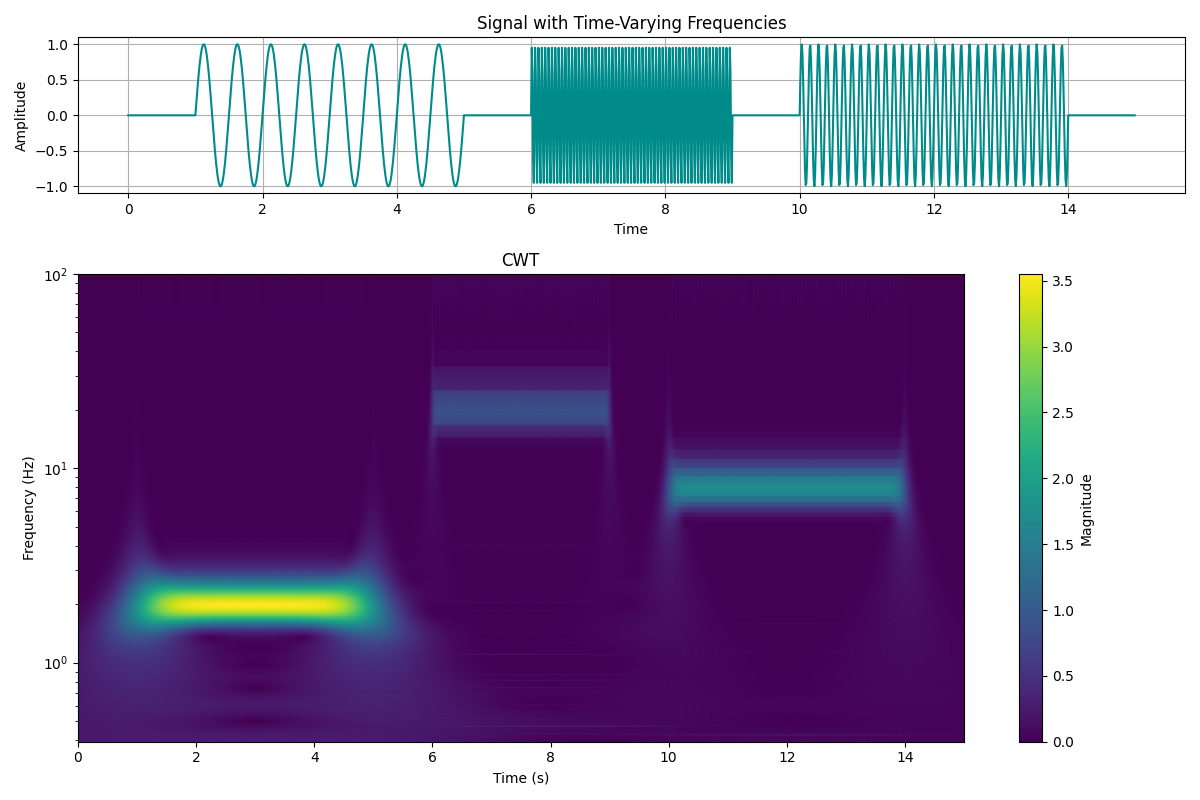
\includegraphics[width=1\textwidth]{Images/Chapter3/wavelet-plot.png}
\caption{نمونه اسکالوگرام برای یک موج متغیر در زمان}
\label{fig:wavelet-plot}
\end{figure}

\section{روش پایه}

معماری کلی پیش‌آموزش خودنظارتی روش پیشنهادی در شکل \ref{fig:proposed-method-pretraining}
قابل مشاهده است. این معماری توسط طاقانکی و همکاران\cite{taghanaki2023self}
برای پیش‌آموزش یک مدل جهت استخراج بازنمایی‌های مفید از روی داده‌های سیگنال مربوط به شناسایی فعالیت انسان ارائه شد. این معماری با این فرضیه طراحی شده است که اطلاعات مفید مربوط به فعالیت در هر دو حوزه زمان و فرکانس نهفته است. به همین منظور، از دو مسیر پردازشی مجزا برای استخراج ویژگی از سیگنال ورودی استفاده می‌شود. یک کدگذار سیگنال که وظیفه‌ی آن پردازش داده‌های خام سیگنال می‌باشد و یک کدگذار اسکالوگرام که وظیفه‌ی آن پردازش اسکالوگرام‌های حاصل از تبدیل موجک
بر روی داده‌های خام سیگنال می‌باشد.

\begin{figure}[ht]
\centering
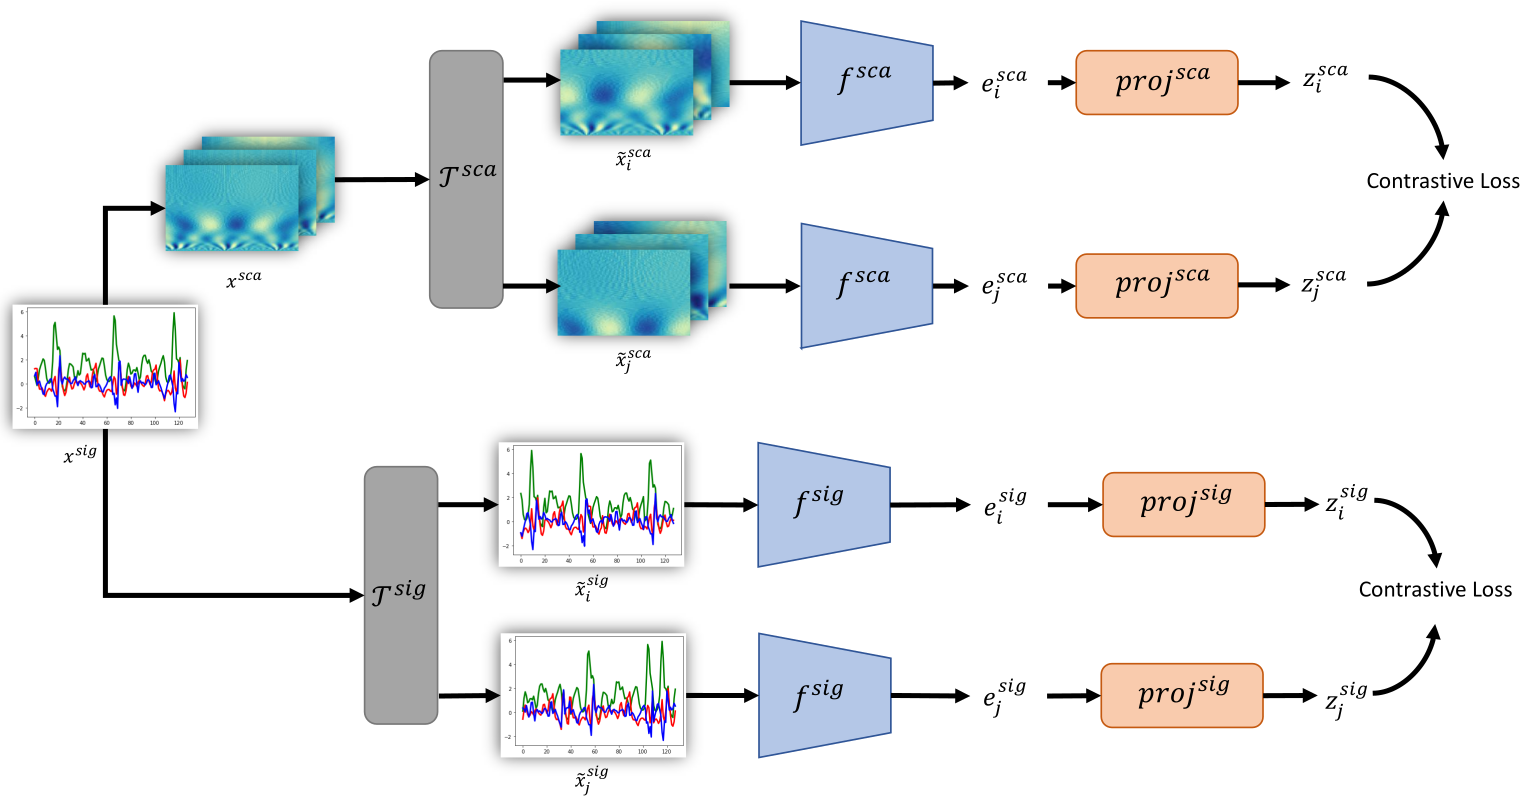
\includegraphics[width=1\textwidth]{Images/Chapter3/proposed-method-pretraining.png}
\caption{معماری کلی پیش‌آموزش در روش پیشنهادی}
\label{fig:proposed-method-pretraining}
\end{figure}

در ادامه به بررسی جزئیات مربوط به هر دو مسیر آموزش کدگذار می‌پردازیم.

\subsection{کدگذار سیگنال}

این بخش از معماری وظیفه‌ی یادگیری از روی داده‌های خام سیگنال در حوزه‌ی زمان را بر عهده دارد. برای آموزش این بخش، از چارچوب یادگیری تباینی
\lr{SimCLR}
که در فصل قبل درباره‌ی جزئیات آن توضیح دادیم استفاده شده است. کدگذار سیگنال یا
$\mathcal{H}_{sig}$
از یک شبکه عصبی شامل ۳ لایه پیچشی یک بعدی تشکیل شده است. سپس خروجی $\mathcal{H}_{sig}$
به یک شبکه نگاشت داده می‌شود و در نهایت بر روی خروجی شبکه نگاشت تابع هزینه تباینی \lr{NT-Xent} به‌فرم معادله \ref{eq:simclr-loss}
اعمال می‌شود.
پیاده‌سازی چارچوب \lr{SimCLR} مستلزم تعریف مجموعه‌ای از تبدیلات داده‌افزایی است. در این مسیر، تبدیلات زیر برای اعمال بر روی سیگنال خام زمانی به کار گرفته شده‌اند:
\begin{itemize}
    \item\textbf{نویز:} یک نویز تصادفی گوسی با میانگین صفر و انحراف معیار $0.1$ اعمال می‌شود.
    \item\textbf{مقیاس‌دهی\LTRfootnote{Scale}:}
    یک مقدار تصادفی با میانگین $1$ و انحراف معیار $0.2$ در سیگنال ضرب می‌شود.
    \item\textbf{معکوس‌سازی زمانی\LTRfootnote{Time Flip}:}
    با یک احتمال ثابت، پنجره سیگنال ورودی نسبت به زمان معکوس می‌گردد. ایده‌ی پشت این تبدیل این است که یک فعالیت ممکن است در جهت برعکس انجام شود.
    \item\textbf{بر زدن کانال‌ها\LTRfootnote{Channel Shuffle}:}
    با یک احتمال ثابت، کانال‌های سیگنال ورودی به‌صورت تصادفی با یکدیگر جابه‌جا می‌شوند. ایده‌ی پشت این تبدیل این است که ممکن است حسگر در یک جهتی عمود بر جهت استاندارد قرار گرفته باشد. مثلا جهت قرار گرفتن تلفن همراه هوشمند در جیب شخص. نکته‌ی مهم در رابطه با این تبدیل این است که فقط کانال‌های مربوط به هر دستگاه باید با یکدیگر جابه‌جا شوند. مثلا اگر کانال‌های اول تا سوم برای شتاب‌سنج و کانال‌های چهارم تا ششم برای ژیروسکوپ باشند، کانال‌های اول تا سوم با یکدیگر و کانال‌های چهارم تا ششم نیز با یکدیگر جابه‌جا می‌شوند.
    \item\textbf{جایگشت:} سیگنال ورودی به قطعاتی تقسیم می‌شود و این قطعات با یکدیگر جابه‌جا می‌شوند. ایده‌ی پشت این تبدیل این است که ممکن است ترتیب بخش‌های مربوط به انجام یک فعالیت تغییر کنند.
    \item\textbf{چرخش:}
    سیگنال ورودی حول یک محور تصادفی و به میزان درجه‌ی تصادفی چرخش داده می‌شود. در واقع چرخش، حالت کلی‌تر از بر زدن کانال‌ها می‌باشد.
\end{itemize}

انتخاب تبدیلات بهینه و ترکیب آن‌ها، فرایندی تجربی و وابسته به مشخصات هر مجموعه داده است. اما به‌طور کلی تبدیلات نه باید به‌قدری سخت و شدیدا تصادفی باشند که مدل کلا نتواند الگویی کشف کند، و نه باید به‌قدری ساده باشند که مدل به سراغ کشف بازنمایی‌های مفید و جامع نرود.

\subsection{کدگذار اسکالوگرام}

این بخش از معماری وظیفه‌ی یادگیری از روی اسکالوگرام‌های حاصل از اعمال تبدیل موجک بر روی سیگنال‌ها را بر عهده دارد. همانند کدگذار سیگنال، در کدگذار اسکالوگرام نیز از روش \lr{SimCLR}
برای آموزش مدل استفاده شده است. کدگذار اسکالوگرام یا
$\mathcal{H}_{sca}$
از یک شبکه عصبی شامل ۳ لایه پیچشی دو بعدی تشکیل شده است. قبل از این که یک پنجره‌ی چندکاناله از داده‌ها وارد این شبکه شوند، بر روی آن‌ها تبدیل موجک اعمال می‌شود و با اسکالوگرام حاصل می‌توان مانند یک تصویر رفتار کرد.

روش‌های داده‌افزایی به‌کار رفته در کدگذار اسکالوگرام نیز به شرح زیر می‌باشند:
\begin{itemize}
    \item\textbf{اعوجاج رنگ تصادفی\LTRfootnote{Random Color Distortion}:}
    در این تبدیل، هر کانال مربوط به هر حسگر را یک رنگ در نظر می‌گیریم و رنگ آن را به‌صورت تصادفی دچار اعوجاج و تغییرات می‌کنیم. مثلا شدت رنگ‌ها را افزایش می‌دهیم و یا آن را به فرم سیاه و سفید درمی‌آوریم.
    \item\textbf{برش تصادفی:}
    به‌صورت تصادفی اسکالوگرام‌ها را برش می‌زنیم.
    \item\textbf{معکوس‌سازی زمانی:}
    اسکالوگرام‌ها را به‌صورت افقی معکوس می‌کنیم.
\end{itemize}

\subsection{تنظیم دقیق مدل}

پس از این که هر دو کدگذار فرایند پیش‌آموزش را پشت سر گذاشتند، مانند روش \lr{SimCLR}
شبکه نگاشت کنار گذاشته می‌شود و به‌جای آن یک شبکه متشکل از دو لایه‌ی تماما متصل برای دسته‌بندی قرار داده می‌شوند. این کار را برای هر دو کدگذار به‌صورت مستقل انجام می‌دهیم. سپس وزن‌های لایه‌های پیچشی هر دو کدگذار تثبیت می‌شوند. این عمل دو هدف اصلی را دنبال می‌کند: اولا، از بیش‌برازش مدل بر روی داده‌های برچسب‌دار که معمولا حجم کمتری دارند جلوگیری می‌کند و ثانیا، بازنمایی‌های کلی و مفیدی که در مرحله پیش‌آموزش یاد گرفته شده‌اند، حفظ می‌شوند. در نهایت دو دسته‌بندی کننده خواهیم داشت که هر یک جداگانه آموزش دیده‌اند؛ یکی بر روی داده‌های خام و دیگری بر روی اسکالوگرام‌ها. در نهایت برای به‌دست آمدن دسته‌بند نهایی، بایستی خروجی دو دسته‌بند با یکدیگر ادغام شوند. در این روش، از راهبرد
ادغام در سطح امتیاز\LTRfootnote{Score-Level Fusion}
که به آن
ادغام دیرهنگام\LTRfootnote{Late Fusion}
نیز گفته می‌شود، استفاده شده است. در این روش، بردارهای احتمال خروجی از هر دو دسته‌بند (به عنوان مثال از طریق میانگین‌گیری) با یکدیگر ترکیب شده و سپس دسته‌ی نهایی بر اساس بیشترین امتیاز در بردار حاصل انتخاب می‌گردد.

\section{نوآوری‌های پیشنهادی}

همان‌طور که تشریح شد، روش پایه یک چارچوب قدرتمند و منطقی برای یادگیری بازنمایی از سیگنال‌های فعالیت انسان ارائه می‌دهد. با این وجود، تحلیل دقیق این معماری نشان می‌دهد که چندین مولفه کلیدی در آن، ظرفیت بهبود و بهینه‌سازی را دارا هستند. در این پژوهش، دو حوزه اصلی برای ارتقای مدل پایه شناسایی و مورد هدف قرار گرفته است:
\begin{itemize}
    \item\textbf{الگوریتم یادگیری تباینی:}
    با وجود این که چارچوب یادگیری تباینی \lr{SimCLR}
    عملکرد خوبی از خود در حوزه‌های مختلف نشان داده است، می‌توان از رویکردهای دیگر یادگیری تباینی که در دیگر حوزه‌ها عملکرد بهتری از خود نشان داده‌اند استفاده کرد.
    \item\textbf{راهبرد داده‌افزایی:}
    روش‌های داده‌افزایی اعمال‌شده بر روی اسکالوگرام‌ها مستقیما از حوزه بینایی کامپیوتر اقتباس شده‌اند و ممکن است بهترین گزینه برای داده‌های زمان-فرکانس نباشند. بنابراین، یک راهبرد داده‌افزایی جدید و متناسب با ماهیت این داده‌ها ارائه می‌شود.
\end{itemize}

\subsection{الگوریتم یادگیری تباینی \lr{SwAV}}

الگوریتم یادگیری تباینی
\textbf{تعویض انتساب‌ها میان نماها} یا به‌اختصار \lr{SwAV\LTRfootnote{Swapping Assignments between Views}}،
یک الگوریتم یادگیری تباینی مبتنی بر خوشه‌بندی می‌باشد که توسط کارون و همکاران\cite{caron2020unsupervised} ارائه شد. این الگوریتم با هدف یادگیری بازنمایی‌های بصری قدرتمند بدون نیاز به برچسب‌های انسانی طراحی شده و توانسته است فاصله‌ی عملکردی میان روش‌های خودنظارتی و نظارت‌شده را به شکل چشمگیری کاهش دهد.

ایده‌ی اصلی این الگوریتم بر یک سازوکار پیش‌بینی تعویض‌شده\LTRfootnote{Swapped Prediction}
استوار است. در این روش، به جای مقایسه‌ی مستقیم بردارهای ویژگی حاصل از نماهای مختلف یک تصویر با یکدیگر (کاری که در روش‌های متداولی مانند \lr{SimCLR} انجام می‌شود)، مدل می‌آموزد که تخصیص خوشه‌ی یک نما را از روی بردار ویژگی نمای دیگر پیش‌بینی کند. به عبارت دیگر، اگر دو نمای مختلف از یک تصویر ورودی داشته باشیم، ویژگی‌های استخراج‌شده از نمای اول باید آن‌قدر غنی و معنادار باشند که بتوان با استفاده از آن‌ها، کد خوشه‌ی مربوط به نمای دوم را پیش‌بینی کرد و بالعکس. این فرایند، مدل را وادار می‌سازد تا بازنمایی‌هایی را بیاموزد که نسبت به تبدیلات و تغییرات اعمال‌شده بر روی تصویر (مانند برش، تغییر رنگ و دوران) نامتغیر و پایدار باشند.

\begin{figure}[htb!]
\centering
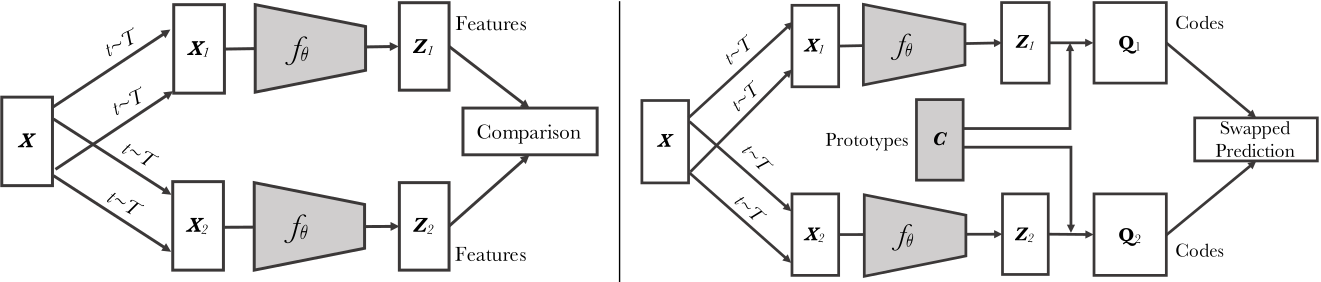
\includegraphics[width=0.8\textwidth]{Images/Chapter3/swav-comparison.png}
\caption{مقایسه‌ی الگوریتم \lr{SwAV} (سمت راست) و \lr{SimCLR} (سمت چپ)}
\label{fig:wavelet-plot}
\end{figure}

یکی از نوآوری‌های کلیدی روش \lr{SwAV}، انجام فرایند خوشه‌بندی به صورت برخط\LTRfootnote{Online}
است. در روش‌های مبتنی بر خوشه‌بندی پیشین
(مانند روش خوشه عمیق\LTRfootnote{Deep Cluster}\cite{caron2018deep})،
فرایند یادگیری به دو مرحله‌ی مجزا و غیر برخط تقسیم می‌شد: ابتدا تمام داده‌ها برای تخصیص به خوشه‌ها پردازش شده و سپس از این تخصیص‌ها به عنوان برچسب‌های کاذب برای آموزش شبکه استفاده می‌شد.  این فرایند نیازمند عبورهای چندباره از کل مجموعه داده بود و مقیاس‌پذیری الگوریتم را با چالش مواجه می‌کرد. اما در \lr{SwAV}، تخصیص خوشه‌ها تنها با استفاده از نمونه‌های موجود در هر دسته‌ی آموزشی از داده‌ها و به صورت آنی انجام می‌شود. این ویژگی باعث می‌شود که \lr{SwAV} بسیار کارآمد بوده و بتواند بر روی مجموعه‌داده‌های بسیار بزرگ نیز به راحتی آموزش ببیند.

\subsubsection{تابع هزینه پیش‌بینی تعویض‌شده}

همان‌طور که اشاره کردیم، هسته‌ی اصلی الگوریتم \lr{SwAV} بر مبنای یک تابع هزینه‌ی منحصربه‌فرد به نام «پیش‌بینی تعویض‌شده» قرار دارد. این تابع هزینه، سازگاری میان نماهای مختلف یک تصویر را نه از طریق مقایسه‌ی مستقیم ویژگی‌ها، بلکه از طریق مقایسه‌ی تخصیص خوشه‌های آن‌ها می‌سنجد.

فرض کنید برای یک تصویر ورودی، دو نمای مختلف با اعمال تبدیلات تصادفی ایجاد کرده‌ایم و پس از عبور آن‌ها از شبکه‌ی کدگذار، بردارهای ویژگی
$z_t$ و $z_s$ را به‌دست آورده‌ایم.
تابع هزینه‌ی \lr{SwAV} برای این زوج ویژگی به صورت زیر تعریف می‌شود:
\begin{equation}
    L(z_t, z_s) = \ell(z_t, q_s) + \ell(z_s, q_t)
    \label{eq:swav-loss}
\end{equation}
در این رابطه:
\begin{itemize}
    \item $z_t$ و $z_s$ بردارهای ویژگی نرمال‌شده‌ی حاصل از دو نما هستند.
    \item $q_t$ و $q_s$ کدهای خوشه یا بردارهای تخصیص نرم\LTRfootnote{Soft Assignment Vectors} مربوط به هر یک از این ویژگی‌ها می‌باشند. این کدها که در عمل یک توزیع احتمال هستند، نشان می‌دهند که هر ویژگی تا چه حد به هر یک از خوشه‌های موجود در مدل تعلق دارد.
    \item $\ell(z,q)$ تابعی است که میزان اختلاف میان یک توزیع پیش‌بینی‌شده (که از $z$ حاصل می‌شود) و یک کد هدف ($q$) را اندازه‌گیری می‌کند.
\end{itemize}
فرمول \ref{eq:swav-loss} دارای دو بخش متقارن است. بخش اول، $\ell(z_t,q_s)$
مدل را وادار می‌کند تا با استفاده از ویژگی نمای اول ($z_t$) کد خوشه‌ی نمای دوم ($q_s$) را پیش‌بینی کند. بخش دوم نیز این فرایند را به‌صورت معکوس انجام می‌دهد. به همین دلیل این سازوکار، پیش‌بینی تعویض‌شده نام گرفته است.

تابع $\ell(z,q)$ در عمل یک تابع هزینه آنتروپی متقاطع است که اختلاف میان دو توزیع احتمال را می‌سنجد:
\begin{itemize}
    \item\textbf{توزیع پیش‌بینی شده \lr{p}:} یک توزیع احتمال که از بردار ویژگی $z$ به دست می‌آید و نشان‌دهنده‌ی پیش‌بینی مدل برای تخصیص آن ویژگی به خوشه‌هاست.
    \item\textbf{کد هدف \lr{q}:} یک توزیع احتمال که به عنوان برچسب نرم عمل می‌کند و از قبل برای نمای دیگر محاسبه شده است.
\end{itemize}

\noindent\textbf{محاسبه توزیع پیش‌بینی‌شده (\lr{p}): از ویژگی به احتمال}

توزیع $p$،
پیش‌بینی مدل از میزان تعلق یک بردار ویژگی $z$
به هر یک از $K$ خوشه موجود را نشان می‌دهد. مراکز خوشه‌ها را با بردارهایی تحت عنوان پیش‌نمونه\LTRfootnote{Prototype} نشان می‌دهیم که این مراکز خوشه‌ها مجموعه‌ای از بردارهای قابل یادگیری $C=\{c_1,...,c_k\}$
در فضای ویژگی هستند.

فرایند تبدیل بردار ویژگی 
$z$
به توزیع احتمال 
$p$
در دو مرحله‌ی اصلی انجام می‌شود: ابتدا محاسبه‌ی امتیازات شباهت و سپس تبدیل این امتیازات به یک توزیع احتمال معتبر.

در گام نخست، مدل میزان شباهت میان بردار ویژگی
$z_t$
و هر یک از 
$K$
بردار مرکز خوشه را محاسبه می‌کند. این شباهت از طریق ضرب داخلی میان بردار ویژگی و هر بردار $c_k$
به دست می‌آید. نتیجه‌ی این عملیات، یک بردار با 
$K$
درایه است که هر درایه‌ی آن، که هر درایه‌ی آن، امتیاز شباهت خام یا \lr{Logit} نامیده می‌شود و نشان‌دهنده‌ی میزان تطابق ویژگی با آن بردار مرکز خوشه خاص است.

امتیازات خام به دست آمده، مقادیری نامحدود هستند و مجموع آن‌ها لزوما برابر با یک نیست. برای تبدیل آن‌ها به یک توزیع احتمال معتبر، از تابع سافت‌مکس\LTRfootnote{Softmax} استفاده می‌شود. این تابع، هر امتیاز را به یک مقدار در بازه‌ی $(0, 1)$ نگاشت کرده و تضمین می‌کند که مجموع تمام احتمالات برابر با یک شود. در این فرایند، از یک پارامتر دما $\tau$ نیز برای کنترل تیزی یا همواری توزیع خروجی استفاده می‌شود. دمای پایین‌تر منجر به توزیعی تیزتر (با قطعیت بیشتر) و دمای بالاتر منجر به توزیعی هموارتر می‌گردد. بنابراین، احتمال تعلق ویژگی 
$z_t$
به خوشه 
$k$ام که با
$p_t^{(k)}$
نمایش داده می‌شود، از طریق فرمول زیر محاسبه می‌گردد:
\begin{equation}
p_t^{(k)} = \frac{\exp(\frac{1}{\tau} z_t^\top c_k)}{\sum_{k'=1}^{K} \exp(\frac{1}{\tau} z_t^\top c_{k'})}
\label{eq:swav-p-calculation}
\end{equation}
در این فرمول،
$z_t^kc_k$
همان ضرب داخلی میان بردار ویژگی و بردار مرکز خوشه $k$ام است.
مخرج کسر نیز مجموع مقادیر صورت کسر برای تمام 
$K$
مرکز خوشه است که برای نرمال‌سازی به کار می‌رود. این توزیع
$p_t$
همان پیش‌بینی مدل برای بردار ویژگی $z_t$ است که در تابع هزینه‌ی آنتروپی متقاطع با کد هدف
$q_s$
مقایسه خواهد شد.

\vspace{0.5em}
\noindent\textbf{محاسبه کدهای هدف \lr{q}: تخصیص بهینه خوشه‌ها}

اکنون به بخش پیچیده‌تر محاسبه‌ی تابع هزینه، یعنی نحوه‌ی تعیین کدهای هدف 
$q$
می‌رسیم. برخلاف توزیع پیش‌بینی‌شده 
$p$
که به سادگی از خروجی شبکه به دست می‌آمد، محاسبه‌ی 
$q$
نیازمند یک سازوکار ویژه برای جلوگیری از یک مشکل اساسی است.

یک چالش مهم در روش‌های مبتنی بر خوشه‌بندی، پدیده‌ای است که با عناوینی چون پاسخ بدیهی\LTRfootnote{Trivial Solution}
یا فروپاشی مدل\LTRfootnote{Model Collapse}
شناخته می‌شود. این مشکل زمانی رخ می‌دهد که مدل یک راه‌حل ساده و بی‌ارزش برای کمینه کردن تابع هزینه پیدا کند. در مسئله‌ی ما، مدل می‌تواند یاد بگیرد که تمام بردارهای ویژگی را به یک خوشه‌ی یکسان تخصیص دهد. در این حالت، اگرچه تابع هزینه به سرعت کمینه می‌شود، اما بازنمایی‌های آموخته‌شده هیچ اطلاعات مفیدی در مورد تمایز میان تصاویر مختلف نخواهند داشت و عملا بی‌ارزش خواهند بود.

برای مقابله با این پدیده، الگوریتم \lr{SwAV}
یک قید افراز برابر\LTRfootnote{Equipartition Constraint}
را بر روی فرایند تخصیص خوشه‌ها اعمال می‌کند. هدف این قید، وادار کردن مدل به استفاده از تمام ظرفیت بردارهای مربوط به مراکز خوشه‌ها است. این قید تضمین می‌کند که نمونه‌های موجود در یک دسته آموزشی از داده‌ها، تا حد امکان به صورت یکنواخت و برابر میان تمام 
$K$
خوشه موجود توزیع شوند.

مسئله‌ی تخصیص بهینه‌ی مجموعه‌ای از منابع (ویژگی‌های مربوط به داده‌ها) به مجموعه‌ای از مقاصد (خوشه‌ها) تحت یک سری قیود، یک مسئله‌ی کلاسیک در ریاضیات و علوم کامپیوتر است که با عنوان مسئله‌ی انتقال بهینه\LTRfootnote{Optimal Transport}
شناخته می‌شود. الگوریتم \lr{SwAV} از این چارچوب قدرتمند ریاضی برای محاسبه‌ی ماتریس تخصیص خوشه‌ها
($Q$) استفاده می‌کند.

برای درک بهتر، می‌توان این مسئله را با یک مثال ملموس توصیف کرد. فرض کنید 
$B$
 انبار (بردارهای ویژگی) و 
$K$
 فروشگاه (خوشه‌ها) داریم. هدف، طراحی یک برنامه‌ی حمل و نقل
 (ماتریس $Q$)
 است که کالاها را از انبارها به فروشگاه‌ها به بهینه‌ترین شکل ممکن ارسال کند. بهینه بودن در اینجا به دو معناست: اولا، مجموع شباهت میان انبارها و فروشگاه‌های متناظرشان بیشینه شود و ثانيا، قیود توزیع عادلانه (قید افراز برابر) که در بخش قبل به آن اشاره شد، رعایت گردد.

 به زبان ریاضی، این مسئله به صورت یافتن ماتریس $Q$ از میان مجموعه‌ی تمام ماتریس‌های معتبر 
$\mathcal{Q}$
(که در قیود افراز برابر صدق می‌کنند) تعریف می‌شود که عبارت زیر را بیشینه کند:
\begin{equation}
\max_{Q \in \mathcal{Q}} Tr(Q^\top C^\top Z) + \epsilon H(Q)
\label{eq:swav-optimal-transport}
\end{equation}
در این رابطه:
\begin{itemize}
    \item عبارت
    $Tr(Q^\top C^\top Z)$،
    مجموع وزن‌دار شباهت‌ها میان تمام ویژگی‌ها و تمام مراکز خوشه‌هاست. هدف اصلی، بیشینه کردن این مقدار است.
    \item عبارت
    $\epsilon H(Q)$،
    یک جمله‌ی تنظیم‌گر آنتروپی\LTRfootnote{Entropy Regularization} است.
    $H(Q)$ آنتروپی ماتریس تخصیص است و افزودن آن با ضریب کوچک $ϵ$ باعث می‌شود که تخصیص‌ها نرم‌تر و هموارتر باشند و از تخصیص‌های بسیار قطعی و سخت جلوگیری می‌کند. این کار به پایداری فرایند بهینه‌سازی کمک شایانی می‌کند.
\end{itemize}
بنابراین، الگوریتم باید ماتریس 
$Q$
را از میان تمام ماتریس‌های معتبر پیدا کند که تابع هدف فرمول \ref{eq:swav-optimal-transport}
را بیشینه سازد. یافتن این ماتریس به صورت قطعی بسیار پیچیده است، اما الگوریتم‌های کارآمدی برای حل تقریبی آن وجود دارد.

برای حل مسئله‌ی بهینه‌سازی در فرمول \ref{eq:swav-optimal-transport}،
الگوریتم \lr{SwAV} از یک روش تکرارشونده و بسیار کارآمد به نام الگوریتم سینک‌هورن-ناپ\LTRfootnote{Sinkhorn-Knopp}\label{sec:sinkhorn}\cite{cuturi2013sinkhorn} بهره می‌برد.
این الگوریتم به جای یافتن مستقیم ماتریس 
$Q$، دو بردار مقیاس‌دهی 
$u$
(به طول $K$) و $v$ (به طول $B$)
را پیدا می‌کند که با استفاده از آن‌ها می‌توان ماتریس بهینه‌ی $Q^*$ را ساخت. این الگوریتم به دلیل سرعت همگرایی بالا، برای پیاده‌سازی برخط و در هر دسته از داده‌ها بسیار مناسب است. فرایند الگوریتم به شرح زیر است:

\begin{enumerate}
    \item \textbf{آماده‌سازی:} ابتدا ماتریس شباهت نرم‌شده $M = \exp(C^\top Z / \epsilon)$ محاسبه می‌شود. سپس، بردار 
    $v$
    با مقادیر اولیه (معمولا تماما یک) مقداردهی می‌شود.
    \item \textbf{حلقه‌ی تکرار:} الگوریتم برای تعداد مشخصی تکرار (در مقاله‌ی اصلی، تنها ۳ تکرار کافی دانسته شده است) دو مرحله‌ی زیر را به تناوب انجام می‌دهد تا قیود افراز برابر به تدریج ارضا شوند:
    \begin{itemize}
	\item \textbf{به‌روزرسانی $u$ (نرمال‌سازی سطرها):} بردار $u$ به گونه‌ای به‌روز می‌شود که قید مربوط به مراکز خوشه‌ها (مجموع سطرها باید برابر $1/K$ شود) ارضا گردد.
	\begin{equation}
		u \leftarrow \frac{\frac{1}{K} \mathbf{1}_K}{M v}
		\label{eq:update_u}
	\end{equation}
	در این رابطه، تقسیم به صورت عنصربه‌عنصر انجام می‌شود.
	
	\item \textbf{به‌روزرسانی $v$ (نرمال‌سازی ستون‌ها):} سپس، با استفاده از $u$ جدید، بردار $v$ برای ارضای قید مربوط به ویژگی‌ها (مجموع ستون‌ها باید برابر $1/B$ شود) به‌روز می‌شود.
	\begin{equation}
		v \leftarrow \frac{\frac{1}{B} \mathbf{1}_B}{M^\top u}
		\label{eq:update_v}
	\end{equation}
\end{itemize}

\item \textbf{ساخت ماتریس نهایی:} پس از پایان حلقه‌ی تکرار، بردارهای نهایی $u$ و $v$ به دست می‌آیند. ماتریس تخصیص بهینه‌ی $Q^*$ از طریق فرمول زیر ساخته می‌شود:
\begin{equation}
	Q^* = Diag(u) \, M \, Diag(v)
	\label{eq:final_q}
\end{equation}
که در آن $Diag(u)$ و $Diag(v)$ ماتریس‌های قطری هستند که عناصر قطری آن‌ها به ترتیب از بردارهای $u$ و $v$ گرفته شده‌اند.
\end{enumerate}

ماتریس $Q^*$ به دست آمده تضمین می‌کند که هر دو قید افراز برابر ارضا شده‌اند. هر ستون از این ماتریس، یک کد هدف $q$
است که به صورت یک توزیع احتمال نرم، میزان تعلق یک ویژگی به هر یک از 
$K$
خوشه را مشخص می‌کند. این کدها سپس به عنوان هدف در تابع هزینه‌ی آنتروپی متقاطع به فرم معادله \ref{eq:swav-cross-entropy} به کار گرفته می‌شوند.
\begin{equation}
    \ell(\mathbf{z}_t, \mathbf{q}_s) = - \sum_k \mathbf{q}_s^{(k)} \log \mathbf{p}_t^{(k)}
    \label{eq:swav-cross-entropy}
\end{equation}

\vspace{0.5em}
\noindent\textbf{تابع هزینه نهایی}

با مشخص شدن نحوه‌ی محاسبه‌ی تمام اجزا، اکنون می‌توان تابع هزینه نهایی روش \lr{SwAV} را تعریف کرد. معادله \ref{eq:swav-full-loss} شکل بسط‌یافته‌ی تابع هزینه‌ی آنتروپی متقاطعی است که در معادله \ref{eq:swav-cross-entropy} معرفی شد و بر روی تمام داده‌های درون یک دسته و جفت‌های افزوده‌شده اعمال می‌شود:
\begin{align}
    L_{Batch}=-\frac{1}{N} \sum_{n=1}^{N} \sum_{s,t \sim \mathcal{T}} 
    \Bigg[
    &\frac{1}{\tau} \mathbf{z}_{nt}^\top \mathbf{C}\mathbf{q}_{ns} 
    + \frac{1}{\tau} \mathbf{z}_{ns}^\top \mathbf{C}\mathbf{q}_{nt} \nonumber \\
    &- \log \sum_{k=1}^{K} \exp \left( \frac{\mathbf{z}_{nt}^\top \mathbf{c}_k}{\tau} \right) 
    - \log \sum_{k=1}^{K} \exp \left( \frac{\mathbf{z}_{ns}^\top \mathbf{c}_k}{\tau} \right)
    \Bigg]
    \label{eq:swav-full-loss}
\end{align}
در این معادله، بازنمایی‌های $z$
پس از عبور داده‌ی ورودی از شبکه‌ی $f_\theta$ به‌دست می‌آیند که $f_\theta$
خود شامل یک کدگذار و یک شبکه نگاشت (مانند روش \lr{SimCLR})
می‌باشد. اعمال این تابع هزینه باعث می‌شود که پارامترهای اصلی شبکه یعنی $f_\theta$ و ماتریس مراکز خوشه‌ها یعنی $C$ به‌صورت مشترک آموزش یابند تا تابع هزینه خودنظارتی بهینه شود و مدل به بازنمایی‌های مفید از روی داده‌ها دست یابد.

ماتریس $C$ که ستون‌های آن بیانگر مراکز خوشه‌ها هستند نیز به سادگی و با یک لایه‌ی تماما متصل خطی (بدون استفاده از بایاس) پیاده‌سازی می‌شود. در این لایه، وزن‌های وارد شده به هر نورون (که تعداد آن‌ها برابر با ابعاد فضای ویژگی $z$ می‌باشد) بیانگر جهت هر بردار مرکز خوشه در فضای ویژگی‌ها می‌باشد. بنابراین می‌توان گفت که هر نورون این لایه، بیانگر مرکز یکی از خوشه‌ها می‌باشد.

\subsubsection{راهبرد برش چندگانه}

یکی دیگر از نوآوری‌های مهم معرفی‌شده در مقاله‌ی \lr{SwAV}، یک راهبرد جدید برای داده‌افزایی به نام راهبرد برش چندگانه\LTRfootnote{Multi-Crop Strategy} است.
پژوهش‌ها نشان داده‌اند که افزایش تعداد نماهای مختلف از یک تصویر در فرایند یادگیری تباینی، به یادگیری بازنمایی‌های بهتر و قوی‌تر منجر می‌شود. با این حال، استفاده از چندین نمای با وضوح\LTRfootnote{Resolution}
استاندارد، هزینه‌های محاسباتی و حافظه را به صورت چشمگیری افزایش می‌دهد. راهبرد برش چندگانه راه‌حلی کارآمد برای این مشکل ارائه می‌دهد.

در این روش، به جای دو نما، از ترکیبی از نماها با وضوح متفاوت استفاده می‌شود:
\begin{itemize}
\item \textbf{دو برش با وضوح استاندارد:} این دو برش، نماهای سراسری از داده را ارائه می‌دهند و اطلاعات کلی را در بر می‌گیرند.
\item \textbf{چندین برش با وضوح پایین:} این برش‌ها که تعداد آن‌ها با 
$V$
نمایش داده می‌شود، نماهای محلی و کوچک‌تری از تصویر را ثبت می‌کنند و بر روی جزئیات تمرکز دارند.
\end{itemize}
ایده‌ی اصلی در این راهبرد، وادار کردن مدل به یادگیری ارتباط میان جزئیات محلی و ساختار کلی داده است. با پیش‌بینی تخصیص خوشه‌ی یک نمای سراسری (برش بزرگ) از روی ویژگی‌های یک نمای محلی (برش کوچک)، مدل می‌آموزد که یک جزء کوچک (مانند چشم) به یک کل بزرگ‌تر (مانند صورت) تعلق دارد. این فرایند به یادگیری ویژگی‌های معنایی بسیار غنی‌تری کمک می‌کند.

برای پیاده‌سازی این رویکرد، تابع هزینه به شکل زیر تعمیم داده می‌شود:
\begin{equation}
L = \sum_{i \in {1, 2}} \sum_{v=1}^{V+2} \mathbf{1}_{v \neq i} ; \ell(z_v, q_i)
\label{eq:multicrop_loss}
\end{equation}

یک نکته‌ی بسیار مهم در این فرایند آن است که کدهای هدف
($q_1$ و $q_2$)
تنها و تنها از دو برش با وضوح استاندارد (نماهای سراسری) محاسبه می‌شوند. دلیل این کار آن است که برش‌های کوچک به دلیل نمایش اطلاعات جزئی و ناقص از داده، ممکن است منجر به تولید کدهای هدف بی‌کیفیت و مبهم شوند که به فرایند یادگیری آسیب می‌رساند و تنها باعث افزایش شدید بار محاسباتی می‌گردد. در مقابل، بردارهای ویژگی
$z_v$
و توزیع‌های پیش‌بینی‌شده‌ی
$p_v$
برای تمام
$V+2$
نما (اعم از بزرگ و کوچک) محاسبه شده و همگی در پیش‌بینی دو کد هدف اصلی مشارکت می‌کنند. در نهایت، راهبرد برش چندگانه به \lr{SwAV} اجازه می‌دهد تا از مزایای مقایسه‌های متعدد بهره‌مند شود، ارتباط میان مقیاس‌های مختلف داده را بیاموزد و همه‌ی این‌ها را با افزایش اندکی در هزینه‌ی محاسباتی به دست آورد.

\subsection{راهبرد داده‌افزایی}

راهبردهای داده‌افزایی به‌کاررفته برای سیگنال‌های خام، به‌خوبی توجیه شده و متناسب با تغییرات محتمل در دنیای واقعی هستند. با این حال، رویکرد اتخاذ شده برای اسکالوگرام‌ها با چند چالش مواجه است. نخست آنکه مجموعه تبدیلات در نظر گرفته شده محدود است و مهم‌تر از آن، برخی از این تبدیلات، مانند اعوجاج رنگ تصادفی، فاقد معادل فیزیکی روشن در کاربرد مورد نظر هستند. کانال‌های یک اسکالوگرام، برخلاف تصاویر دیجیتال، ماهیت رنگ را ندارند و نمی‌توان با آن‌ها مانند کانال‌های رنگی رفتار کرد. برای مثال، عملیاتی مانند سیاه و سفید کردن تصویر که معادل میانگین‌گیری از کانال‌های رنگی است، در مورد اسکالوگرام‌ها (مثلا میانگین‌گیری از سه محور یک شتاب‌سنج) به تحریفی منجر می‌شود که بازتاب‌دهنده‌ی هیچ پدیده‌ی فیزیکی محتملی نیست.

برای رفع این مشکل، می‌توان از همان تبدیلاتی که بر روی داده‌های خام سیگنال انجام داده‌ایم، بر روی اسکالوگرام‌ها نیز استفاده کنیم. با این حال، پیاده‌سازی این ایده با یک محدودیت عملی مهم روبرو است: تبدیل موجک یک عملیات محاسباتی زمان‌بر است. به همین دلیل، اعمال این تبدیل به صورت آنی بر روی هر پنجره از سیگنال در طول فرایند آموزش مدل، عملا غیرممکن است. راه‌حل کارآمد، پیش‌پردازش کل مجموعه داده، محاسبه و ذخیره‌سازی اسکالوگرام‌ها، و سپس اعمال تبدیلات داده‌افزایی بر روی این اسکالوگرام‌های از پیش آماده‌شده است.

\begin{figure}[h!]
\centering
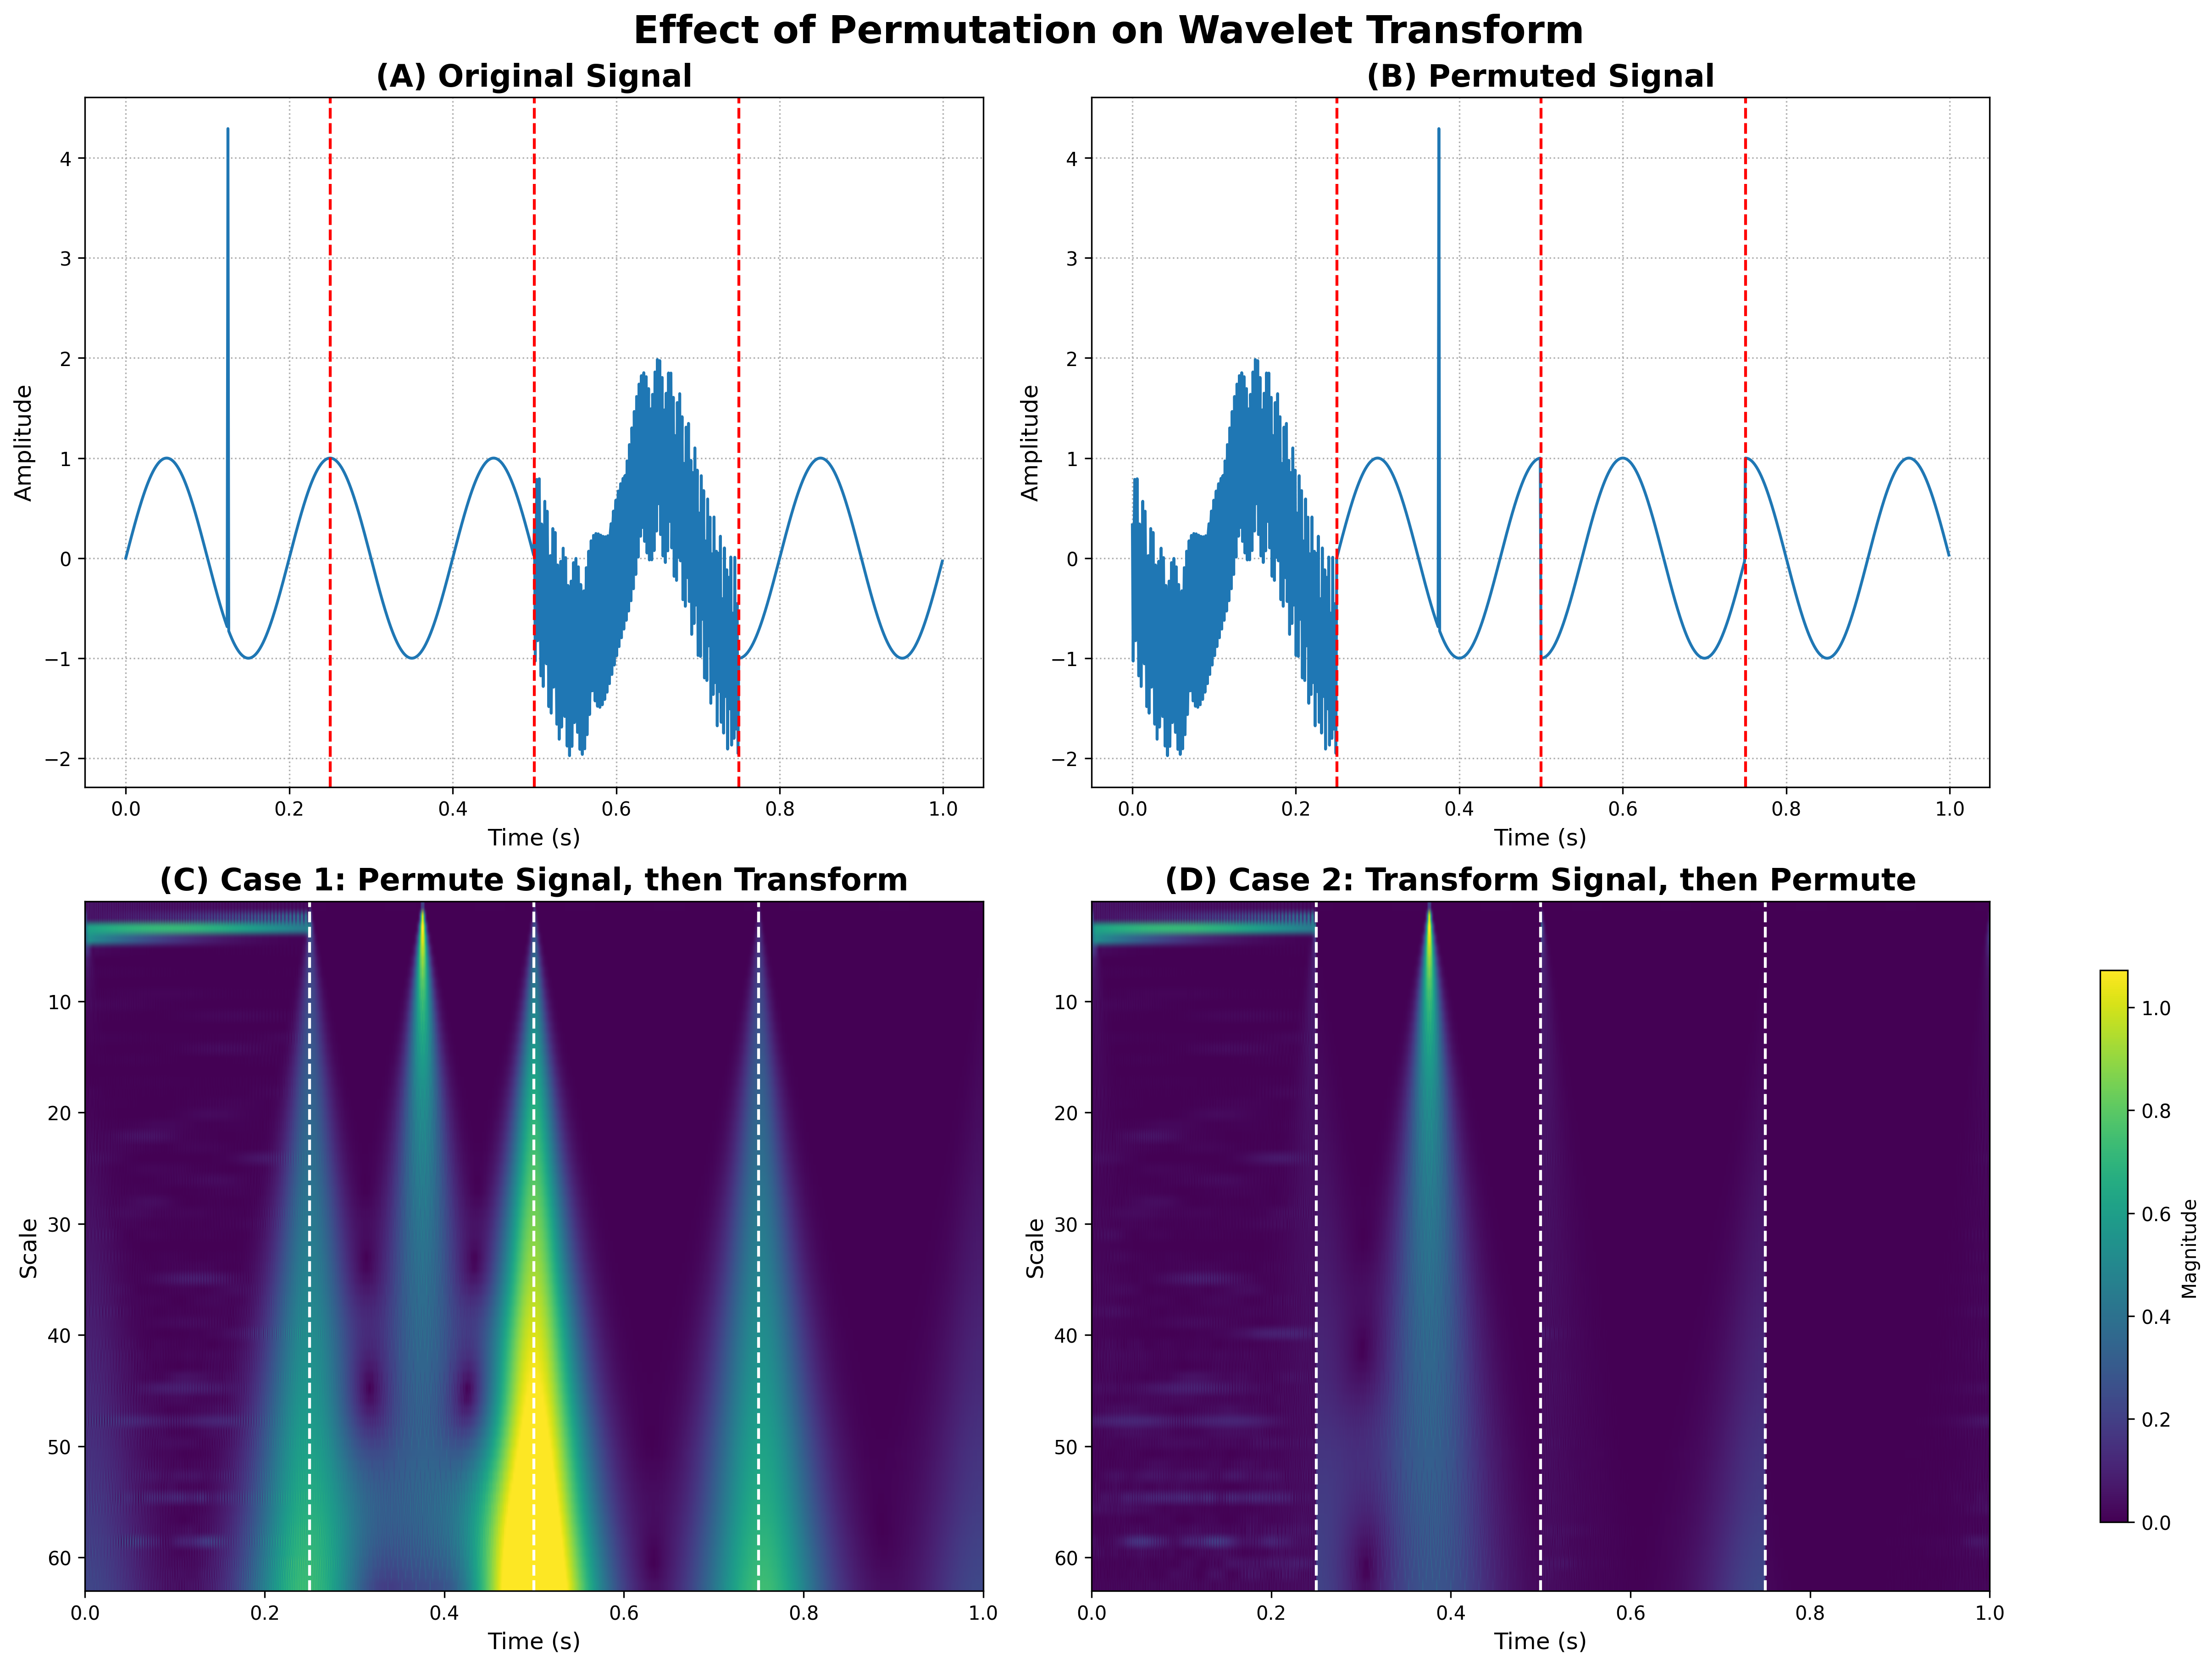
\includegraphics[width=1\textwidth]{Images/Chapter3/wavelet-permutation.png}
\caption{تاثیر ترتیب اعمال جایگشت و تبدیل موجک بر اسکالوگرام حاصل}
\label{fig:wavelet-permutation}
\end{figure}

این راهبرد یک پیش‌نیاز اساسی را به همراه دارد: تبدیلات منتخب باید به گونه‌ای باشند که ترتیب اعمال آن‌ها و تبدیل موجک، تفاوت چشمگیری در خروجی نهایی ایجاد نکند. به عبارت دیگر، نتیجه‌ی اعمال تبدیل داده‌افزایی بر روی اسکالوگرام باید تا حد امکان به نتیجه‌ی محاسبه‌ی اسکالوگرام از روی سیگنالِ داده‌افزایی‌شده نزدیک باشد. زیرا در دنیای واقعی، پدیده‌هایی مانند نویز یا چرخش حسگر، ابتدا بر سیگنال خام اثر می‌گذارند و سپس این سیگنالِ تغییریافته است که توسط ابزارهایی مانند تبدیل موجک تحلیل می‌شود.

خوشبختانه، تبدیل موجک یک تبدیل خطی است. این ویژگی ریاضی به ما اجازه می‌دهد تا تبدیلات خطی را با آن جابه‌جا کنیم بدون آنکه خروجی به شکل معناداری تغییر کند. به همین دلیل، استفاده از تبدیلات مقیاس‌دهی، معکوس‌سازی زمانی، بر زدن کانال‌ها و چرخش مشکلی ایجاد نمی‌کنند. اما نویز و جایگشت اسکالوگرام حاصل را به کلی تغییر می‌دهند. البته در رابطه با جایگشت، همانطور که در شکل \ref{fig:wavelet-permutation} قابل مشاهده است،
بخش‌های دارای فرکانس بالا (مقیاس پایین) که تغییرات محلی را در نظر می‌گیرند، تغییر چندانی ایجاد نمی‌شود اما در مقیاس‌های بالا که فرکانس‌های پایین و تغییرات سراسری را در نظر می‌گیرند، تغییرات شدیدی ایجاد می‌شود.

\section{جمع‌بندی}

در این فصل، روش پیشنهادی این پژوهش به‌طور جامع معرفی و تشریح گردید. ابتدا، معماری پایه که بر دو کدگذار مجزا برای حوزه‌های زمان و زمان-فرکانس استوار است، مورد بررسی قرار گرفت و نقاط ضعف و زمینه‌های مستعد بهبود در آن شناسایی شد. سپس، نوآوری‌های این پژوهش که برای رفع این چالش‌ها طراحی شده‌اند، ارائه گردید. نوآوری اصلی، جایگزینی چارچوب یادگیری تباینی \lr{SimCLR} با الگوریتم \lr{SwAV} بود که یک رویکرد مبتنی بر خوشه‌بندی است و با هدف یادگیری بازنمایی‌هایی پایدارتر و متمایزتر معرفی شد. علاوه بر این، راهبرد داده‌افزایی برای اسکالوگرام‌ها مورد بازنگری قرار گرفت و یک رویکرد جدید مبتنی بر تبدیلات معنادار فیزیکی که با ماهیت سیگنال‌ها سازگاری بیشتری دارد، جایگزین روش‌های پیشین شد. در فصل آتی، کارایی نوآوری‌های مطرح‌شده از طریق آزمایش‌های گسترده مورد ارزیابی قرار گرفته و نتایج حاصل از آن به تفصیل بررسی خواهد شد.

\chapter{آزمایش‌ها و نتایج}
\clearpage

در این فصل ابتدا به معرفی مجموعه داده‌های استفاده شده در انجام آزمایش‌ها می‌پردازیم. سپس به بررسی آزمایش‌های انجام شده و نتایج به‌دست‌آمده از ارزیابی مدل پیشنهادی می‌پردازیم و نتایج حاصل را مورد بررسی قرار می‌دهیم.

به‌طور کلی، آزمایش‌های انجام شده در این پژوهش را می‌توان به دو دسته تقسیم کرد:
\begin{enumerate}
    \item پیش‌آموزش خودنظارتی بر روی مجموعه داده‌ی کوچک و تنظیم دقیق بر روی همان مجموعه.
    \item پیش‌آموزش خودنظارتی بر روی مجموعه داده‌ی بزرگ و تنظیم دقیق بر روی مجموعه داده‌ی کوچک.
\end{enumerate}

\section{مجموعه داده}

برای ارزیابی عملکرد روش پیشنهادی در این پژوهش، از دو مجموعه داده \lr{HAPT\LTRfootnote{Smartphone-Based Recognition of Human Activities and Postural Transitions}}\cite{reyes2015smartphone}
(مجموعه داده کوچک) و
\lr{MobiAct}\cite{vavoulas2016mobiact}
(مجموعه داده بزرگ)
استفاده کردیم. در ادامه، جزئیات هر یک از این مجموعه داده‌ها به تفصیل تشریح می‌شود.

\subsection{مجموعه داده \lr{HAPT}}

مجموعه داده \lr{HAPT}
یکی از مجموعه داده‌های شناخته‌شده و پرکاربرد در حوزه شناسایی فعالیت انسان است که در دسترس عموم قرار دارد. این مجموعه داده نسخه توسعه‌یافته و کامل‌تری از مجموعه داده
\lr{UCI-HAR}\cite{anguita2013public}
است و علاوه بر فعالیت‌های پایه، شامل گذارهای وضعیتی\LTRfootnote{Postural Transitions} نیز می‌شود.

هدف اصلی از ایجاد این مجموعه داده، فراهم کردن داده‌های خام و پردازش‌شده از حسگرهای اینرسی تعبیه‌شده در گوشی‌های هوشمند برای ساخت و ارزیابی مدل‌های شناسایی فعالیت است. تمرکز ویژه این مجموعه داده بر تمایز قائل شدن بین فعالیت‌های ایستا و پویا و همچنین شناسایی حرکات کوتاه و انتقالی بین حالت‌های ایستا است.

\begin{figure}[htb!]
\centering
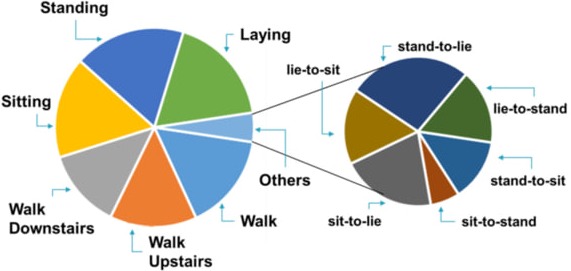
\includegraphics[width=0.75\textwidth]{Images/Chapter4/hapt-classes.png}
\caption{دسته‌های مختلف مجموعه داده \lr{HAPT}}
\label{fig:hapt-classes}
\end{figure}

داده‌های این مجموعه از ۳۰ داوطلب در بازه سنی ۱۹ تا ۴۸ سال جمع‌آوری شده است. هر شرکت‌کننده یک گوشی هوشمند \lr{Samsung Galaxy S II} را بر روی کمر خود بسته بود و رویه مشخصی از فعالیت‌ها را انجام می‌داد. تمام آزمایش‌ها به صورت ویدیویی ضبط شدند تا برچسب‌گذاری داده‌ها با دقت بالایی به صورت دستی انجام شود.

داده‌ها از دو حسگر اصلی گوشی هوشمند استخراج شده‌اند: حسگر شتاب‌سنج که سیگنال شتاب خطی سه‌محوره و حسگر ژیروسکوپ که سیگنال سرعت زاویه‌ای سه‌محوره را ثبت می‌کند. نرخ نمونه‌برداری برای هر دو حسگر ۵۰ هرتز بوده است.

همانطور که در شکل \ref{fig:hapt-classes}
می‌توان دید، این مجموعه داده شامل ۱۲ کلاس فعالیت مجزا است که به دو دسته اصلی تقسیم می‌شوند:
\begin{itemize}
    \item فعالیت‌های پایه که خود شامل سه فعالیت ایستای ایستادن، نشستن و دراز کشیدن و سه فعالیت پویای راه رفتن، بالا رفتن از پله و پایین آمدن از پله می‌باشد.
    \item گذارهای وضعیتی که شامل حرکات انتقالی بین فعالیت‌های ایستا می‌باشد و دارای فعالیت‌های ایستادن به نشستن، نشستن به ایستادن، نشستن به دراز کشیدن، دراز کشیدن به نشستن، ایستادن به دراز کشیدن و دراز کشیدن به ایستادن می‌باشد.
\end{itemize}

مجموعه داده \lr{HAPT} هم به صورت داده‌های خام حسگر و هم به صورت ویژگی‌های استخراج‌شده ارائه می‌گردد. داده‌های خام شامل سیگنال‌های سه‌محوره شتاب‌سنج و ژیروسکوپ به صورت سری زمانی است که نتیجتا شامل ۶ ویژگی می‌باشد. ویژگی‌های استخراج شده نیز بدین صورت می‌باشند که ابتدا سیگنال‌های خام با استفاده از یک پنجره لغزان به طول ۱۲۸ (۵۶.۲ ثانیه) و ۵۰ درصد همپوشانی قطعه‌بندی شده‌اند. از هر قطعه، یک بردار ویژگی ۵۶۱ بعدی استخراج شده است. این ویژگی‌ها شامل محاسبات آماری در حوزه زمان و فرکانس مانند میانگین، انحراف معیار، تبدیل فوریه سریع و غیره هستند. در این پژوهش از سیگنال‌های خام حسگرها برای آموزش مدل استفاده کردیم.

\subsection{مجموعه داده \lr{MobiAct}}

مجموعه داده \lr{MobiAct}
یک مجموعه داده عمومی برای شناسایی فعالیت انسان  است که با استفاده از حسگرهای گوشی هوشمند ایجاد شده و به طور خاص بر تشخیص فعالیت‌های روزمره و انواع سقوط\LTRfootnote{Falls}
تمرکز دارد. این مجموعه داده شامل داده‌های ثبت‌شده از سه حسگر اصلی یک گوشی هوشمند \lr{Samsung Galaxy S III}
یعنی شتاب‌سنج، ژیروسکوپ و حسگر جهت‌یاب\LTRfootnote{Orientation Sensor} می‌باشد.

داده‌ها از ۵۷ داوطلب (۴۲ مرد و ۱۵ زن) با میانگین سنی ۲۶ سال جمع‌آوری شده است. از این تعداد، ۵۰ شرکت‌کننده تمام سناریوهای مربوط به فعالیت‌های روزمره و ۵۴ شرکت‌کننده تمام سناریوهای سقوط را با موفقیت به پایان رساندند. برای شبیه‌سازی هرچه بهتر شرایط واقعی، از هر شرکت‌کننده خواسته شد تا گوشی هوشمند را به صورت آزاد و با جهت‌گیری دلخواه در جیب شلوار خود قرار دهد.

فعالیت‌های ثبت‌شده در این مجموعه داده به دو گروه اصلی تقسیم می‌شوند:
\begin{itemize}
    \item\textbf{نه نوع فعالیت روزمره:}  این فعالیت‌ها شامل ایستادن، راه رفتن، دویدن، پریدن، بالا رفتن از پله، پایین آمدن از پله، نشستن روی صندلی، وارد شدن به ماشین و خارج شدن از ماشین است.
    \item\textbf{چهار نوع سقوط شبیه‌سازی‌شده:}  این سقوط‌ها شامل سقوط به جلو، سقوط به جلو روی زانو، سقوط به پهلو و سقوط به عقب در حین تلاش برای نشستن روی صندلی می‌باشند.
\end{itemize}

\section{جزئیات پیاده‌سازی}

در این بخش به بررسی جزئیات مختلف پیاده‌سازی روش پیشنهادی (شامل پیش‌پردازش داده‌ها، آموزش مدل و معیارهای ارزیابی) می‌پردازیم.

\subsection{پیش‌پردازش داده‌ها}

پیش‌پردازش داده‌ها یک مرحله مهم در آموزش مدل‌های شناسایی فعالیت انسان است و عملکرد چشم‌گیری در بهبود نتایج به همراه دارد. برای این امر، ابتدا بایستی که داده‌ها را نرمال‌سازی کنیم. برای نرمال‌سازی داده‌ها از روش استانداردسازی که به آن نرمال‌سازی \lr{Z-score} نیز می‌گویند استفاده می‌کنیم. فرمول آن به فرم زیر است:
\begin{equation}
    z=\frac{x-\mu}{\sigma}
\end{equation}
در این رابطه $x$ بیانگر مقدار هر داده، $\mu$ بیانگر میانگین توزیع داده‌ها و $\sigma$ انحراف معیار توزیع داده‌ها می‌باشند. با استفاده از استانداردسازی، میانگین توزیع داده‌ها برابر با صفر و انحراف معیار آن‌ها برابر با یک می‌شود.

نکته‌ی مهم در رابطه با نرمال‌سازی داده‌ها این است که اگر ابتدا داده‌ی خام سیگنال‌ها را استانداردسازی کنیم و سپس تبدیل موجک را اعمال کنیم، تبدیل موجک حاصل همانطور که در شکل \ref{fig:unnormalized-wavelet}
می‌توان دید، در جاهایی که موجک استفاده شده با داده‌ی سری زمانی ورودی همبستگی بالا داشته باشد، بازه‌ی اسکالوگرام خروجی بزرگ می‌گردد و می‌تواند تا چند برابر بیشتر از داده‌ی خام سیگنال شود. به‌همین منظور، داده‌ی خام سیگنال‌ها  استانداردسازی می‌شوند و داده‌ی اسکالوگرام‌ها به‌صورت مستقل از یکدیگر استانداردسازی می‌شوند. پس از استانداردسازی داده‌ها می‌توانیم از آن‌ها برای پیش‌آموزش و آموزش مدل استفاده کنیم.

\begin{figure}[htb!]
\centering
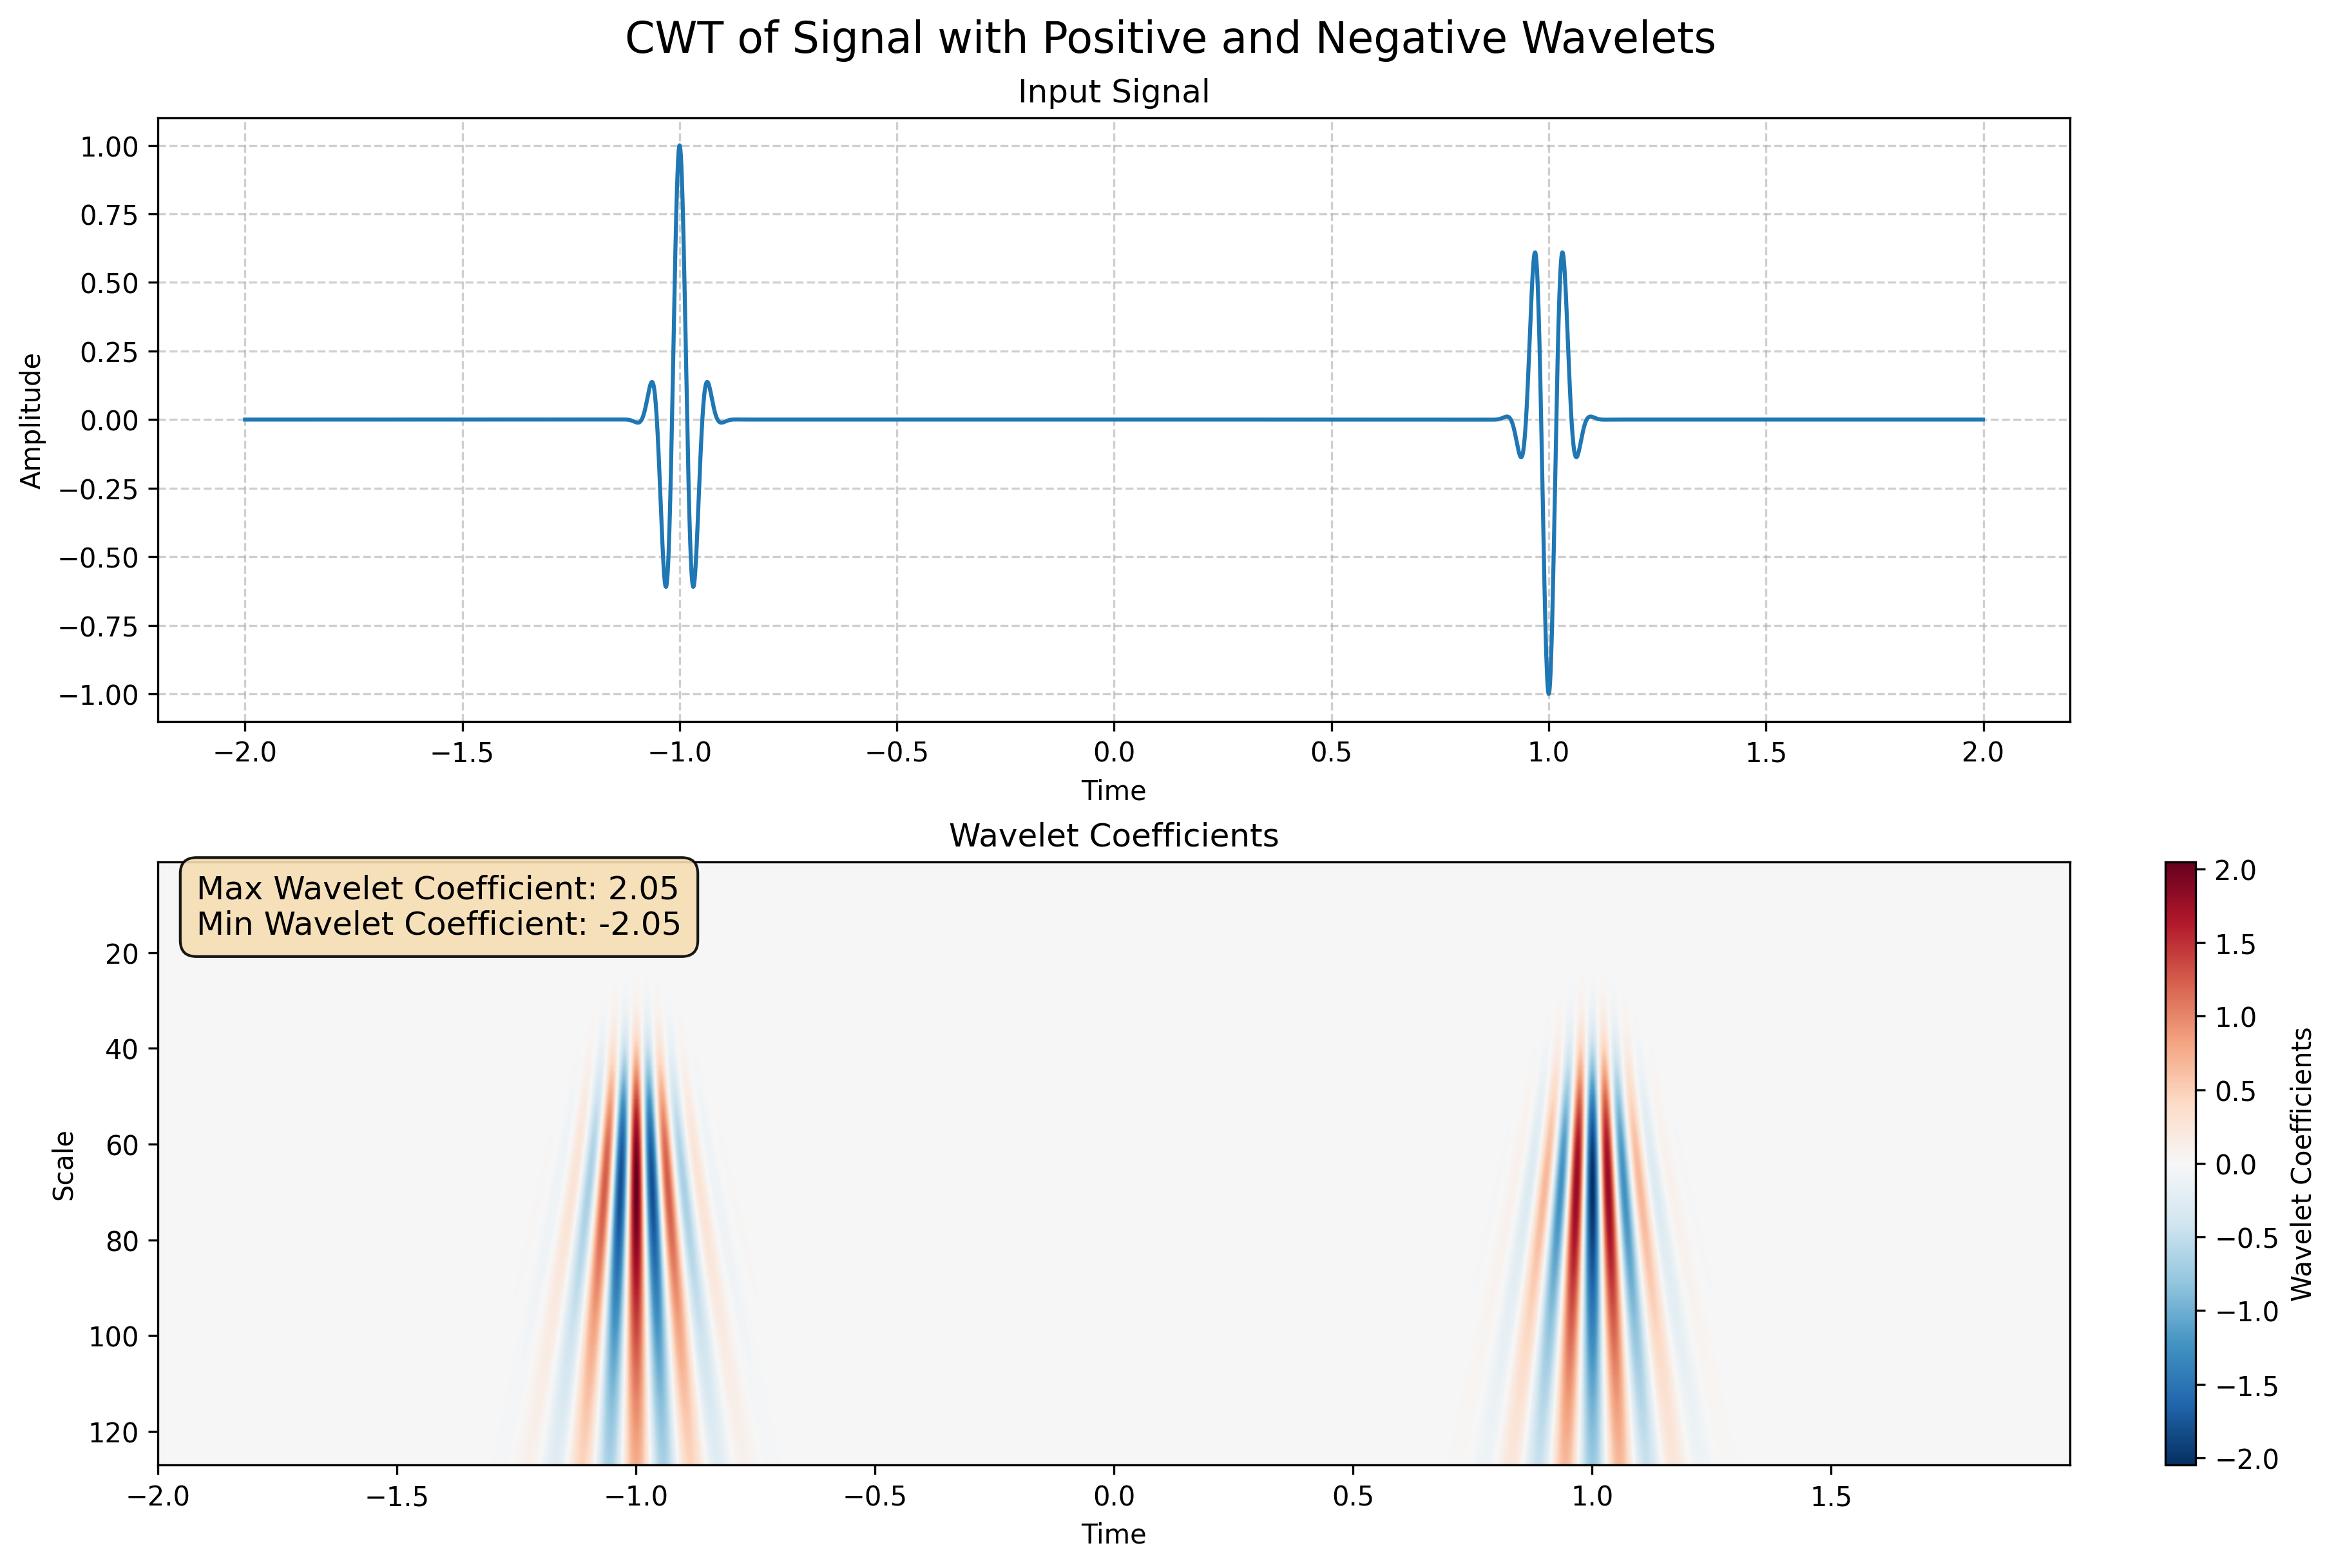
\includegraphics[width=0.75\textwidth]{Images/Chapter4/unnormalized-wavelet.png}
\caption{تاثیر تبدیل موجک بر برد اسکالوگرام خروجی}
\label{fig:unnormalized-wavelet}
\end{figure}

پس از نرمال‌سازی داده‌ها، به سراغ پر کردن مقادیر از دست رفته‌ی سیگنال‌ها با استفاده از درون‌یابی\LTRfootnote{Interpolation} می‌رویم. هر چند که هیچ یک از دو مجموعه داده‌ی استفاده شده در این پژوهش مقادیر از دست رفته ندارند، اما در هر حال می‌توان با درون‌یابی به آن‌ها رسیدگی کرد.

در قدم بعدی، بایستی نرخ نمونه‌برداری مجموعه داده‌ها را کنترل کنیم. در حالتی که هم پیش‌آموزش خودنظارتی و هم تنظیم دقیق بر روی یک مجموعه داده انجام می‌شود، نیازی به این موضوع نیست و نرخ نمونه‌برداری را همان ۵۰ هرتز
برای مجموعه داده \lr{HAPT}
نگاه می‌داریم. اما هنگامی که پیش‌آموزش بر روی مجموعه داده \lr{MobiAct}
انجام می‌شود و تنظیم دقیق بر روی \lr{HAPT}،
بایستی که هر دو مجموعه داده دارای نرخ نمونه‌برداری برابر باشند. چرا که به‌عنوان مثال اگر از یک پنجره به طول ۱۰۰ استفاده کنیم، در حالتی که نرخ نمونه‌برداری ۵۰ هرتز است، به فعالیت‌های انجام شده در یک بازه‌ی ۲ ثانیه‌ای نگاه می‌کنیم. اما هنگامی که نرخ نمونه‌برداری ۲۰ هرتز باشد (نرخ نمونه‌برداری مجموعه داده \lr{MobiAct})،
به فعالیت‌های انجام شده در یک بازه‌ی ۵ ثانیه‌ای نگاه می‌کنیم. که این امر باعث افت عملکرد مدل می‌شود. به‌همین دلیل باید در حالتی که یادگیری انتقالی انجام می‌دهیم، نرخ نمونه‌برداری مجموعه داده \lr{HAPT} را نیز به ۲۰ هرتز برسانیم تا با مجموعه داده \lr{MobiAct}
هماهنگ شود.

سپس داده‌ها را به پنجره‌های لغزان به طول ۱۲۸ و دارای همپوشانی تقسیم می‌کنیم. در رابطه با مجموعه داده \lr{HAPT} به‌علت کم بودن تعداد داده‌ها میزان همپوشانی را برابر با ۹۰ درصد قرار دادیم. اما برای مجموعه داده \lr{MobiAct} میزان همپوشانی را برابر با ۵۰ درصد قرار دادیم. در تنظیم دقیق دارای نظارت نیز برچسب هر پنجره برابر با برچسبی است که بیشترین تعداد تکرار را دارد.

\subsection{آموزش مدل}

آموزش مدل شامل دو بخش پیش‌آموزش خودنظارتی و تنظیم دقیق دارای نظارت می‌باشد. در بخش پیش‌آموزش مدل، از تمام داده‌های موجود در مجموعه داده استفاده می‌کنیم. چرا که از برچسب داده‌ها استفاده‌ای نکرده‌ایم و صرفا هدف یادگیری توزیع داده‌ها و تولید بازنمایی مفید است. بنابراین
نشت مدل\LTRfootnote{Model leakage}
رخ نمی‌دهد.

در آموزش دارای نظارت که از مجموعه داده \lr{HAPT} استفاده کرده‌ایم، مدل پیش‌آموزش دیده را با درصدهای مختلفی از داده‌ی آموزش و ارزیابی آموزش دادیم. این درصدها شامل ۸۰ درصد آموزش، ۶۰ درصد آموزش، ۴۰ درصد آموزش و ۲۰ درصد آموزش می‌باشند. در واقع هدف این است که قدرت تعمیم مدل و آموزش با میزان پایین داده‌ی آموزشی را ارزیابی کنیم.

روند انجام آزمایشات بدین صورت است که ابتدا رمزگذارهای سیگنال و اسکالوگرام را با استفاده از روشی که در فصل قبل ارائه دادیم را پیش‌آموزش می‌دهیم و وزن‌های 
رمزگذارها را ذخیره می‌کنیم. سپس در مرحله‌ی بعد، دسته‌بندها را بر روی ویژگی‌های استخراج شده از رمزگذارها با استفاده از درصدهای مختلف داده آموزشی آموزش می‌دهیم. به ازا هر درصد، ۵ بار آزمایش را به‌این صورت تکرار می‌کنیم:
\begin{enumerate}
    \item مجموعه داده را به ۵ بخش مساوی تقسیم می‌کنیم.
    \item بسته به درصد داده‌ی آموزشی و ارزیابی، تعدادی از این بخش‌ها آموزشی و تعدادی از آن‌ها ارزیابی می‌باشند.
    \item ۵ بار آزمایش را تکرار می‌کنیم و هر بار داده‌های آموزشی و ارزیابی متفاوت می‌باشند.
    \item ارزیابی نهایی عملکرد مدل برابر با میانگین ۵ بار اجرا مربوطه می‌باشد.
\end{enumerate}

\subsection{معیارهای ارزیابی}

ارزیابی عملکرد مدل‌های یکی از مهم‌ترین بخش‌های یادگیری ماشین می‌باشد. در این پژوهش از دو معیار ارزیابی امتیاز \lr{F1}\LTRfootnote{F1 Score}
و امتیاز کاپا\LTRfootnote{Kappa Score}
(که به آن کاپای کوهن\LTRfootnote{Cohen's Kappa} نیز می‌گویند) استفاده کرده‌ایم. اما پیش از بررسی این دو معیار ارزیابی، بایستی که ۳ معیار ارزیابی دیگر شامل صحت\LTRfootnote{Accuracy}، دقت\LTRfootnote{Precision} و فراخوانی\LTRfootnote{Recall} را معرفی کنیم.

معیار صحت به‌عنوان یکی از معیارهای پرکاربرد برای ارزیابی یک مدل دسته‌بندی در مسائل مختلف یادگیری ماشین مورد استفاده قرار می‌گیرد. این معیار نسبت تعداد داده‌هایی را که به درستی توسط مدل دسته‌بندی شده‌اند به تعداد کل داده‌های موجود در داده‌های آزمون می‌سنجد. فرمول محاسبه صحت به فرم معادله \ref{eq:accuracy} می‌باشد:
\begin{equation}
    \mathrm{Accuracy}=\frac{TP+TN}{TP+TN+FP+FN}
    \label{eq:accuracy}
\end{equation}
در این معادله، $TP$\LTRfootnote{True Positive} به تعداد نمونه‌های مثبت واقعی که به درستی مثبت تشخیص داده‌شده‌اند، $TN$\LTRfootnote{True Negative} به تعداد نمونه‌های منفی واقعی که به درستی منفی تشخیص داده‌شده‌اند، $FP$\LTRfootnote{False Positive} به تعداد نمونه‌های منفی واقعی که به اشتباه مثبت تشخیص داده‌شده‌اند و $FN$\LTRfootnote{False Negative} به تعداد نمونه‌های مثبت واقعی که به اشتباه به‌عنوان منفی تشخیص داده‌شده‌اند اشاره دارد.

معیار دقت بیانگر نسبت نمونه‌های مثبت واقعی که به درستی تشخیص داده‌شده‌اند به تعداد نمونه‌هایی که مدل مثبت تشخیص داده‌است می‌باشد:
\begin{equation}
    \mathrm{Precision}=\frac{TP}{TP+FP}
\end{equation}
معیار فراخوانی نیز بیانگر نسبت نمونه‌های مثبت واقعی که به درستی تشخیص داده‌شده‌اند به تعداد کل نمونه‌های مثبت واقعی است:
\begin{equation}
    \mathrm{Recall}=\frac{TP}{TP+FN}
\end{equation}
حال به بررسی معیارهای ارزیابی مورد استفاده در این پژوهش می‌پردازیم. معیار امتیاز \lr{F1}
یک معیار جامع برای ارزیابی مدل‌های دسته‌بندی است که به صورت ترکیبی از دقت و فراخوانی محاسبه می‌شود. این معیار بیشتر منعکس‌کننده‌ی توازن میان دقت و فراخوانی مدل است. فرمول محاسبه امتیاز \lr{F1} به فرم معادله \ref{eq:f1-score} می‌باشد:
\begin{equation}
    \mathrm{F1 \space Score}=2\times\frac{\mathrm{Precision}\times\mathrm{Recall}}{\mathrm{Precision}+\mathrm{Recall}}
    \label{eq:f1-score}
\end{equation}
معیار ارزیابی دیگری که در این پژوهش مورد استفاده قرار گرفته است، امتیاز کاپا می‌باشد. این معیار، میزان توافق بین پیش‌بینی‌های انجام‌شده توسط مدل و برچسب‌های واقعی را با در نظر گرفتن احتمال توافق تصادفی، ارزیابی می‌کند. مزیت اصلی امتیاز کاپا این است که نشان می‌دهد عملکرد مدل تا چه حد از یک حدس کاملاً تصادفی بهتر است. این ویژگی، کاپا را به معیاری قابل اطمینان‌تر، به‌ویژه در هنگام مواجهه با مجموعه داده‌های نامتوازن تبدیل می‌کند. فرمول محاسبه امتیاز کاپا به فرم معادله \ref{eq:kappa} می‌باشد:
\begin{equation}
\mathrm{Kappa} = \frac{\mathrm{Accuracy} - \mathrm{Accuracy_r}}{1 - \mathrm{Accuracy_r}}
\label{eq:kappa}
\end{equation}
در این معادله،
\lr{Accuracy}
همان صحت مدل است و $\mathrm{Accuracy}_r$
نشان‌دهنده‌ی صحت توافق تصادفی است. این مقدار، نمایانگر صحت عملکرد یک مدل فرضی است که تعداد پیش‌بینی‌هایش برای هر دسته، دقیقا با تعداد پیش‌بینی‌های مدل اصلی ما یکسان است، اما این تخصیص برچسب‌ها را کاملا 
به صورت تصادفی انجام می‌دهد. به عبارت دیگر، ما عملکرد مدل خود را با یک پیش‌بینی‌کننده‌ی تصادفی که از توزیع داده‌ها آگاه است، مقایسه می‌کنیم تا ببینیم یادگیری مدل چقدر فراتر از شانس بوده است. برای یک مسئله‌ی دسته‌بندی چندکلاسه با $k$
دسته، فرمول کلی محاسبه‌ی $\mathrm{Accuracy}_r$
به صورت معادله \ref{eq:acc_r_multiclass} می‌باشد:
\begin{equation}
\mathrm{Accuracy_r} = \frac{1}{N^2} \sum_{i=1}^{k} (A_i \times P_i)
\label{eq:acc_r_multiclass}
\end{equation}
در این معادله $k$ تعداد دسته‌ها، $N$ تعداد کل نمونه‌ها، $A_i$ تعداد کل نمونه‌های واقعی متعلق به دسته‌ی $i$ و $P_i$
تعداد کل نمونه‌هایی است که توسط مدل به عنوان دسته‌ی $i$ پیش‌بینی شده‌اند.

مقدار امتیاز کاپا بین ۱- و ۱+ قرار دارد. مقادیر مثبت به معنای عملکرد بهتر مدل از یک دسته‌بند تصادفی، مقدار صفر به معنای عملکرد کاملا تصادفی مدل و مقادیر منفی به معنای عملکرد بدتر مدل از یک دسته‌بند تصادفی می‌باشد.

\subsection{ابرپارامترها}

جزئیات پیکربندی مدل پیشنهادی در جدول \ref{tab:model-configs}
قابل مشاهده می‌باشد. مقادیر انتخابی بر اساس روش پایه \cite{taghanaki2023self} انتخاب شده‌اند و جستجوی گسترده‌ای برای یافتن پیکربندی بهینه انجام نشده است. تعداد خوشه‌ها برای روش \lr{SwAV} نیز به‌صورت تجربی بایستی حدود ۱۰ برابر تعداد دسته‌های مجموعه داده هدف باشند\cite{caron2020unsupervised}. بنابراین تعداد خوشه‌ها را برابر با ۱۲۸ قرار دادیم.

\begin{table}[ht]
\centering
\caption{پیکربندی یادگیرنده‌ی سیگنال (سمت راست) و یادگیرنده‌ی اسکالوگرام (سمت چپ)}
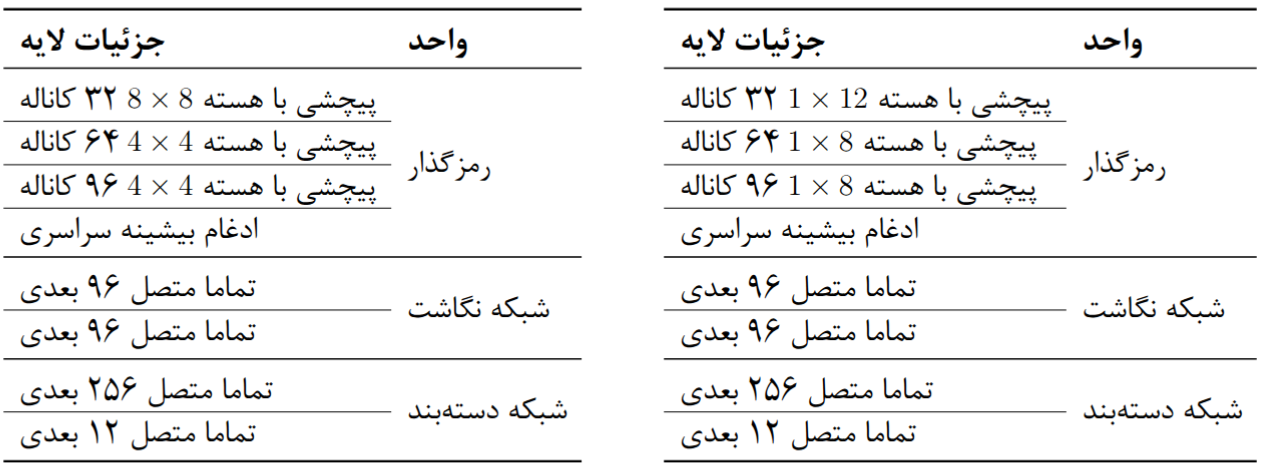
\includegraphics[width=1\textwidth]{Images/Chapter4/structure-table.png}
\label{tab:model-configs}
\end{table}

% \begin{table}[h]
% \centering
% \caption{پیکربندی یادگیرنده‌ی سیگنال (سمت راست) و یادگیرنده‌ی اسکالوگرام (سمت چپ)}
% \label{tab:model-configs}

% % ------------ جدول اول ------------
% \begin{minipage}{0.4\textwidth}
% \centering
% \renewcommand{\arraystretch}{1.2} % تنظیم فاصله عمودی بین ردیف‌ها
% \begin{tabular}{ll} % حذف خطوط عمودی
%     \toprule % خط افقی بالایی ضخیم
%     \textbf{واحد} & \textbf{جزئیات لایه} \\
%     \midrule % خط افقی میانی
%     \multirow{4}{*}{رمزگذار} & پیچشی با هسته \lr{$1 \times 12$} ۳۲ کاناله \\
%     \cline{2-2} % خط افقی فقط برای ستون دوم
%     & پیچشی با هسته \lr{$1 \times 8$} ۶۴ کاناله \\
%     \cline{2-2}
%     & پیچشی با هسته \lr{$1 \times 8$} ۹۶ کاناله \\
%     \cline{2-2}
%     & ادغام بیشینه سراسری \\
%     \midrule % خط افقی میانی
%     \multirow{2}{*}{شبکه نگاشت} & تماما متصل ۹۶ بعدی \\
%     \cline{2-2}
%     & تماما متصل ۹۶ بعدی \\
%     \midrule % خط افقی میانی
%     \multirow{2}{*}{شبکه دسته‌بند} & تماما متصل ۲۵۶ بعدی \\
%     \cline{2-2}
%     & تماما متصل ۱۲ بعدی \\
%     \bottomrule % خط افقی پایینی ضخیم
% \end{tabular}
% \end{minipage}
% \hfill % ایجاد فاصله افقی بین دو جدول
% % ------------ جدول دوم ------------
% \begin{minipage}{0.4\textwidth}
% \centering
% \renewcommand{\arraystretch}{1.2} % تنظیم فاصله عمودی بین ردیف‌ها
% \begin{tabular}{ll} % حذف خطوط عمودی
%     \toprule % خط افقی بالایی ضخیم
%     \textbf{واحد} & \textbf{جزئیات لایه} \\
%     \midrule % خط افقی میانی
%     \multirow{4}{*}{رمزگذار} & پیچشی با هسته \lr{$8 \times 8$} ۳۲ کاناله \\
%     \cline{2-2} % خط افقی فقط برای ستون دوم
%     & پیچشی با هسته \lr{$4 \times 4$} ۶۴ کاناله \\
%     \cline{2-2}
%     & پیچشی با هسته \lr{$4 \times 4$} ۹۶ کاناله \\
%     \cline{2-2}
%     & ادغام بیشینه سراسری \\
%     \midrule % خط افقی میانی
%     \multirow{2}{*}{شبکه نگاشت} & تماما متصل ۹۶ بعدی \\
%     \cline{2-2}
%     & تماما متصل ۹۶ بعدی \\
%     \midrule % خط افقی میانی
%     \multirow{2}{*}{شبکه دسته‌بند} & تماما متصل ۲۵۶ بعدی \\
%     \cline{2-2}
%     & تماما متصل ۱۲ بعدی \\
%     \bottomrule % خط افقی پایینی ضخیم
% \end{tabular}
% \end{minipage}
% \end{table}

نرخ یادگیری در بخش پیش‌آموزش خودنظارتی بدین صورت می‌باشد:
\begin{enumerate}
    \item مقدار اولیه‌ی نرخ یادگیری را برابر با $0.001$ قرار می‌دهیم.
    \item به‌صورت خطی طی ۱۰ دوره\LTRfootnote{Epoch} اول آن را تا $0.05$ افزایش می‌دهیم. مقادیر بزرگ‌تر موجب ناپایداری یادگیری می‌شوند.
    \item به صورت کسینوسی و تا آخرین دوره آموزش (۱۰۰ دوره) مقدار نرخ یادگیری را تا $0.0001$ کاهش می‌دهیم.
\end{enumerate}
برای تنظیم دقیق مدل، از یک نرخ یادگیری ثابت برابر با $0.001$ استفاده کردیم.
تعداد تکرار الگوریتم سینکهورن (که در بخش \ref{sec:sinkhorn} معرفی کردیم) برابر با ۳ می‌باشد.

مقدار ابرپارمتر $\epsilon$ (معادله \ref{eq:swav-optimal-transport}) را برابر با 0.01 قرار دادیم. افزایش مقدار این پارامتر باعث می‌شود که تخصیص‌های روش سینکهورن برای تمامی داده‌ها به تمامی خوشه‌ها یکنواخت شود که در این حالت مدل بازنمایی‌های خوبی یاد نمی‌گیرد. پارامتر دما ($\tau$ در معادله \ref{eq:swav-p-calculation}) نیز می‌تواند تاثیری مشابه داشته باشد. زیاد کردن مقدار آن باعث می‌شود که توزیع تخصیص‌ها توسط مدل (نه الگوریتم سینکهورن) یکنواخت شود. اما بیش از حد کم کردن مقدار آن نیز شدیدا باعث ناپایداری آموزش خواهد شد. همانطور که در معادله \ref{eq:swav-p-calculation} دیده می‌شود،
مقدار موجود در نمای $exp$ تقسیم بر ابرپارمتر دما می‌شود. کوچک بودن بیش از حد این ابرپارامتر باعث می‌شود که مقدار این توان از لحاظ عددی بسیار بزرگ شود که به تبع آن کامپیوتر نمی‌تواند مقدار آن را محاسبه کند و فرآیند آموزش دچار  خطا می‌شود. بنابراین مقدار آن را برابر با مقدار 0.05 قرار دادیم که هم از یکنواخت شدن توزیع سینکهورن جلوگیری می‌کند و هم باعث ناپایداری آموزش نمی‌شود.

اندازه‌ی دسته برای داده‌های خام سیگنال را برابر با ۱۰۲۴ و برای اسکالوگرام نیز برابر با ۵۱۲ قرار دادیم. تعداد دوره‌ی آموزش در بخش پیش‌آموزش خودنظارتی را برای رمزگذار سیگنال برابر با ۱۰۰ و برای رمزگذار اسکالوگرام برابر با ۷۵ قرار دادیم. اما برای تنظیم دقیق هر دو مدل، از روش توقف زودهنگام\LTRfootnote{Early Stopping}
استفاده می‌کنیم. بدین صورت که بر روی داده‌های اعتبارسنجی، مقدار هزینه مدل را بررسی می‌کنیم و هنگامی که مدل دچار بیش‌برازش شد و هزینه‌ی اعتبارسنجی بالا رفت، آموزش را متوقف می‌کنیم و بهترین مدل را انتخاب می‌کنیم.

\section{نتایج}

در این بخش، به ارائه و تحلیل نتایج حاصل از آزمایش‌های انجام‌شده بر روی مدل پیشنهادی پرداخته می‌شود. همانطور که پیش‌تر تشریح شد، ارزیابی عملکرد مدل در دو سناریوی اصلی صورت گرفته است. ابتدا، نتایج حاصل از پیش‌آموزش خودنظارتی و تنظیم دقیق بر روی مجموعه داده واحد \lr{HAPT}
در قالب آزمایش‌های درون‌مجموعه‌ای\LTRfootnote{Intra-Dataset} بررسی می‌گردد.
سپس، کارایی روش در سناریوی یادگیری انتقالی، که در آن پیش‌آموزش بر روی مجموعه داده \lr{MobiAct}
و تنظیم دقیق بر روی مجموعه داده \lr{HAPT}
انجام شده، تحت عنوان آزمایش‌های بین‌مجموعه‌ای\LTRfootnote{Inter-Dataset} ارائه می‌گردد.
عملکرد مدل در تمامی آزمایش‌ها با استفاده از معیارهای امتیاز
\lr{F1}
و امتیاز کاپا سنجیده شده و نتایج به تفکیک مورد بحث قرار خواهند گرفت.

\subsection{نتایج آزمایش‌های درون‌مجموعه‌ای}

در این بخش، به بررسی نتایج حاصل از سناریوی اول، یعنی پیش‌آموزش خودنظارتی و تنظیم دقیق مدل بر روی مجموعه داده‌ی \lr{HAPT}
می‌پردازیم. هدف از این آزمایش، ارزیابی عملکرد مدل در مقایسه با مدل پایه و یادگیری دارای نظارت و ایجاد یک خط معیار برای مقایسه با نتایج یادگیری انتقالی است که در بخش بعد ارائه خواهد شد.

نتایج دقیق این آزمایش‌ها در جدول
\ref{tab:intra-dataset-comparison}
ارائه شده است. این جدول، میانگین و انحراف معیار امتیاز
\lr{F1}
و امتیاز کاپا را به ازای استفاده از ۲۰، ۴۰، ۶۰ و ۸۰ درصد از داده‌های آموزشی برچسب‌دار، پس از ۵ بار تکرار آزمایش، نمایش می‌دهد

% \begin{LTR}
% \begin{table}[ht]
% \centering
% \caption{نتایج عملکرد مدل در سناریوی درون‌مجموعه‌ای بر اساس درصدهای مختلف داده آموزشی}
% \label{tab:intra-dataset-comparison}
% \begin{tabular}{llll}
%     \toprule
%     \textbf{\lr{Labeled Data (\%)}} & \textbf{\lr{Method}} & \textbf{\lr{F1-Score}} & \textbf{\lr{Kappa Score}} \\
%     \midrule
%     \multirow{3}{*}{\lr{20\%}} 
%     & \lr{Fully Supervised} & \lr{$0.XX \pm 0.XX$} & \lr{$0.XX \pm 0.XX$} \\
%     & \lr{Baseline \cite{taghanaki2023self}} & \lr{$0.XX \pm 0.XX$} & \lr{\textbf{$0.XX \pm 0.XX$}} \\
%     & \lr{Proposed Method (Ours)} & \lr{\textbf{$0.XX \pm 0.XX$}} & \lr{$0.XX \pm 0.XX$} \\
%     \midrule
%     \multirow{3}{*}{\lr{40\%}} 
%     & \lr{Fully Supervised} & \lr{$0.XX \pm 0.XX$} & \lr{$0.XX \pm 0.XX$} \\
%     & \lr{Baseline \cite{taghanaki2023self}} & \lr{$0.XX \pm 0.XX$} & \lr{$0.XX \pm 0.XX$} \\
%     & \lr{Proposed Method (Ours)} & \lr{\textbf{$0.XX \pm 0.XX$}} & \lr{\textbf{$0.XX \pm 0.XX$}} \\
%     \midrule
%     \multirow{3}{*}{\lr{60\%}} 
%     & \lr{Fully Supervised} & \lr{$0.XX \pm 0.XX$} & \lr{$0.XX \pm 0.XX$} \\
%     & \lr{Baseline \cite{taghanaki2023self}} & \lr{$0.XX \pm 0.XX$} & \lr{$0.XX \pm 0.XX$} \\
%     & \lr{Proposed Method (Ours)} & \lr{\textbf{$0.XX \pm 0.XX$}} & \lr{\textbf{$0.XX \pm 0.XX$}} \\
%     \midrule
%     \multirow{3}{*}{\lr{80\%}} 
%     & \lr{Fully Supervised} & \lr{$0.XX \pm 0.XX$} & \lr{$0.XX \pm 0.XX$} \\
%     & \lr{Baseline \cite{taghanaki2023self}} & \lr{$0.XX \pm 0.XX$} & \lr{$0.XX \pm 0.XX$} \\
%     & \lr{Proposed Method (Ours)} & \lr{\textbf{$0.XX \pm 0.XX$}} & \lr{\textbf{$0.XX \pm 0.XX$}} \\
%     \bottomrule
% \end{tabular}
% \end{table}
% \end{LTR}

\begin{table}[ht]
\centering
\caption{نتایج عملکرد مدل در سناریوی درون‌مجموعه‌ای بر اساس درصدهای مختلف داده آموزشی}
\label{tab:intra-dataset-comparison}
\begin{tabular}{clll}
    \toprule
    \textbf{درصد داده} & \textbf{روش} & \textbf{امتیاز \lr{F1}} & \textbf{امتیاز کاپا} \\
    \midrule
    \multirow{3}{*}{\%۲۰} 
    & کاملا نظارت‌شده & $0.439 \pm 0.006$ & $0.316 \pm 0.007$ \\
    & روش پایه \cite{taghanaki2023self} & $0.645 \pm 0.005$ & $0.554 \pm 0.008$ \\
    & روش پیشنهادی & $\boldsymbol{0.658 \pm 0.005}$ & $\boldsymbol{0.571 \pm 0.007}$ \\
    \midrule
    \multirow{3}{*}{\%۴۰} 
    & کاملا نظارت‌شده & $0.619 \pm 0.008$ & $0.521 \pm 0.008$ \\
    & روش پایه \cite{taghanaki2023self} & $\boldsymbol{0.807 \pm 0.008}$ & $\boldsymbol{0.758 \pm 0.011}$ \\
    & روش پیشنهادی & $0.806 \pm 0.009$ & $0.757 \pm 0.011$ \\
    \midrule
    \multirow{3}{*}{\%۶۰} 
    & کاملا نظارت‌شده & $0.770 \pm 0.008$ & $0.710 \pm 0.010$ \\
    & روش پایه \cite{taghanaki2023self} & $0.876 \pm 0.006$ & $0.847 \pm 0.007$ \\
    & روش پیشنهادی & $\boldsymbol{0.895 \pm 0.003}$ & $\boldsymbol{0.872 \pm 0.004}$ \\
    \midrule
    \multirow{3}{*}{\%۸۰} 
    & کاملا نظارت‌شده & $0.893 \pm 0.007$ & $0.869 \pm 0.008$ \\
    & روش پایه \cite{taghanaki2023self} & $0.914 \pm 0.013$ & $0.896 \pm 0.016$ \\
    & روش پیشنهادی & $\boldsymbol{0.923 \pm 0.007}$ & $\boldsymbol{0.907 \pm 0.009}$ \\
    \bottomrule
\end{tabular}
\end{table}

\begin{figure}[ht!]
    \centering
    \begin{subfigure}[b]{0.49\textwidth}
        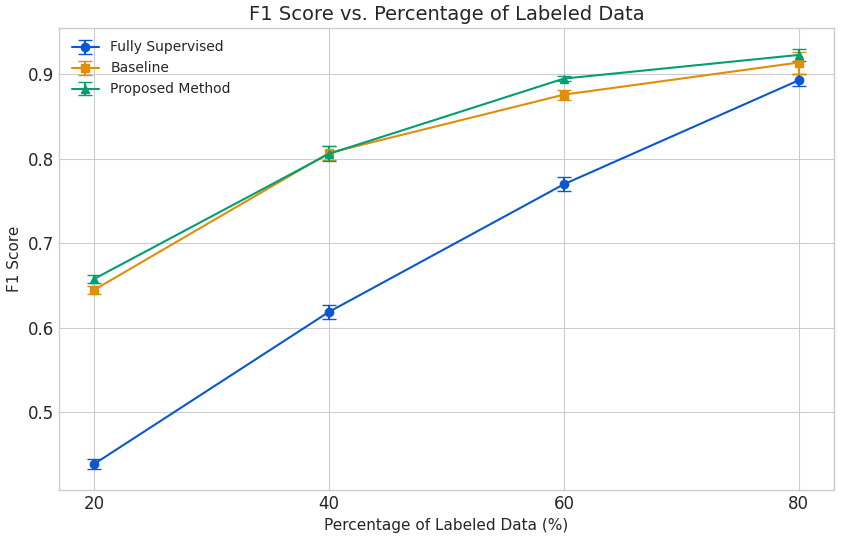
\includegraphics[width=\textwidth]{Images/Chapter4/main-results-f1.png}
    \end{subfigure}
    \hfill % ایجاد فاصله بین دو عکس
    \begin{subfigure}[b]{0.49\textwidth}
        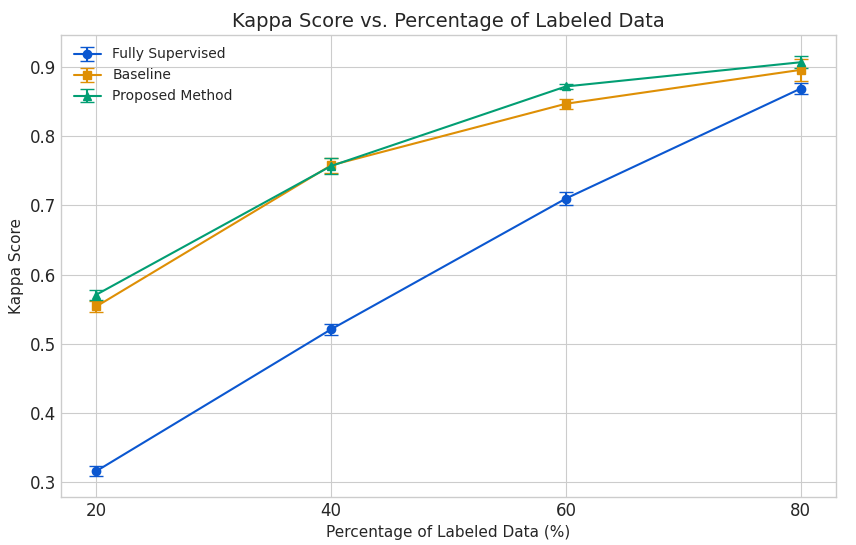
\includegraphics[width=\textwidth]{Images/Chapter4/main-results-kappa.png}
    \end{subfigure}
    \caption{مقایسه امتیاز \lr{F1} (راست) و امتیاز کاپا (چپ) برای روش‌های مختلف بر اساس درصدهای متفاوت داده‌های آموزشی.}
    \label{fig:main-results}
\end{figure}

اولین و واضح‌ترین نتیجه‌گیری که از روی جدول \ref{tab:intra-dataset-comparison} و شکل \ref{fig:main-results} می‌توان استنباط کرد، عملکرد به مراتب بهتر هر دو روش خودنظارتی (روش پایه و روش پیشنهادی) در مقایسه با روش کاملا نظارت‌شده است؛ به‌ویژه در شرایط کمبود داده‌های برچسب‌دار. برای مثال، در حالت استفاده از تنها \%۲۰ داده‌ها، روش پیشنهادی بهبودی در حدود \%۲۲ در امتیاز \lr{F1} نسبت به مدل کاملاً نظارت‌شده نشان می‌دهد.
این شکاف عمیق، ارزش مرحله پیش‌آموزش را به اثبات می‌رساند؛ جایی که مدل با استفاده از کل داده‌های برچسب‌نخورده، بازنمایی‌های غنی و مفیدی را می‌آموزد و با یک دانش اولیه قدرتمند وارد مرحله تنظیم دقیق می‌شود.

با تمرکز بر مقایسه دو روش خودنظارتی، مشاهده می‌شود که روش پیشنهادی در اکثر سناریوها (\%۲۰، \%۶۰ و \%۸۰ داده) عملکرد بهتری از خود نشان داده است.
\begin{itemize}
    \item \textbf{در شرایط داده بسیار کم (\%۲۰)}: روش پیشنهادی با اختلاف کمی، بهترین عملکرد را ثبت کرده است. این موضوع اهمیت ویژه‌ای دارد، زیرا نشان می‌دهد مدل پیشنهادی در چالش‌برانگیزترین حالت (کمبود داده) کارآمدتر است. این موضوع نشان می‌دهد که مدل پیشنهادی قابلیت تعمیم‌پذیری بیشتری می‌تواند از خود نشان بدهد.
    \item \textbf{در شرایط داده متوسط (\%۴۰):} عملکرد دو روش بسیار نزدیک و رقابتی است و روش پایه برتری جزئی و از نظر آماری نامحسوسی دارد. این نشان می‌دهد که هر دو روش در این سطح از داده به پایداری عملکردی خوبی رسیده‌اند.
    \item \textbf{در شرایط داده زیاد (\%۶۰ و \%۸۰):} با افزایش حجم داده‌های برچسب‌دار، برتری روش پیشنهادی مجدداً خود را نشان می‌دهد و به ویژه در سطح ۶۰٪، شکاف قابل توجهی ایجاد می‌کند. این امر نشان‌دهنده ظرفیت بالاتر مدل پیشنهادی برای بهره‌برداری از داده‌های بیشتر و رسیدن به دقت بالاتر است.
\end{itemize}
در مجموع، نتایج این بخش به وضوح نشان می‌دهد که روش پیشنهادی نه تنها بر محدودیت‌های یادگیری کاملا نظارت‌شده در شرایط کمبود داده فائق می‌آید، بلکه در مقایسه مستقیم با روش پایه‌ی اخیر نیز در اکثر موارد عملکردی بهتر ارائه می‌دهد. این نتایج، پتانسیل بالای مدل را در سناریوی درون-مجموعه‌ای تأیید می‌کند. در بخش بعد، این ارزیابی را یک گام فراتر برده و عملکرد مدل را در سناریوی چالش‌برانگیزتر یادگیری انتقالی خواهیم سنجید.

\subsection{نتایج آزمایش‌های بین‌مجموعه‌ای}

در این بخش، به بررسی نتایج حاصل از سناریوی دوم، یعنی پیش‌آموزش خودنظارتی بر روی مجموعه داده \lr{MobiAct} و تنظیم دقیق مدل بر روی مجموعه داده‌ی \lr{HAPT}
می‌پردازیم. نتایج دقیق این آزمایش‌ها در جدول
\ref{tab:inter-dataset-comparison}
ارائه شده است. این جدول، میانگین و انحراف معیار امتیاز
\lr{F1}
و امتیاز کاپا را به ازای استفاده از ۲۰، ۴۰، ۶۰ و ۸۰ درصد از داده‌های آموزشی برچسب‌دار، پس از ۵ بار تکرار آزمایش، نمایش می‌دهد

\begin{table}[ht]
\centering
\caption{نتایج عملکرد مدل در سناریوی بین‌مجموعه‌ای بر اساس درصدهای مختلف داده آموزشی}
\label{tab:inter-dataset-comparison}
\begin{tabular}{clll}
    \toprule
    \textbf{درصد داده} & \textbf{روش} & \textbf{امتیاز \lr{F1}} & \textbf{امتیاز کاپا} \\
    \midrule
    \multirow{3}{*}{\%۲۰} 
    & کاملا نظارت‌شده & $0.439 \pm 0.006$ & $0.316 \pm 0.007$ \\
    & روش پایه \cite{taghanaki2023self} & $0.591 \pm 0.006$ & $0.489 \pm 0.007$ \\
    & روش پیشنهادی & $\boldsymbol{0.602 \pm 0.006}$ & $\boldsymbol{0.560 \pm 0.008}$ \\
    \midrule
    \multirow{3}{*}{\%۴۰} 
    & کاملا نظارت‌شده & $0.619 \pm 0.008$ & $0.521 \pm 0.008$ \\
    & روش پایه \cite{taghanaki2023self} & $0.743 \pm 0.010$ & $0.676 \pm 0.011$ \\
    & روش پیشنهادی & $\boldsymbol{0.763 \pm 0.011}$ & $\boldsymbol{0.701 \pm 0.015}$ \\
    \midrule
    \multirow{3}{*}{\%۶۰} 
    & کاملا نظارت‌شده & $0.770 \pm 0.008$ & $0.710 \pm 0.010$ \\
    & روش پایه \cite{taghanaki2023self} & $0.831 \pm 0.007$ & $0.789 \pm 0.009$ \\
    & روش پیشنهادی & $\boldsymbol{0.863 \pm 0.007}$ & $\boldsymbol{0.830 \pm 0.009}$ \\
    \midrule
    \multirow{3}{*}{\%۸۰} 
    & کاملا نظارت‌شده & $0.893 \pm 0.007$ & $0.869 \pm 0.008$ \\
    & روش پایه \cite{taghanaki2023self} & $0.887 \pm 0.007$ & $0.863 \pm 0.008$ \\
    & روش پیشنهادی & $\boldsymbol{0.902 \pm 0.004}$ & $\boldsymbol{0.886 \pm 0.006}$ \\
    \bottomrule
\end{tabular}
\end{table}

\begin{figure}[ht!]
    \centering
    \begin{subfigure}[b]{0.49\textwidth}
        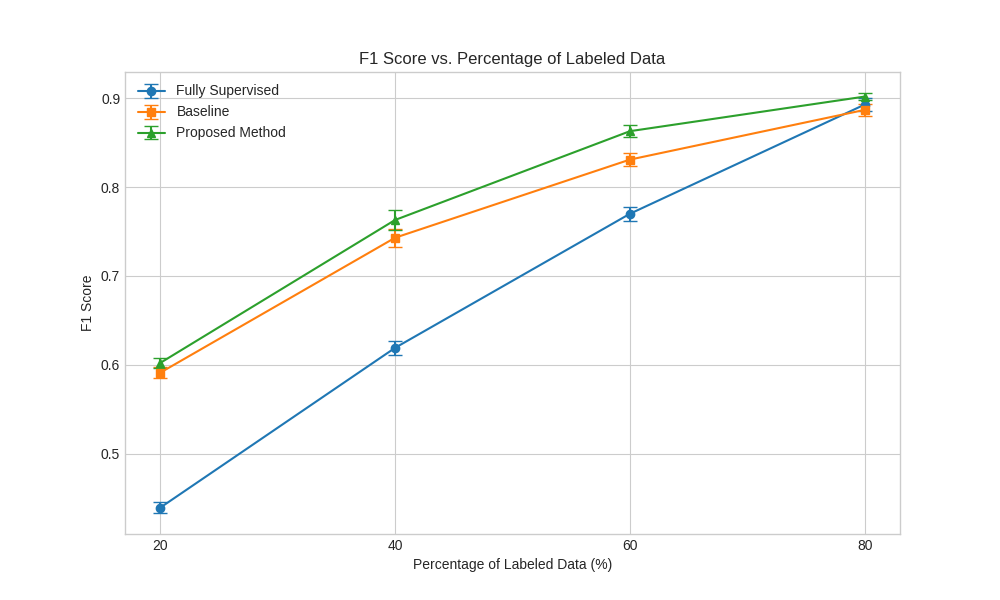
\includegraphics[width=\textwidth]{Images/Chapter4/transfer-results-f1.png}
    \end{subfigure}
    \hfill % ایجاد فاصله بین دو عکس
    \begin{subfigure}[b]{0.49\textwidth}
        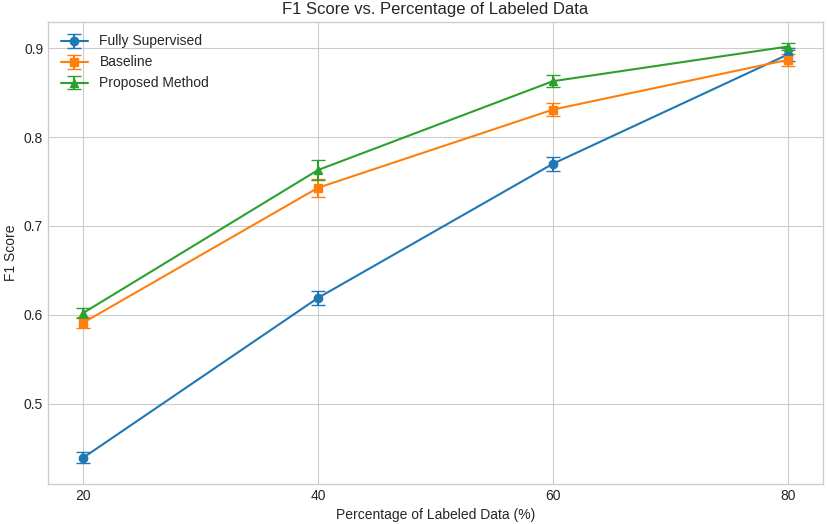
\includegraphics[width=\textwidth]{Images/Chapter4/transfer-results-kappa.png}
    \end{subfigure}
    \caption{مقایسه امتیاز \lr{F1} (راست) و امتیاز کاپا (چپ) برای روش‌های مختلف بر اساس درصدهای متفاوت داده‌های آموزشی.}
    \label{fig:transfer-results}
\end{figure}

تحلیل نتایج ارائه شده در جدول \ref{tab:inter-dataset-comparison}، به ویژه هنگامی که در کنار نتایج آزمایش‌های درون-مجموعه‌ای (جدول \ref{tab:intra-dataset-comparison}) قرار می‌گیرد، یافته‌های بسیار مهمی را در مورد قدرت تعمیم و پایداری مدل‌ها آشکار می‌سازد.

اولین مشاهده در تحلیل این جدول، برتری کامل و مداوم روش پیشنهادی بر هر دو روش دیگر در تمامی سطوح داده‌ی برچسب‌دار است. برخلاف سناریوی قبلی که در سطح \%۴۰ داده، رقابت بسیار نزدیک بود، در این سناریوی بین-مجموعه‌ای، مدل پیشنهادی در تمام آزمون‌ها با اختلاف معناداری بهترین عملکرد را به ثبت رسانده است. این موضوع نشان می‌دهد که بازنمایی‌های آموخته‌شده توسط روش پیشنهادی از مجموعه داده \lr{MobiAct}، برای انتقال به دامنه جدید (مجموعه داده \lr{HAPT}) کارآمدتر و قابل‌استفاده‌تر بوده‌اند.

نکته کلیدی و بسیار قابل تأمل، مقایسه مستقیم عملکرد مدل‌ها بین دو سناریو است. مشاهده می‌شود که امتیازات \lr{F1} و کاپا برای هر دو روش خودنظارتی در سناریوی بین‌مجموعه‌ای به طور کلی کمتر از سناریوی درون‌مجموعه‌ای است. مجموعه داده‌های \lr{MobiAct} و \lr{HAPT} اگرچه هر دو به شناسایی فعالیت انسان می‌پردازند، اما در جزئیاتی نظیر
نوع و محل قرارگیری سنسورها، مجموعه فعالیت‌های ثبت‌شده و مشخصات شرکت‌کنندگان تفاوت‌هایی دارند. این تفاوت‌ها باعث ایجاد اختلاف در توزیع آماری داده‌ها شده و باعث می‌شود بازنمایی‌های آموخته‌شده از یک دامنه، به طور کامل به دامنه‌ی دیگر قابل انتقال نباشند.

با این حال، با وجود اینکه هر دو روش خودنظارتی تحت تاثیر تغییر دامنه دچار افت عملکرد شدند، اما میزان این افت برای روش پایه به مراتب شدیدتر بوده است. این یافته نشان می‌دهد که روش پیشنهادی مقاومت بیشتری در برابر تغییر دامنه دارد و قادر به یادگیری بازنمایی‌های عمومی‌تر و مستقل از دامنه است. در حالی که روش پایه ممکن است ویژگی‌هایی را آموخته باشد که بیش از حد به خصوصیات مجموعه داده \lr{MobiAct} وابسته بوده‌اند، روش پیشنهادی توانسته است الگوهای کلی‌تری را استخراج کند که حتی پس از انتقال به یک دامنه جدید نیز کارایی بالاتری از خود نشان می‌دهند.

در نهایت، نتایج این بخش نشان می‌دهد که اگرچه فرضیه ساده "پیش‌آموزش روی داده بیشتر همیشه بهتر است" به دلیل وجود شکاف دامنه به چالش کشیده می‌شود، اما همین چالش، نقطه قوت اصلی روش پیشنهادی را آشکار می‌سازد: پایداری\LTRfootnote{Robustness} و قابلیت تعمیم بالاتر در شرایط واقعی که داده‌های آموزش و آزمون ممکن است از توزیع‌های متفاوتی آمده باشند. این ویژگی، ارزش عملیاتی مدل پیشنهادی را به شدت افزایش می‌دهد.

\section{جزئیات اجرا}

برای آموزش مدل‌ها از یک کارت گرافیک \lr{NVIDIA Tesla P100} استفاده شده است. جزئیات زمان اجرای پیش‌آموزش مدل‌ها به شرح زیر می‌باشد:
\begin{itemize}
    \item \textbf{مجموعه داده \lr{HAPT}:} هر دوره از پیش‌آموزش رمزگذار سیگنال حدود ۱۲۵ ثانیه و هر دوره از پیش‌آموزش رمزگذار اسکالوگرام حدود ۲۶۰ ثانیه به‌طول انجامید. نتیجتا پیش‌آموزش کامل رمزگذار سیگنال حدود ۳ و نیم ساعت و رمزگذار اسکالوگرام حدود ۵ و نیم ساعت به‌طول انجامید.
    \item \textbf{مجموعه داده \lr{MobiAct}:} هر دوره از پیش‌آموزش رمزگذار سیگنال حدود ۱۳۰۰ ثانیه و هر دوره از پیش‌آموزش رمزگذار اسکالوگرام حدود ۲۸۰۰ ثانیه به‌طول انجامید. نتیجتا پیش‌آموزش کامل رمزگذار سیگنال حدود ۳۶ ساعت و رمزگذار اسکالوگرام حدود ۵۸ ساعت به‌طول انجامید.
\end{itemize}

یکی از معیارهای کلیدی برای نظارت بر فرآیند پیش‌آموزش و اطمینان از یادگیری بازنمایی‌های مفید، رصد کردن مقدار تابع هزینه روش \lr{SwAV} بود. اگر مقدار این تابع هزینه به عدد ثابت
$\log(K)$ (که در آن $K$ تعداد خوشه‌ها است) نزدیک شود، این امر نشان‌دهنده‌ی عدم یادگیری بازنمایی‌های معنادار توسط مدل است. دلیل این پدیده به شرح زیر است:

تابع هزینه \lr{SwAV}، همانطور که در معادله \ref{eq:swav-cross-entropy} نشان داده شد، بر اساس آنتروپی متقاطع عمل می‌کند. در این میان، بردار احتمال $p$ از خروجی یک تابع سافت‌مکس بر روی امتیازات شباهت بین بازنمایی شبکه ($z$) و مراکز خوشه‌ها به دست می‌آید (معادله \ref{eq:swav-p-calculation}). در صورتی که مدل در حال یادگیری نباشد (مثلاً به دلیل تنظیم نامناسب ابرپارامترها)، بازنمایی خروجی آن حاوی اطلاعات مفیدی نخواهد بود. در نتیجه، امتیاز شباهت این بازنمایی با تمام $K$
مرکز خوشه تقریبا یکسان خواهد بود. هنگامی که ورودی‌های یک تابع سافت‌مکس مقادیر یکسانی داشته باشند، خروجی آن یک توزیع احتمال یکنواخت خواهد بود، یعنی $p_k \approx \frac{1}{K}$ برای تمام خوشه‌ها. با جایگزین کردن $p_k$ در فرمول هزینه داریم:
\begin{equation}
    L = - \sum_{k=1}^{K} q_k \log \left( \frac{1}{K} \right) = \log(K) \sum_{k=1}^{K} q_k
\end{equation}
و از آنجا که $q$ نیز خود یک توزیع احتمال است، جمع تمام $q_k$ برابر با ۱ می‌شود و مقدار نهایی هزینه به فرم $L = \log(K)$ در می‌آید. بنابراین، وقتی مدل یادگیری را به درستی انجام نمی‌دهد، هزینه به پایین‌ترین حد ممکن برای یک حدس تصادفی، یعنی 
$\log(K)$ می‌رسد.

بنابراین، مقدار $\log(K)$ به عنوان خط پایه برای یک مدل تصادفی\LTRfootnote{Random Baseline} عمل می‌کند. در یک آموزش موفق، انتظار می‌رود که مقدار هزینه به سرعت از این عدد فاصله گرفته و به سمت مقادیر کمتر کاهش یابد. نزدیک شدن یا باقی ماندن هزینه در این سطح، هشداری مبنی بر عدم یادگیری مدل است.

\section{جمع‌بندی}

در این فصل، عملکرد مدل پیشنهادی از طریق مجموعه‌ای از آزمایش‌های جامع مورد ارزیابی قرار گرفت. ابتدا، مجموعه داده‌های مورد استفاده به عنوان بستر آزمایش‌ها معرفی شدند و سپس جزئیات پیاده‌سازی، شامل مراحل پیش‌پردازش داده‌ها، فرآیند آموزش دومرحله‌ای، ابرپارامترها و معیارهای ارزیابی تشریح گردید. نتایج در دو سناریوی اصلی ارائه شد: درون‌مجموعه‌ای و بین‌مجموعه‌ای. در سناریوی درون‌مجموعه‌ای، برتری آشکار رویکرد خودنظارتی پیشنهادی نسبت به یادگیری کاملا نظارت‌شده، به‌ویژه در شرایط کمبود داده، به اثبات رسید و در اکثر موارد عملکرد بهتری نسبت به روش پایه داشت. مهم‌تر از آن، در سناریوی چالش‌برانگیز بین‌مجموعه‌ای (یادگیری انتقالی)، مدل پیشنهادی پایداری و قابلیت تعمیم بالاتری از خود به نمایش گذاشت و با اختلاف معناداری نسبت به روش پایه، برتری خود را در تمام سطوح داده‌های برچسب‌دار تثبیت کرد. این یافته‌ها نشان می‌دهد که مدل پیشنهادی قادر به یادگیری بازنمایی‌های غنی، عمومی و مقاوم در برابر تغییر دامنه است.

\chapter{جمع‌بندي و نتيجه‌گيري و پیشنهادات}
\clearpage
در این فصل، ابتدا به جمع‌بندی و مرور کلی پژوهش انجام‌شده، اهداف، رویکردها و دستاوردهای کلیدی آن می‌پردازیم. سپس، با تکیه بر نتایج به‌دست‌آمده و محدودیت‌های موجود، پیشنهاداتی برای پژوهش‌های آتی در این حوزه ارائه خواهیم داد.

\section{جمع‌بندی}

مسئله‌ی شناسایی فعالیت انسان با استفاده از داده‌های حسگر، یکی از ارکان اساسی در توسعه‌ی سیستم‌های هوشمند مراقبتی، خانه‌های هوشمند و سلامت دیجیتال به شمار می‌رود. با وجود موفقیت‌های چشمگیر روش‌های یادگیری عمیق در این حوزه، وابستگی شدید آن‌ها به حجم زیادی از داده‌های برچسب‌دار، یک چالش اساسی و پرهزینه محسوب می‌شود. فرآیند برچسب‌گذاری داده‌های حسگری نه تنها زمان‌بر و نیازمند نیروی متخصص است، بلکه مدل‌های آموزش‌دیده به روش نظارت‌شده اغلب در تعمیم به افراد جدید یا شرایط متغیر دنیای واقعی، با افت عملکرد مواجه می‌شوند.

این پژوهش با هدف غلبه بر این محدودیت‌ها، به بررسی و پیاده‌سازی یک چارچوب یادگیری خودنظارتی برای استخراج بازنمایی‌های غنی و تعمیم‌پذیر از سیگنال‌های مربوط به فعالیت انسان پرداخت. معماری پایه، که بر دو رمزگذار مجزا برای تحلیل همزمان داده‌ها در حوزه‌ی زمان (سیگنال خام) و حوزه‌ی زمان-فرکانس (اسکالوگرام) استوار بود، به عنوان نقطه شروع انتخاب شد. با این حال، با تحلیل این معماری، دو حوزه اصلی برای بهبود شناسایی و مورد هدف قرار گرفت.

نوآوری نخست، جایگزینی الگوریتم یادگیری تباینی \lr{SimCLR} با روش پیشرفته‌تر و مبتنی بر خوشه‌بندی \lr{SwAV} بود. این الگوریتم با بهره‌گیری از یک سازوکار پیش‌بینی تعویض‌شده و خوشه‌بندی برخط، مدل را به یادگیری بازنمایی‌هایی پایدارتر و متمایزتر وادار می‌کند که نسبت به تغییرات و تبدیلات داده‌افزایی، نامتغیر هستند. نوآوری دوم، بازنگری و بهبود راهبرد داده‌افزایی برای اسکالوگرام‌ها بود. به جای استفاده از تبدیلات اقتباس‌شده از حوزه‌ی بینایی کامپیوتر که فاقد معنای فیزیکی روشنی برای داده‌های حسگری هستند، مجموعه‌ای از تبدیلات معنادارتر و سازگارتر با ماهیت سیگنال‌ها به کار گرفته شد.

برای ارزیابی عملکرد روش پیشنهادی، دو سناریوی آزمایشی جامع طراحی گردید. در سناریوی درون‌مجموعه‌ای، که پیش‌آموزش و تنظیم دقیق بر روی مجموعه داده‌ی واحد \lr{HAPT} انجام شد، نتایج نشان داد که رویکرد خودنظارتی پیشنهادی، به ویژه در شرایط کمبود داده‌های برچسب‌دار، برتری چشمگیری نسبت به یادگیری کاملاً نظارت‌شده دارد و در اکثر موارد، عملکردی بهتر از روش پایه ارائه می‌دهد. مهم‌تر از آن، در سناریوی چالش‌برانگیزتر بین‌مجموعه‌ای که به منظور سنجش قدرت یادگیری انتقالی طراحی شده بود (پیش‌آموزش بر روی مجموعه داده‌ی بزرگ \lr{MobiAct} و تنظیم دقیق بر روی \lr{HAPT})، برتری مدل پیشنهادی کاملا مشهود بود. در این سناریو که شبیه‌ساز شرایط واقعی‌تر با وجود تغییر دامنه بین داده‌های آموزشی و ارزیابی است، مدل پیشنهادی پایداری و قابلیت تعمیم بالاتری از خود به نمایش گذاشت. این یافته‌ی کلیدی نشان می‌دهد که بازنمایی‌های آموخته‌شده توسط روش پیشنهادی، عمومی‌تر، بنیادی‌تر و در برابر تغییر دامنه مقاوم‌تر هستند.این یافته‌ی کلیدی نشان می‌دهد که بازنمایی‌های آموخته‌شده توسط روش پیشنهادی، عمومی‌تر، بنیادی‌تر و در برابر تغییر دامنه مقاوم‌تر هستند.

در مجموع، نتایج این پژوهش تأیید می‌کند که ترکیب الگوریتم یادگیری خودنظارتی \lr{SwAV} با راهبردهای داده‌افزایی متناسب، منجر به توسعه‌ی مدلی قدرتمندتر و قابل‌اطمینان‌تر برای شناسایی فعالیت انسان می‌شود که گامی مؤثر در جهت کاهش وابستگی به داده‌های برچسب‌دار و افزایش کارایی مدل‌ها در کاربردهای دنیای واقعی است.

\section{کارهای آتی}

با توجه به نتایج امیدوارکننده‌ی این پژوهش، مسیرهای متعددی برای توسعه و بهبود کارهای آتی قابل تصور است که در ادامه به برخی از مهم‌ترین آن‌ها اشاره می‌شود:
\begin{itemize}
    \item \textbf{به‌کارگیری معماری‌های پیشرفته‌تر:} رمزگذار‌های استفاده‌شده در این پژوهش مبتنی بر شبکه‌های پیچشی نسبتا ساده بودند. می‌توان با بهره‌گیری از معماری‌های پیشرفته‌تر مانند مدل مبدل که توانایی بالایی در مدل‌سازی وابستگی‌های طولانی‌مدت دارند، یا معماری‌های ترکیبی مانند \lr{CNN-LSTM}، بازنمایی‌های دقیق‌تری از الگوهای زمانی پیچیده استخراج کرد.
    \item \textbf{راهبردهای ادغام چندوجهی:} در این پژوهش از راهبرد ادغام دیرهنگام برای ترکیب خروجی دو رمزگذار استفاده شد. تحقیق بر روی راهبردهای ادغام زودهنگام یا میانی، که در آن‌ها بازنمایی‌های حوزه‌ی زمان و زمان-فرکانس در لایه‌های پایین‌تر با یکدیگر ترکیب می‌شوند، می‌تواند به مدل اجازه دهد تا وابستگی‌های متقابل میان این دو حوزه را بهتر بیاموزد.
    \item \textbf{شخصی‌سازی و یادگیری مداوم:} مدل فعلی به صورت عمومی آموزش دیده است. یک مسیر تحقیقاتی ارزشمند، توسعه‌ی روش‌هایی برای شخصی‌سازی سریع مدل برای یک کاربر جدید با استفاده از حجم بسیار کمی داده یا تطبیق مداوم مدل با تغییرات تدریجی در الگوهای حرکتی یک فرد در طول زمان (یادگیری برخط) است.
    \item \textbf{ارزیابی در سناریوهای پیچیده‌تر:} عملکرد مدل را می‌توان در مجموعه داده‌های پیچیده‌تر و نزدیک‌تر به واقعیت ارزیابی کرد؛ مجموعه داده‌هایی که شامل فعالیت‌های همزمان و هم‌پوشان، تعداد بیشتری از دسته‌های فعالیت، یا داده‌های حاصل از منابع متنوع‌تری (مانند حسگرهای محیطی در کنار حسگرهای پوشیدنی) هستند.
\end{itemize}

% \chapter{موارد به‌روزرسانی}
\section{ استفاده از \lr{subfigure}}
برای شکل‌های 
\ref{fig:fig1} و \ref{fig:fig2}
به کد مراجعه نمایید
\begin{figure}[h!]
		\centering % <-- added
		\begin{subfigure}{0.33\textwidth}
			\includegraphics[width=\linewidth]{Images/Chapter6/test1.jpg}
			\caption{\lr{test1}}
			\label{f61}
		\end{subfigure}\hfil % <-- 
		\begin{subfigure}{0.33\textwidth}
			\includegraphics[width=\linewidth]{Images/Chapter6/test2.jpg}
			\caption{\lr{test2}}
			\label{f62}
		\end{subfigure}\hfil % <-- added
        \begin{subfigure}{0.33\textwidth}
			\includegraphics[width=\linewidth]{Images/Chapter6/test3.jpg}
			\caption{\lr{test3}}
			\label{f63}
        \end{subfigure}
		\caption{دانشگاه امیرکبیر}
		\label{fig:fig1}
\end{figure}
 \begin{figure}[ht]
		\centering % <-- added
		\begin{subfigure}{0.45\textwidth}
			\includegraphics[width=\linewidth, height=0.2\textheight]{Images/Chapter6/test5.jpg}
			\caption{\lr{test5}}
			\label{f64}
		\end{subfigure}\hfil % <-- added
		\begin{subfigure}{0.45\textwidth}
			\includegraphics[width=\linewidth, height=0.2\textheight]{Images/Chapter6/test6.jpg}
			\caption{\lr{test6}}
			\label{f65}
		\end{subfigure}
		\caption{پلی تکنبیک}
		\label{fig:fig2}
\end{figure}
\section{فرض}
\begin{asum}
     برای استفاده از فرض کافیست از فرمت زیر استفاده کنید
\begin{latin}
     \normalsize
     \begin{verbatim}
    \begin{asum}
    
    \end{asum}
    \end{verbatim}
\end{latin}
\section{جدول }
\subsection{چندسطری}
مثالی از جدول چند سطری را می‌توانید در \ref{Table1} مشاهده نمایید.
\begin{table}[ht]
    \centering
    \caption{مقایسه الگوریتم‌های بهینه‌ساز}
    \begin{tabular}{|c|c|c|c|} \hline 
        \label{Table1}
        & سناریو & تعداد پارامترها  & تابع هزینه\\  
        \hline
        \multirow{4}{*}{\lr{GWO}} & 1 & 11 & $2.4241$     \\
        & 2 & 8 & $9.1389$           \\
        & 3 & 7 & $6.3343$     \\
        & 4 & 4 & $1.61788$     \\\hline
        \multirow{4}{*}{\lr{PSO}} & 1 & 11 & $20.5801$ \\
        & 2 & 8 & $10.1402$\\
        & 3 & 7 & $3.83659$ \\
        & 4 & 4 & $4.86521$\\\hline
        \multirow{4}{*}{\lr{GA}}  & 1 & 11 & $34.8627$\\
        & 2 & 8 & $33.7109$\\
        & 3 & 7 & $26.4257$\\
        & 4 & 4 & $25.6392$\\\hline						
    \end{tabular}
\end{table}
\end{asum}
\subsection{مقیاس بندی}
برای تنظیم جدول می‌توانید از دستور زیر استفاده نمایید
\begin{latin}
     \normalsize
     \begin{verbatim}
    \adjustbox{max width=\textwidth,max totalheight=\textheight, keepaspectratio}{
    \begin{tabular}...
    .
    .
    .
    \end{tabular}}
    \end{verbatim}
\end{latin}
یا 
\begin{latin}
     \normalsize
     \begin{verbatim}
    \adjustbox{width=\columnwidth,max totalheight=\textheight, keepaspectratio}{
    \begin{tabular}...
    .
    .
    .
    \end{tabular}}
    \end{verbatim}
\end{latin}
نمونه جدول بدون تنظیم
\begin{table}[ht]
    \begin{tabular}{|c|c|c|c|c|c|c|c|c|c|c|c|c|} \hline 
        & $c_1^{\alpha}$ & $c_2^{\alpha}$ & $c_1^{\gamma}$ & $c_2^{\gamma}$ & $d$ & $k$ & $d_{L_2}$ & $d_{L_3}$ & $d_{L_4}$ & $d_{\varepsilon}$ & \lr{SW} & $N$\\  
        \hline
        مثلث  & $6.6$ & $2.4$ & $4.3$ & $11.2$ & $8.6603$ & $1.07$ & $15.3696$ & $24.9362$ & $35.9237$ & $1.5$ & 110 & 58  \\\hline
        پنج شلعی  & $6.1$ & $2.8$ & $4.9$ & $12.7$ & $5.8779$ & $1.09$ & $13.2074$ & $20.6509$ & $29.0499$ & $0.9$ & 75 & 72 \\\hline
        شش ضلعی  & $5.9$ & $2.3$ & $5.2$ & $13.3$ & $5$ & $1.1$& $11.2349$ & $17.5667$ & $23.9169$ & 1 & 70 & 72 \\\hline
    \end{tabular}
    \centering
    \caption{پارامترهای الگوریتم}
    \label{Table2}
\end{table}\\
نمونه جدول با تنظیم سایز
\begin{table}[ht]
\adjustbox{max width=\textwidth,max totalheight=\textheight, keepaspectratio}{%
    \begin{tabular}{|c|c|c|c|c|c|c|c|c|c|c|c|c|} \hline 
        & $c_1^{\alpha}$ & $c_2^{\alpha}$ & $c_1^{\gamma}$ & $c_2^{\gamma}$ & $d$ & $k$ & $d_{L_2}$ & $d_{L_3}$ & $d_{L_4}$ & $d_{\varepsilon}$ & \lr{SW} & $N$\\  
        \hline
        مثلث  & $6.6$ & $2.4$ & $4.3$ & $11.2$ & $8.6603$ & $1.07$ & $15.3696$ & $24.9362$ & $35.9237$ & $1.5$ & 110 & 58  \\\hline
        پنج شلعی  & $6.1$ & $2.8$ & $4.9$ & $12.7$ & $5.8779$ & $1.09$ & $13.2074$ & $20.6509$ & $29.0499$ & $0.9$ & 75 & 72 \\\hline
        شش ضلعی  & $5.9$ & $2.3$ & $5.2$ & $13.3$ & $5$ & $1.1$& $11.2349$ & $17.5667$ & $23.9169$ & 1 & 70 & 72 \\\hline
    \end{tabular}}
    \centering
    \caption{پارامترهای الگوریتم}
    \label{Table3}
\end{table}
\begin{table}[ht]
\adjustbox{width=\columnwidth,max totalheight=\textheight, keepaspectratio}{%
    \begin{tabular}{|c|c|c|c|c|c|c|c|c|c|c|c|c|} \hline 
        & $c_1^{\alpha}$ & $c_2^{\alpha}$ & $c_1^{\gamma}$ & $c_2^{\gamma}$ & $d$ & $k$ & $d_{L_2}$ & $d_{L_3}$ & $d_{L_4}$ & $d_{\varepsilon}$ & \lr{SW} & $N$\\  
        \hline
        مثلث  & $6.6$ & $2.4$ & $4.3$ & $11.2$ & $8.6603$ & $1.07$ & $15.3696$ & $24.9362$ & $35.9237$ & $1.5$ & 110 & 58  \\\hline
        پنج شلعی  & $6.1$ & $2.8$ & $4.9$ & $12.7$ & $5.8779$ & $1.09$ & $13.2074$ & $20.6509$ & $29.0499$ & $0.9$ & 75 & 72 \\\hline
        شش ضلعی  & $5.9$ & $2.3$ & $5.2$ & $13.3$ & $5$ & $1.1$& $11.2349$ & $17.5667$ & $23.9169$ & 1 & 70 & 72 \\\hline
    \end{tabular}}
    \centering
    \caption{پارامترهای الگوریتم}
    \label{Table4}
\end{table}
\subsection{استفاده از قضیه}
\begin{theorem}
تست
\end{theorem}
\begin{proof}
    تست
\end{proof}
برای تغییر کلمه برهان به اثبات، می‌توانید خط 52 در  \lr{commands.tex} را غیر فعال نمایید.
\\
  اشکال هر سطح از  \lr{itemize} را می توانید با مراجعه به
 \lr{commands.tex} تغییر دهید، کامنت‌های مربوطه برای اینکار مشخص شده است (خطوط 44 تا 50).\\
نمونه‌ای از \lr{itemize} چهار سطحی:
\begin{itemize}
    \item تست
    \begin{itemize}
        \item تست
        \begin{itemize}
            \item تست
            \begin{itemize}
                \item تست
            \end{itemize}
        \end{itemize}
    \end{itemize}
\end{itemize}



%--------------------------------------------------------------------------appendix( مراجع و پیوست ها)
\chapterfont{\vspace*{-2em}\centering\LARGE}%

\appendix
\bibliographystyle{unsrt-fa}
\bibliography{references}
% \chapter*{‌پیوست}
\markboth{پیوست}{}
\addcontentsline{toc}{chapter}{پیوست}
موضوعات مرتبط با متن گزارش پایان نامه كه در يكی از گروه‌های زير قرار می‌گيرد، در بخش پيوست‌ها آورده شوند:
\begin{enumerate}
\item  اثبات های رياضی يا عمليات رياضی طولانی‌.‌
\item داده و اطلاعات نمونه (های) مورد مطالعه (\lr{Case Study}) چنانچه طولانی باشد‌.‌
\item نتايج كارهای ديگران چنانچه نياز به تفصيل باشد‌.‌
\item مجموعه تعاريف متغيرها و پارامترها، چنانچه طولانی بوده و در متن به انجام نرسيده باشد‌.‌
\end{enumerate}
% براي شماره‌گذاري روابط، جداول و اشكال موجود در پيوست‌ از ساختار متفاوتي نسبت به متن اصلي استفاده مي‌شود كه در زير به‌عنوان نمونه نمايش داده شده‌است. 
% \begin{equation}
%F=ma
%\end{equation}
\section*{کد میپل }
\begin{latin}
\begin{verbatim}

with(DifferentialGeometry):
with(Tensor):
DGsetup([x, y, z], M)
																	frame name: M
a := evalDG(D_x)
																	D_x
b := evalDG(-2 y z D_x+2 x D_y/z^3-D_z/z^2)


\end{verbatim}
\end{latin}
%--------------------------------------------------------------------------dictionary(واژه نامه ها)
%اگر مایل به داشتن صفحه واژه‌نامه نیستید، خط زیر را غیر فعال کنید.
% \parindent=0pt
% %
\chapter*{واژه‌نامه‌ی فارسی به انگلیسی}
\pagestyle{style9}

\addcontentsline{toc}{chapter}{واژه‌نامه‌ی فارسی به انگلیسی}
%%%%%%
\begin{multicols*}{2}

{\bf آ}
\vspace*{3mm}


\farsiTOenglish{اسکالر}{Scalar}


\vspace*{3mm}
{\bf ب}
\vspace*{3mm}

\farsiTOenglish{بالابر}{Lift}


\vspace*{3mm}
{\bf پ}
%%\vspace*{3mm}

\farsiTOenglish{پایا}{Invariant}



\vspace*{3mm}
{\bf ت}
%%\vspace*{3mm}

\farsiTOenglish{ تناظر }{Correspondence}


\vspace*{3mm}
{\bf ث}
%%\vspace*{3mm}

\farsiTOenglish{ثابت‌ساز}{Stabilizer}

\vspace*{3mm}
{\bf ج}
%%\vspace*{3mm}

\farsiTOenglish{جایگشت}{Permutation}



\vspace*{3mm}
{\bf چ}
%%\vspace*{3mm}


\farsiTOenglish{چند جمله‌ای }{Polynomial}

\vspace*{3mm}
{\bf ح}
%%\vspace*{3mm}

\farsiTOenglish{حاصل‌ضرب دکارتی}{Cartesian product}


\vspace*{3mm}
{\bf خ}
%%\vspace*{3mm}

\farsiTOenglish{خودریختی}{Automorphism}

\vspace*{3mm}
{\bf د}
%%\vspace*{3mm}

\farsiTOenglish{درجه}{Degree}


\vspace*{3mm}
{\bf ر}
%%\vspace*{3mm}


\farsiTOenglish{ریزپردازنده}{microprocessor}


\vspace*{3mm}
{\bf ز}
%%\vspace*{3mm}


\farsiTOenglish{زیرمدول}{Submodule}


\vspace*{3mm}
{\bf س}
%%\vspace*{3mm}

\farsiTOenglish{سرشت}{Character}


\vspace*{3mm}
{\bf ص}
%%\vspace*{3mm}

\farsiTOenglish{صادقانه}{Faithful}

\vspace*{3mm}
{\bf ض}
%%\vspace*{3mm}

\farsiTOenglish{ضرب داخلی}{Inner product}

\vspace*{3mm}
{\bf ط}
%%\vspace*{3mm}


\farsiTOenglish{طوقه}{Loop}


\vspace*{3mm}
{\bf ظ}
%%\vspace*{3mm}


\farsiTOenglish{ظرفیت}{Valency}
 
\vspace*{3mm}
{\bf ع}
%%\vspace*{3mm}


\farsiTOenglish{عدم مجاورت}{Nonadjacency}



\vspace*{3mm}
{\bf ف}
%%\vspace*{3mm}

\farsiTOenglish{فضای برداری}{Vector space}



\vspace*{3mm}
{\bf ک}
%%\vspace*{3mm}

\farsiTOenglish{کاملاً تحویل‌پذیر}{Complete reducibility}


\vspace*{3mm}
{\bf گ}
%%\vspace*{3mm}


\farsiTOenglish{گراف}{Graph}



\vspace*{3mm}
{\bf م}
%%\vspace*{3mm}

\farsiTOenglish{ماتریس جایگشتی}{Permutation matrix }


\vspace*{3mm}
{\bf ن}
%%\vspace*{3mm}

\farsiTOenglish{ناهمبند}{Disconnected}


\vspace*{3mm}
{\bf و}
%%\vspace*{3mm}

\farsiTOenglish{وارون‌پذیر}{Invertible}


\vspace*{3mm}
{\bf ه}
%%\vspace*{3mm}

\farsiTOenglish{همبند}{Connected}



\vspace*{3mm}
{\bf ی}
%%\vspace*{3mm}

\farsiTOenglish{یال}{Edge}




\end{multicols*}%
% %%%%%%
\chapter*{ واژه‌نامه‌ی انگلیسی به فارسی}
\pagestyle{style9}
\lhead{\thepage}\rhead{واژه‌نامه‌ی انگلیسی به فارسی}
\addcontentsline{toc}{chapter}{واژه‌نامه‌ی انگلیسی به فارسی}

\LTRmulticolcolumns
\begin{multicols}{2}
{\hfill\bf  \lr{A}}
%%\vspace*{1.5mm}

\englishTOfarsi{Automorphism}{خودریختی}

\vspace*{3mm}
{\hfill\bf   \lr{B}}
%%\vspace*{1.5mm}

\englishTOfarsi{Bijection}{دوسویی}

\vspace*{3mm}
{\hfill\bf   \lr{C}}
%%\vspace*{1.5mm}

\englishTOfarsi{Cycle group}{گروه دوری}

\vspace*{3mm}
{\hfill\bf   \lr{D}}
%%\vspace*{1.5mm}

\englishTOfarsi{Degree}{درجه}

\vspace*{3mm}
{\hfill\bf   \lr{E}}
%%\vspace*{1.5mm}

\englishTOfarsi{Edge}{یال}

\vspace*{3mm}
{\hfill\bf   \lr{F}}
%%\vspace*{1.5mm}

\englishTOfarsi{Function}{تابع}

\vspace*{3mm}
{\hfill\bf   \lr{G}}
%%\vspace*{1.5mm}

\englishTOfarsi{Group}{گروه}

\vspace*{3mm}
{\hfill\bf   \lr{H}}
%%\vspace*{1.5mm}

\englishTOfarsi{Homomorphism}{همریختی}

\vspace*{3mm}
{\hfill\bf   \lr{I}}
%%\vspace*{1.5mm}

\englishTOfarsi{Invariant}{پایا}

\vspace*{3mm}
{\hfill\bf   \lr{L}}
%%\vspace*{1.5mm}

\englishTOfarsi{Lift}{بالابر}

\vspace*{3mm}
{\hfill\bf   \lr{M}}
%%\vspace*{1.5mm}

\englishTOfarsi{Module}{مدول}

\vspace*{3mm}
{\hfill\bf   \lr{N}}
%%\vspace*{1.5mm}

\englishTOfarsi{Natural map}{نگاشت طبیعی}

\vspace*{3mm}
{\hfill\bf   \lr{O}}
%%\vspace*{1.5mm}

\englishTOfarsi{One to One}{یک به یک}

\vspace*{3mm}
{\hfill\bf   \lr{P}}
%%\vspace*{1.5mm}

\englishTOfarsi{Permutation group}{گروه جایگشتی}

\vspace*{3mm}
{\hfill\bf   \lr{Q}}
%%\vspace*{1.5mm}

\englishTOfarsi{Quotient graph}{گراف خارج‌قسمتی}

 \vspace*{3mm}
{\hfill\bf   \lr{R}}
%%\vspace*{1.5mm}

\englishTOfarsi{Reducible}{تحویل پذیر}

\vspace*{3mm}
{\hfill\bf   \lr{S}}
%%\vspace*{1.5mm}

\englishTOfarsi{Sequence}{دنباله}

 \vspace*{3mm}
{\hfill\bf   \lr{T}}
%%\vspace*{1.5mm}

\englishTOfarsi{Trivial character}{سرشت بدیهی}

\vspace*{3mm}
{\hfill\bf   \lr{U}}
%%\vspace*{1.5mm}

\englishTOfarsi{Unique}{منحصربفرد}

\vspace*{3mm}
{\hfill\bf   \lr{V}}
%%\vspace*{1.5mm}

\englishTOfarsi{Vector space}{فضای برداری}
\end{multicols}
%--------------------------------------------------------------------------index(نمایه)
%اگر مایل به داشتن صفحه نمایه نیستید، خط زیر را غیر فعال کنید.
\pagestyle{style7}
\printindex
\pagestyle{style7}
%کلمات کلیدی انگلیسی
\latinkeywords{Human Activity Recognition, Self-Supervised Learning, Wavelet Transform, Contrastive Learning, Transfer Learning}
%چکیده انگلیسی

\en-abstract{With the increasing expansion of smart environments and the use of various sensors such as mobile phones, the need for systems that can automatically and accurately recognize human activities has grown. One of the main challenges in this field is the heavy reliance of machine learning models on labeled data, the collection of which on a large scale is costly and time-consuming. This issue highlights the necessity of utilizing methods that can extract conceptual and transferable representations from sensor data without the need for manual labeling. In this research, a self-supervised learning framework has been designed that, by leveraging a combination of temporal and frequency perspectives, attempts to extract high-quality and general representations from raw human activity data. The proposed framework, aiming to improve data representation quality, reduce the need for labeled data, and enhance model generalizability, has been evaluated in two different scenarios: first, training and evaluation in the same environment; and second, training in one environment and evaluating in a different one, with the goal of assessing the model's knowledge transfer and generalization capabilities. The evaluation results show that the proposed framework has achieved \textbf{92.3\% F1 score} (with a \textbf{0.9\% improvement} over the base model) in the direct training scenario on the HAPT dataset, and \textbf{90.2\% F1 score} (with a \textbf{1.5\% improvement} over the base model) in the transfer learning scenario from the MobiAct dataset to the HAPT dataset. By utilizing the combination of temporal and frequency information, this framework has been able to extract representations that have led to improved accuracy in human activity recognition. Overall, the proposed method takes an effective step towards reducing dependency on labeled data and developing generalizable models for application in diverse and real-world environments.}
%%%%%%%%%%%%%%%%%%%%% کدهای زیر را تغییر ندهید.

\newpage
\thispagestyle{empty}
\begin{latin}
\section*{\LARGE\centering Abstract}

\een-abstract

\vspace*{.5cm}
{\noindent\large\textbf{Key Words:}}\par
\vspace*{.5cm}
\noindent\elatinkeywords
\end{latin}
% در این فایل، عنوان پایان‌نامه، مشخصات خود و چکیده پایان‌نامه را به انگلیسی، وارد کنید.
%%%%%%%%%%%%%%%%%%%%%%%%%%%%%%%%%%%%
\baselineskip=.6cm
\begin{latin}

\latinfaculty{Department of Computer Engineering}


\latintitle{Human Activity Recognition in Smart Environments Using Self-supervised Learning}


\firstlatinsupervisor{Dr. Ehsan Nazerfard}

%\secondlatinsupervisor{Second Supervisor}

% \firstlatinadvisor{Dr. }

%\secondlatinadvisor{Second Advisor}

\latinname{Ardalan}

\latinsurname{Nahavandi Fard}

\latinthesisdate{September 2025}

\latinvtitle
\end{latin}

\end{document}